%%%%%%%%%%%%%%%%%%%%%%%%%%%%% Define Article %%%%%%%%%%%%%%%%%%%%%%%%%%%%%%%%%%
\documentclass{article}
%%%%%%%%%%%%%%%%%%%%%%%%%%%%%%%%%%%%%%%%%%%%%%%%%%%%%%%%%%%%%%%%%%%%%%%%%%%%%%%

%%%%%%%%%%%%%%%%%%%%%%%%%%%%% Using Packages %%%%%%%%%%%%%%%%%%%%%%%%%%%%%%%%%%
\usepackage[left=1.5cm,right=1.5cm,top=3cm,bottom=3cm]{geometry} % Adjust specific margins here
\usepackage{graphicx}
\usepackage{amssymb}
\usepackage{amsmath}
\usepackage{amsthm}
\usepackage{empheq}
\usepackage{mdframed}
\usepackage{booktabs}
\usepackage{lipsum}
\usepackage{color}
\usepackage{psfrag}
\usepackage{pgfplots}
\usepackage{bm}
\usepackage[spanish]{babel}
\usepackage[utf8]{inputenc}
\usepackage[T1]{fontenc}
\usepackage{colortbl}
\usepackage[table]{xcolor}
\usepackage{pdflscape} % For landscape page
\usepackage{subcaption}
\usepackage{rotating}
\usepackage{pdflscape}
\usepackage{afterpage}
\usepackage{listings}
\usepackage[T1]{fontenc} % Required for accented characters
\lstset{
    language=SQL,
    basicstyle=\ttfamily,
    keywordstyle=\bfseries,
    commentstyle=\itshape,
    showstringspaces=false,
    numbers=left,
    numberstyle=\tiny,
    frame=single,
    breaklines=true,
    captionpos=b
}


%%%%%%%%%%%%%%%%%%%%%%%%%%%%%%%%%%%%%%%%%%%%%%%%%%%%%%%%%%%%%%%%%%%%%%%%%%%%%%%

% Other Settings

%%%%%%%%%%%%%%%%%%%%%%%%%% Page Setting %%%%%%%%%%%%%%%%%%%%%%%%%%%%%%%%%%%%%%%
\geometry{a4paper}

%%%%%%%%%%%%%%%%%%%%%%%%%% Define some useful colors %%%%%%%%%%%%%%%%%%%%%%%%%%
\definecolor{ocre}{RGB}{243,102,25}
\definecolor{mygray}{RGB}{243,243,244}
\definecolor{deepGreen}{RGB}{26,111,0}
\definecolor{shallowGreen}{RGB}{235,255,255}
\definecolor{deepBlue}{RGB}{61,124,222}
\definecolor{shallowBlue}{RGB}{235,249,255}
%%%%%%%%%%%%%%%%%%%%%%%%%%%%%%%%%%%%%%%%%%%%%%%%%%%%%%%%%%%%%%%%%%%%%%%%%%%%%%%

%%%%%%%%%%%%%%%%%%%%%%%%%% Define an orangebox command %%%%%%%%%%%%%%%%%%%%%%%%
\newcommand\orangebox[1]{\fcolorbox{ocre}{mygray}{\hspace{1em}#1\hspace{1em}}}
%%%%%%%%%%%%%%%%%%%%%%%%%%%%%%%%%%%%%%%%%%%%%%%%%%%%%%%%%%%%%%%%%%%%%%%%%%%%%%%

%%%%%%%%%%%%%%%%%%%%%%%%%%%% English Environments %%%%%%%%%%%%%%%%%%%%%%%%%%%%%
\newtheoremstyle{mytheoremstyle}{3pt}{3pt}{\normalfont}{0cm}{\rmfamily\bfseries}{}{1em}{{\color{black}\thmname{#1}~\thmnumber{#2}}\thmnote{\,--\,#3}}
\newtheoremstyle{myproblemstyle}{3pt}{3pt}{\normalfont}{0cm}{\rmfamily\bfseries}{}{1em}{{\color{black}\thmname{#1}~\thmnumber{#2}}\thmnote{\,--\,#3}}
\theoremstyle{mytheoremstyle}
\newmdtheoremenv[linewidth=1pt,backgroundcolor=shallowGreen,linecolor=deepGreen,leftmargin=0pt,innerleftmargin=20pt,innerrightmargin=20pt,]{theorem}{Theorem}[section]
\theoremstyle{mytheoremstyle}
\newmdtheoremenv[linewidth=1pt,backgroundcolor=shallowBlue,linecolor=deepBlue,leftmargin=0pt,innerleftmargin=20pt,innerrightmargin=20pt,]{definition}{Definition}[section]
\theoremstyle{myproblemstyle}
\newmdtheoremenv[linecolor=black,leftmargin=0pt,innerleftmargin=10pt,innerrightmargin=10pt,]{problem}{Problem}[section]
%%%%%%%%%%%%%%%%%%%%%%%%%%%%%%%%%%%%%%%%%%%%%%%%%%%%%%%%%%%%%%%%%%%%%%%%%%%%%%%

%%%%%%%%%%%%%%%%%%%%%%%%%%%%%%% Plotting Settings %%%%%%%%%%%%%%%%%%%%%%%%%%%%%
\usepgfplotslibrary{colorbrewer}
\pgfplotsset{width=8cm,compat=1.9}
%%%%%%%%%%%%%%%%%%%%%%%%%%%%%%%%%%%%%%%%%%%%%%%%%%%%%%%%%%%%%%%%%%%%%%%%%%%%%%%

%%%%%%%%%%%%%%%%%%%%%%%%%%%%%%% Title & Author %%%%%%%%%%%%%%%%%%%%%%%%%%%%%%%%
\title{Singularidades en las Curvas Poblacionales en el AMBA 1991-2022}
\author{Fernando Meseri}
%%%%%%%%%%%%%%%%%%%%%%%%%%%%%%%%%%%%%%%%%%%%%%%%%%%%%%%%%%%%%%%%%%%%%%%%%%%%%%%

\begin{document}
    \maketitle
    Fernando Meseri
\section{ Introducción}
La información estadística que brindan las proyecciones de población es un insumo principal en la implementación de políticas estatales.  Las proyecciones poblaciones es común encontrarlas a nivel País o Provincia, pero resulta particularmente importante poder contar con dichas proyecciones con un mayor nivel de desagregación, municipio/departamento.
En este caso se analiza en particular los municipios del AMBA, Argentina para el período 1991-2022. Las proyecciones del Instituto Nacional de estadísticas y Censos (INDEC) han estimado la población dichos municipios. El valor arrojado para el CENSO 2022 en el caso de La Matanza presenta una desviación importante respecto al error promedio encontrado entre las proyecciones y el valor relevando en el CENSO 2022. A partir del análisis de datos censales y variables indirectas se analiza las curvas poblacionales, el error en las proyecciones INDEC respecto a lo arrojado en el CENSO 2022 así como el caso puntual de La Matanza.
\section{Revisión bibliográfica}
\subsection{Marco Conceptual}
  La información estadística que brindan las proyecciones de población constituye una herramienta fundamental para la planificación de políticas públicas de corto, mediano y largo plazo. Permite estimar demanda potencial de bienes y servicios en distintas áreas como Salud, Educación, entre otras - Instituto Nacional de Estadísticas y Censos (INDEC,2013) [1]. El estado puede de esta forma determinar los recursos presupuestarios necesarios para satisfacer estas demandas. En la provincia de Buenos Aires ciertos aspectos del presupuesto son asignados en base a la población de cada municipio. Es necesario entonces contar con la información 
  en un alto nivel de desagregación espacial(municipios).
  \subsection{Marco Teórico}
  La elaboración de proyecciones de población es una tarea compleja que debe ser realizada a través de un análisis exhaustivo que permita considerar los censos anteriores como también registros vitales y estimaciones de migración. (INDEC,2013) [1]. En general se ha utilizado en método de las componentes para elaborar dichas proyecciones. Mas esta metodología no ha podido ser replicada al nivel de las jurisdicciones más elementales, departamentos, por cuanto la información no es suficientemente confiable y la inestabilidad de la migración interna no admite formulación de hipótesis a mediano plazo. (Álvarez,2001) [2]. Una forma de realizar estas predicciones ha sido mediante métodos matemáticos de extrapolación en base a la información censal previa. (Álvarez,2001) [2].
  El INDEC provee proyecciones de población por departamento para el período 2010-2025(INDEC, 2015) [3], particularmente para todos los municipios del AMBA. Se destaca que el crecimiento de la población en Argentina observado entre 2001 y 2010 a nivel departamental pone en evidencia las diferencias geográficas que existen en la dinámica poblaciones, con un comportamiento heterogéneo.
  
  \subsection{Estado del arte}
  Históricamente se observa conceso en la utilización del Método de las Componentes para la determinación de proyecciones poblacionales a nivel País o Provincia. El mismo contempla el crecimiento poblacional intercensal y proyecta cada una de las variables determinantes de forma independiente -fecundidad, mortalidad y migración (Álvarez,2001) [2].  Ciertamente la Serie de Análisis Demográfico de INDEC utiliza este método para la proyecciones Nacionales y Provinciales (INDEC, 2015) [3]. 
Asimismo, para población de países desarrollados, también se ha utilizado el modelo de regresión logística en este tipo de predicciones (Gupta, Bhattacharya,Chattyopadhyay ,2012) [4]. Pero este modelo tiene ciertas limitaciones cuando se aplica a data censal dispersa en el tiempo, especialmente para países en desarrollo. Generalmente en estos casos las tasas de crecimiento relativo presentan tendencias inusuales, distintas a la tendencia decreciente de la regresión logística. Gupta et al., (2012) proponen modelos simplificados y variantes de Tsoularis and Wallace Model (TWM) que han proporcionado mejores resultados.
A mayor nivel de desagregación se trabaja con métodos alternativos, como puede ser extrapolación matemática, Ratio- Correlation Method, Housing Unit Method, entre otros (Hoque, 2012)[5]. Por otra parte el centro Latinoamericano y Caribeño de Demografía (CELADE) ha promovido la utilización de otras técnicas para mejorar las estimaciones poblaciones derivadas de la extrapolación matemática. Se utiliza la metodología de variables sintomáticas, que permite establecer correlaciones a las tendencias poblacionales con información de variables indirectamente asociadas al fenómeno de crecimiento poblacional, a saber: nacimientos y defunciones, matrícula escolar, permisos de construcción, otros (Álvarez,2001)[2].  
En lo que respecta a técnicas propias de ciencias de datos para análisis de información censal, se desatacan los siguientes usos: la utilización de data mining para búsqueda de patrones en la información censal, predicciones y forecasting utilizando modelos ARIMA e inducción con árboles de decisión (Chawda, Rane, Giri, 2018) [6]. También se destaca el uso de árboles regresión y clasificación para el agrupamiento o clustering en distintas clases, tomando como input información censal.

\section{Definición del problema }
El municipio de La Matanza una singularidad en su curva de crecimiento poblacional, tanto número de habitantes como tasas intercensales, respecto a los 
municipios aledaños del AMBA para el período 1991-2022.-  
\section{Justificación del estudio}
La información estadística que brindan las proyecciones de población constituye una herramienta fundamental para la planificación de políticas públicas de corto, mediano y largo plazo. Permite estimar demanda potencial de bienes y servicios en distintas áreas como Salud, Educación, entre otras - Instituto Nacional de Estadísticas y Censos (INDEC,2013) [1].
Las proyecciones del INDEC en la serie demográfica N °38(INDEC, 2015) [3] han estimado la población para los municipios del AMBA. El valor arrojado para el censo 2022 en el caso de La Matanza presenta una desviación importante respecto al error promedio encontrado para el resto de los municipios. Es por esto que se pretende analizar la singularidad en la curva poblacional de La Matanza.

\section{ Alcances del trabajo y limitaciones}
El alcance del trabajo es básicamente el análisis y estudio de datos censales. Comprende principalmente la utilización de datos censales del AMBA para el período 1991-2022. Analizar las curvas poblacionales, su comparación y el error en las proyecciones INDEC respecto a lo arrojado en el CENSO 2022 (INDEC ,2022) [7].  El trabajo se limita a demostrar la singularidad o no en el dato poblacional de la Matanza, sin intentar explicar las causas del hecho, particularmente en lo que se refiere al fenómeno 
demográfico que pudiese estar detrás de esta singularidad.
\section{Hipótesis}
Es posible demostrar la curva de crecimiento poblacional de la Matanza presenta una singularidad respecto a los municipios aledaños (AMBA) en situaciones socio-demográficas 
similares para el período 1991-2022. 

\textbf{Preguntas}
\begin{enumerate}
  \item ¿Se puede estimar una tasa de crecimiento promedio de la población urbana/suburbana en base a los 4 Censos anteriores?
  \item ¿Se puede individualizar tasas de crecimiento distintas por municipio??
  \item ¿Considerando las curvas de crecimiento reales de los municipios y las proyecciones realizadas, dado un intervalo de confianza se puede realmente afirmar que la Matanza presenta una singularidad?
  \item ¿Es esperable que municipios aledaños crezcan poblacionalmente en el mismo orden de magnitud?
  \item La apertura de los datos por edad, sexo y nivel de habitantes en el hogar muestra cierto comportamiento esperable, algún patrón. Se asemeja a los valores encontrado para La Matanza para Censo 2022.-
\end{enumerate}

\textbf{Respuestas}
\begin{enumerate}
  \item Sí, es posible determinar la tasa de crecimiento en función a los censos anteriores, utilizando estadística descriptiva.
  \item Sí, es posible, ya que el censo incluye la desagregación por departamento/municipio. Luego estos se pueden agrupar en sectores de interés, ej. AMBA.
  \item	Si, en principio. Las causas de este fenómeno no son de interés del presente trabajo. El fenómeno demográfico es complejo, multicausal. Aun así, se pueden establecer valores de referencia acordes a la región, donde las características socio-demográficas son similar (conurbano).
  \item	Sí, municipios urbanos suburbanos con iguales características socio-demográficas es esperable que tengan tasas de crecimiento similares.
  \item	5.	Es esperable que estos factures socio-demográficos en grandes muestras muestren patronales similares, o valores semejantes.
\end{enumerate}


\section{Objetivos }
El objetivo del presente trabajo consiste en demostrar que la tasa de crecimiento y curva poblacional de la Matanza desde 1991 hasta 2022 presenta una singularidad respecto a aquella desarrollada por los otros municipios de conurbano bonaerense. Tomando como base los datos obtenidos en los 4 últimos censos nacionales 1991-2001-2010 y 2022.  

\textbf{OBJETIVOS ESPECÍFICOS}
\begin{enumerate}
  \item Procesar y unificar la información censal desde 1991 a 2022 para distintos niveles de granularidad, ya que en algunos casos no se presentan todas las variables.  Se requiere un pre procesamiento y limpieza de datos importante.
  \item Exploratory Data Analysis. Construir las curvas poblaciones y comparaciones geográficas de las mismas. Analizar Data mining patterns.
  \item Realizar proyecciones para población censo 2022 con metodologías tradicionales modernas utilizando las variables en forma individual o combinadas, tomando como base los 3 censos anteriores (1991-2001-2010).
  \item Utilizar data mining para rellenar los tiempos intercensales de las variables de interés.
  \item Realizar proyecciones para el censo 2022 mediante data mining (ARIMA, decision tree regression algoritm, others), utilizando los 3 censos anteriores (1991-2001-2010)
  \item Comparar las curvas censales y su ajuste con las proyecciones realizadas para 2022.-
  \item Determinar el error de las distintas proyecciones para 2022 para todos los municipios, comparar con la situación de la Matanza.  
  \item Inferir si existe alguna metodología que ajuste mejor las proyecciones para el caso del AMBA.
\end{enumerate}
\textbf{Variables}
Se trata de una hipótesis multivariable donde las variables podrían tener una relación causa-efecto sobre el fenómeno analizado.
\begin{enumerate}
  \item \textbf{Población Total}. Variable Dependiente. Cuantitativa. Cantidad de personas que habitan un determinado sector del territorio, en distintos niveles de agregación. INDEC
  \item \textbf{Tasa de Natalidad}. Independiente. Cuantitativa. Refiere a la relación que existe entre el número de nacimientos ocurridos en un cierto periodo y la cantidad total de población existente en el área geográfica. 
  \item \textbf{Tasa de mortalidad}. Independiente. Cuantitativa. Es la proporción de personas que fallecen respecto al total de la población en un período de tiempo, usualmente expresada en tanto por mil (‰) por año.
  \item \textbf{Sexo}. Contextual. Categórica. Sexo de las personas, por nivel de desagregación. INDEC
  \item \textbf{Edad}. Contextual. Cuantitativa. Edad de las personas, por nivel de desagregación. INDEC
  \item\textbf{Nivel educativo}.  Contextual. Categórica Ordinal.  Se refiere al nivel de educación máximo alcanzado por un personal hasta el momento. Primario, secundario, terciario, Universitario. INDEC
  \item \textbf{Cantidad de h abitantes en el hogar}. Contextual. Cuantitativa.  Se determina como la cantidad de personas conviviendo de forma permanente bajo el mismo techo. INDEC
  \item La \textbf{Tasa Bruta de Natalidad(TBN)} es el cociente entre el número de nacimientos ocurridos durante un período determinado, 
  generalmente un año calendario,y la población media del período.
   \item	La  \textbf{Tasa Bruta de Mortalidad (TBM)}es el cociente entre el número de defunciones ocurridas durante un período determinado, 
   generalmente un año calendario, y la población media del período.
   \item La \textbf{Tasa de Crecimiento Vegetativo(TCV)} es la diferencia entre entre la Tasa Bruta de Natalidad 
   y la Tasa Bruta de Mortalidad de un período determinado, generalmente un año calendario
   \item  La \textbf{Tasa Global de Fecundidad(TGF)}es el número de hijos que en promedio tendría una mujer de
   una cohorte hipotética de mujeres que durante su vida fértil tuvieran sus hijos de acuerdo 
   a las tasas de fecundidad por edad del período en estudio y no estuvieran expuestas al
   riesgo de mortalidad desde el nacimiento hasta el término de su período fértil.
   \item La \textbf{Tasa de Mortalidad Infantil(TMI)} expresa el cociente entre el número de muertes de menores de un año acaecidas 
   en la población de un área geográfica durante un período determinado, 
   generalmente un año calendario, y los nacidos vivos en esa área durante el mismo período.
   \item La \textbf{Matricula en ciclo primario común(Mat1ria)} reprensenta la cantidad de alumnos
   que ingresan en primer año del ciclio primario.
\end{enumerate}

\section{Metodologías}
%Descripción de funcionamiento de cada método a utilizar (Metodología de variables sintomáticas, Data Mining, etc.)
\subsection{Técnica }
En esta sección se detallarán las metodologías utilizadas para realziar predicciones del valor poblaciones de todos los 
departamentos del AMBA para el Año 2022, basados en los 3 censos anteriores y, dependiendo del método, variables sintomáticas 
 típicas del fenómeno demográfico que se incorporaran al dataset. Es importante destacar que ciertas metodologías tradicionales
 para predicción poblacional no son susceptibles de ser utilizadas debido al nivel de agregación analizado (Departamento)\newline
  
 De los censos pobalcionales se obtuvieron las siguientes atributos o variables: 
 \begin{enumerate}
  \item CodigoDepto 
  \item	Población
  \item Varones
  \item Mujeres
  \item Viviendas Particulares Totales
  \item Viviendas Colectivas Totales
  \item índice de Masculinidad
 \end{enumerate} 

\subsubsection{Variables Sintomáticas}
En este caso para algunas metodologÍas se utilizan variables sintomÁticas como input en las
 estimaciones de población a realizar. A saber:
 \begin{enumerate}
    \item \textbf{Tasa Bruta de Natalidad(TBN)}
    \item	\textbf{Tasa Bruta de Mortalidad (TBM)}
    \item \textbf{Tasa de Crecimiento Vegetativo(TCV)}
    \item \textbf{Tasa Global de Fecundidad(TGF)}
    \item \textbf{Tasa de Mortalidad Infantil(TMI)} 
    \item \textbf{Matricula en ciclo primario común(Mat1ria)} 
  \end{enumerate}
 
A partir del relevamiento de datos públicos gubernamentales , de fuentes como el  Programa de Análisis Demográfico,INDEC [],  
datos demográficos de INDEC[] e información del ministerio de educación [] se confeccionó 
un compendio de estas variables para los años de interés.
En el siguiente cuadro\ref{tab:TasasBA} puede observarse el valor de las mismas
para el periodo analizado.\newline
 
\begin{table}[htb] %%%%% Variables sintomáticas
  \centering
  \begin{tabular}{|c|c|c|c|c|c|c|c|}
  \hline
  \textbf{\cellcolor[rgb]{0,0.231,0.427}\textcolor{white}{Jurisdiccion}} & \textbf{\cellcolor[rgb]{0,0.231,0.427}\textcolor{white}{$Año$}} & \textbf{\cellcolor[rgb]{0,0.231,0.427}\textcolor{white}{TMI}} & \textbf{\cellcolor[rgb]{0,0.231,0.427}\textcolor{white}{TGF}} & \textbf{\cellcolor[rgb]{0,0.231,0.427}\textcolor{white}{TBN}} & \textbf{\cellcolor[rgb]{0,0.231,0.427}\textcolor{white}{TBM}} & \textbf{\cellcolor[rgb]{0,0.231,0.427}\textcolor{white}{TCV}} & \textbf{\cellcolor[rgb]{0,0.231,0.427}\textcolor{white}{Mat1ria}} \\ \hline
  BUENOS AIRES & 1980 & 28.4 & 3.0 & 22.1 & 8.1 & 14.0 &  \\
  BUENOS AIRES & 1991 & 24.2 & 2.6 & 18.4 & 7.9 & 10.5 & 1752994.0 \\
  BUENOS AIRES & 2001 & 15.0 & 2.3 & 16.9 & 8.2 & 8.7 & 1658221.0 \\
  BUENOS AIRES & 2010 & 12.0 & 2.5 & 18.9 & 8.4 & 10.5 & 1667278.0 \\
  BUENOS AIRES & 2022 & 7.9 & 1.89 & 9.7 & 8.8 & 0.899 & 1767473.0 \\
  \hline
  \end{tabular}
  \caption{Variables Sintomáticas para cálculo de estimaciones.Provincia de Buenos Aires}
  \label{tab:TasasBA}
  \end{table}
  \textbf{Metodologías Tradicionales}
\subsection{Regresión Lineal}
  En una primera aproximación se utilizó la regresión líneal. Esta técnica estadística se utiliza para 
  entender la relación entre dos variables. Una de estas variables es conocida como la variable independiente (X),
   y la otra es la variable dependiente (Y). La idea principal es encontrar una línea recta que mejor se ajuste a los datos. 
  Esta línea recta se llama "línea de regresión" o "línea de mejor ajuste".
  La regresión lineal busca minimizar la distancia vertical entre cada punto de datos y 
  la línea de regresión. Esto significa que la línea de regresión pasa lo más cerca posible de todos los puntos de datos. \newline
  En este caso se utilizó como variable independiente el \textbf{Año} del censo y como variable dependiente obviamente la \textbf{pobalción}.

\subsection{Estimaciones INDEC}
 Se considerará también las proyecciones realizadas por el INDEC que indican la “Población estimada al 1 de julio de
 cada año calendario por sexo, según partido. Provincia de Buenos Aires. Años 2010-2025” INDEC, 2010 [3].\newline
  Estas proyecciones''... se apoyan en el crecimiento intercensal que comprende la evolución en conjunto
 de las tres variables básicas del análisis demográfico: la fecundidad, la mortalidad y la migración del período
 2001\-2010. Los resultados de las estimaciones departamentales de población son coherentes y consistentes
 con las proyecciones de población nacionales Serie de análisis demográfico N 35 (INDEC, 2013a) y
 provinciales vigentes (INDEC, 2013b)''[3].

\textbf{Metodologías Data Mining}

\subsection{CART, Random Forest  y LightGBM}
 Si bien en este caso los datos son dispersos ("sparse") , se aplicarán árboles de decisión simples, random forest y otros algoritmos de clasificación
 tal cual lo expuesto en el artículo "Exploring New Models for Population Prediction in Detecting Demographic
  Phase Change for Sparse Census Data" (Chawda, Rane, Giri, 2018) [6]. \newline
  Los árboles de decisión son una técnica de aprendizaje automático y análisis de datos que se utiliza tanto para problemas de clasificación como de regresión. Su objetivo es tomar decisiones o
  hacer predicciones basadas en una serie de preguntas o condiciones. Debido al sesgo habitual en los árboles individuales se analiza también
  utilizando Random Forest. Es una técnica de aprendizaje automático que combina múltiples árboles de
  decisión para mejorar la precisión y la robustez de las predicciones. Es un método de ensamble, lo 
  que significa que construye varios modelos y combina sus resultados para obtener una predicción final.\newline
  Por último se utilizaLightGBM es un framework de aprendizaje automático que utiliza el algoritmo de 
  boosting para construir modelos predictivos. Boosting es una técnica de ensamble que crea un fuerte modelo 
  predictivo a partir de una combinación de modelos más débiles, generalmente árboles de decisión. 
  LightGBM es una implementación optimizada de este enfoque, diseñada para ser altamente eficiente y escalable.

 
\subsection{Herramientas }
Para el guardado y manipulación de los datos se va a trabajar con un base de datos POSTGRES (Local). 
Se desarrollo justamente un proceso de ETL en Python y SQL mediante en primera crear todas las tablas necesarias, 
para luego producir la ingesta ,transformar en caso de que sea necesario, de los diferentes inputs que van a componer el modelo de datos.	
Como herramientas se contemplan los lenguajes Python y SQL. Los datos se trabajarán en base de datos POSTGRES,
 para visualización geográfica se utilizará QGIS y OpenJump. En cuento al scripting se gestionará mediante Jupyter Notebooks.


\section{Obtención de datos fuente y Análisis exploratorio de datos }
 En primera instancia se busca recopilar los datos de los CENSOS poblacionales 
 correspondientes desde 1991 elaborados por el INDEC(Instituto Nacional de Estadísticas y Censos, Argentina). 
  Se obtuvieron desde los repositorios web del INDEC los datos correspondientes a los censos de  1991, 2001, 2010 y 2022 [1][2].
   En general el INDEC dispone la información en formatos CSV o 
 bien archivos Microsoft Excel  de difícil procesado para su ingesta por parte de un  proceso de ETL. \newline
  En primera instancia los archivos no cuentan con estructura de encabezados en la primera línea, espacios en blanco, además de que 
  presentan descripciones y comentarios en las primeras líneas. En general no respetan formatos uniformes según
  la dimensión de análisis ( Población por Sexo, población por edad , etc) de los datos dentro del mismo periodo censal.
  Por otra parte, el formato de presentación de los  archivos ".csv" así como  las variables relevadas se han 
  visto modificadas desde el censo 1991 hasta el 2022. Por ejemplo el censo 1991 no relevó la cantidad de habitantes
  en viviendo colectivas y particulares.\newline
Una vez analizada las variables comunes a todos estos censos, fue necesario un pre-proceso manual
 de los archivos para lograr uniformidad y consistencia de forma de que sean tomados por el proceso de ETL . Se removieron espacios en blanco y comentarios
en la parte superior, eliminaron columnas a la izquierda.Luego fue necesario unificar y adaptar todos los archivos a la misma
 cantidad y nomenclatura de columnas.
Siempre buscando lograr un archivo ".csv" con la estructura de "Headers"  seguido de los datos,sin espacios en blanco.\newline
Es importante aclarar que existe una base consolidada -REDATAM [9]- con toda la información censal para los censos 2001 y 2010,
 la misma lamentablemente no está disponible para los censos de 1991 y 2022. 
 REDATAM [9] es un software para procesamiento estadístico especializado en microdatos de
  censos de población y vivienda, encuestas y estadísticas vitales,
  desarrollado por el CELADE  -  División de Población de la CEPAL, de las Naciones Unidas.
Durante la fase de investigación de fuentes se analizó y manipuló este software sin resultados alentadores. Esta base sólo puede accederse mediante este software específico
, no disponiendo de back ups accesibles y en general las salidas de las consultas manuales por intefase de usuario son también archivos CSV no normalizados.
que requieren post-proceso.\newline
 Finalmente las variables censales defininas ,comunes al  períod2o 1991-2022,se indican en el cuadro  \ref{variables}.
 

 \begin{table}[htbp]
     \centering
     \caption{Descripcion de Variables}
     \begin{tabular}{|l|p{8cm}|}
         \hline
         \textbf{Variable} & \textbf{Description} \\
         \hline
         Censo & Año del censo indicado como entero de 4 dígitos. \\
         CodigoDepto & Código de 4 dígitos con el INDEC indica los municipios / departamentos censales. \\
         Población & Cantidad de personas que habitan un determinado sector del territorio, en distintos niveles de agregación. \\
         Varones & Cantidad de personas de sexo Masculino. \\
         Mujeres & Cantidad de personas de sexo Femenino. \\
         VivPartTot & Cantidad de viviendas particulares totales para ese nivel de agregación. \\
         VivColectTot & Cantidad de viviendas Colectivas totales para ese nivel de agregación. \\
         IndMasc & Índice de masculinidad. \\
         Superficie & Superficie total del partido a la fecha del censo. \\
         \hline
     \end{tabular}
     \label{variables}
 \end{table}

 \subsection{Dimensión Departamento- Slowly Changing Dimension }
 Al analizar los distintos censos desde 1991 hasta 2022 los departamentos del AMBA han modificado su división político – administrativa.
  Es decir, se han creado partidos nuevos,en otros casos partidos han cedido superfice, o bien se han fusionado otros.
  Esto general que la dimensión departamento cambia a través de los distintos censos. \newline
  Se analiza el enfoque \textbf{Slowly Changing Dimensions} para bases de datos.En general se trata de impactar cambios en las dimesiones del
  modelo , ya sea esquema estrella o copo de nieve. Este concepto fue introducido por Kimball(1996)[**12], el mismo se
   refiere a casos donde las dimensiones sufren pequeñas modificaciones que afectan el modelo lógico del almacén de datos.\newline
  El caso de Slowly Changing Dimensions \textbf{TIPO 1} corresponde a cambios esperádicos, no permanentes, que implican una modificación en algun atributo 
  de la dimension. En definitiva es una correcion de este atributo, se ejecuta mediante UPDATE de las filas involucradas sin conservar el valor anterior del atributo.
  La instancia de Slowly Changing Dimension \textbf{TIPO 2} esta basada en la teoría de datos temporales, donde para la versión que es afectada se produce un versionao.
  Es decir, se inserta una nueva tupla cada vez que se produce un cambio. Se extiende la dimension generalmente con columnas "FROM" y  "TO" que indican 
  fechas de validez para los atributos correspondientes a ese valor de la dimensión. Obviamente esto afecta las consultas y todos los procesos
  de ETL involucrados en el almacén de datos. 
  Por último se habla de  Slowly Changing Dimension \textbf{TIPO 3} cuando si bien se desea mantener el cambio y relevar el mismo sin sobrescribir la tupla, no se 
  mantiene el historial de la dimensión.En este caso sólo se almacena el estados actual y pasado de la misma.Simplemente se agrega una columna
  por cada atributo sujeto a cambios.\newline
  Es por esto que utiiza en este caso para la dimensión Departamento enfoque \textbf{SCD tipo 3}. Donde se impacta el cambio de departamento,
   conservando en el registro el valor anterior, de que departamento proviene y la superficie correspondiente asociada. 
   Esto es necesario para poder luego procesar información consistente en cuento a la granularidad utilizada. Esto resulta particularmente importante para analizar
  las superficies de los departamentos.\newline
  En lo que respecta a las variables poblacionales se han  reclasificado los datos de 1991 para corresponder con la
  división político-administrativa de año 2001. El INDEC consigna :" Nota: con el fin de posibilitar la comparación entre los Censos 1991 y 2001, los datos que 
 corresponden al año 1991 fueron reprocesados según la división político - administrativa
 vigente al año 2001." [8] INDEC, 2001\newline
 
 En el cuadro \ref{tab:DimDepto} puede verse la dimensión departamento con los campos agregados y
  los comentarios correspondientes en cada caso.
 


\begin{table}[htbp]
    \centering
    \caption{Dimensión Departamento}
    \small
    \begin{tabular}{|c|c|c|c|c|c|p{5cm}|}
        \hline
        Codigo & Departamento & PartidoFrom & Codigo From & Sup1991 & Sup2001 & Comentarios \\
        \hline
        6028 & Almirante Brown & & & 122.0 & 122.0 & \\
        6035 & Avellaneda & & & 55.0 & 55.0 & \\
        6091 & Berazategui & & & 188.0 & 188.0 & \\
        6260 & Esteban Echeverría & & & 377.0 & 120.0 & (1) Superficie modificada, cede tierras a  Cañuelas y San Vicente y para la creación de Ezeiza y Presidente Perón. Leyes provinciales 11.550 del 20/10/1994 y 11.480 del 25/11/1993.\\
        6270 & Ezeiza &	Esteban Echeverría&	6260&0.0&	223.0&	(2) Se crea con tierras del partido de Esteban Echeverría. Ley provincial 11.550 del 20/10/1994.\\
        6274 & Florencio Varela &&& 206.0 & 190.0 & (3) Sup.modificada, cede tierras a Presidente Perón. Ley 11.480 del 25/11/1993.\\
        6371 & General San Martín  &&& 56.0             & 56.0  &    \\
        6408 & Hurlingham & Morón  & 6568  & 0.0   & 36.0 & (4) Se crea con tierras del partido de Morón. Ley provincial 11.610 del 28/12/1994.  \\
        6410 & Ituzaingó  & Morón  & 6568  & 0.0   & 39.0 & (5) Se crea con tierras del partido de Morón. Ley provincial 11.610 del 28/12/1994.   \\
        6412 & José C. Paz  & General Sarmiento & 6005  & 0.0  & 50.0   & (6) Se crea con tierras del partido de General Sarmiento. Ley provincial 11.551 del 20/10/1994. \\
        6427 & La Matanza  &&& 323.0    & 323.0 &  \\
        6434 & Lanús               &&& 45.0              & 45.0  &             \\
        6490 & Lomas de Zamora    &&& 89.0              & 89.0  &     \\
        6515 & Malvinas Argentinas & General Sarmiento & 6005  & 0.0    & 63.0  & (7) Se crea con tierras del partido de General Sarmiento e incorpora un sector del partido de Pilar. Ley provincial 11.551 del 20/10/1994. \\
        6539 & Merlo             && & 170.0             & 170.0 &   \\
        6560 & Moreno              &&& 180.0             & 180.0 & \\
        6568 & Morón                &&& 131.0             & 56.0  & (8) Superficie  modificada, cede tierras para la creación de los partidos de Hurlingham e Ituzaingó. Ley 11.610 del 28/12/1994.\\
        6658 & Quilmes            && & 125.0             & 125.0 &       \\
        6749 & San Fernando       && & 924.0             & 924.0 &    \\
        6756 & San Isidro         && & 48.0              & 48.0  &    \\
        6760 & San Miguel          & General Sarmiento & 6005  & 0.0 & 80.0 & (9) Se crea con tierras del partido de General Sarmiento. Ley provincial 11.551 del 20/10/1994. \\
        6805 & Tigre            &&   & 360.0             & 360.0 &     \\
        6840 & Tres De Febrero   &&  & 46.0              & 46.0  &      \\
        6861 & Vicente López     &&  & 39.0              & 39.0  &  \\
        6005 & General Sarmiento  && & 196.0             & 0.0   & Desaparece para el año 2001   \\        
     \hline
    \end{tabular}
    \label{tab:DimDepto}
\end{table}

\subsection{Proyecciones INDEC 2010-2025}
Se incorpora también al conjunto de datos que se analizarán proyecciones realizadas por el INDEC [3] que indican la “Población estimada al 1 de julio de
 cada año calendario por sexo, según partido. Provincia de Buenos Aires. Años 2010-2025”.
 Dichas estimaciones se apoyan en el crecimiento intercensal que comprende la evolución en conjunto
 de las tres variables básicas del análisis demográfico: la fecundidad, la mortalidad y la migración del período
 2001-2010[3].  Las mismas se utilizarán para comparar los resultados de los censos, acompañadas De
 proyecciones realizadas por otros métodos.\newline
 La  descripción de este conjunto  puede verse en el  cuadro\ref{tab:ProyeccSummary},mientras el cuadro\ref{tab:proyecHead} muestra la estructura típica del 
 dataset.EN forma gráfica se dividen los departamentos según la población inicial para el año 2010. Se gráfica por un lado aquellos
 departamentos con una poblacion menor a 300.000 habitantes, figura\ref{fig:proy300k}. Luego aquellos con una población de entre 300.000 y 700.000,
  figura\ref{fig:proy700k}. Por último La Matanza cuya población supera ampliamento los 700.000 habitantes, figura\ref{fig:proyMayor700k}

 \begin{table}[htbp]
  \centering
  \begin{tabular}{ccccccc}
  \toprule
  \textbf{Column} & \textbf{Non-Null Count} & \textbf{Dtype} \\
  \midrule
  id            & 384 non-null & int64 \\
  CodigoDpto    & 384 non-null & object \\
  ano           & 384 non-null & int64 \\
  Departamento  & 384 non-null & object \\
  Poblacion     & 384 non-null & int64 \\
  Varones       & 384 non-null & int64 \\
  Mujeres       & 384 non-null & int64 \\
  \bottomrule
  \end{tabular}
  \caption{Summary del dataset public.proyecciones.}
  \label{tab:ProyeccSummary}
  \end{table}

  \begin{table}[htb]
    \centering
    \begin{tabular}{|c|c|c|c|c|c|c|}
    \hline
    \textbf{\cellcolor[rgb]{0,0.231,0.427}\textcolor{white}{id}} & \textbf{\cellcolor[rgb]{0,0.231,0.427}\textcolor{white}{CodigoDpto}} & \textbf{\cellcolor[rgb]{0,0.231,0.427}\textcolor{white}{ano}} & \textbf{\cellcolor[rgb]{0,0.231,0.427}\textcolor{white}{Departamento}} & \textbf{\cellcolor[rgb]{0,0.231,0.427}\textcolor{white}{Poblacion}} & \textbf{\cellcolor[rgb]{0,0.231,0.427}\textcolor{white}{Varones}} & \textbf{\cellcolor[rgb]{0,0.231,0.427}\textcolor{white}{Mujeres}} \\ \hline
    1 & 6028 & 2010 & Almirante Brown & 557025 & 273352 & 283673 \\
    25 & 6028 & 2011 & Almirante Brown & 561349 & 275570 & 285779 \\
    49 & 6028 & 2012 & Almirante Brown & 565509 & 277794 & 287715 \\
    73 & 6028 & 2013 & Almirante Brown & 569911 & 279980 & 289931 \\
    97 & 6028 & 2014 & Almirante Brown & 574263 & 282143 & 292120 \\
    121 & 6028 & 2015 & Almirante Brown & 578513 & 284281 & 294232 \\
    145 & 6028 & 2016 & Almirante Brown & 582541 & 286295 & 296246 \\
    169 & 6028 & 2017 & Almirante Brown & 586564 & 288288 & 298276 \\
    193 & 6028 & 2018 & Almirante Brown & 590418 & 290157 & 300261 \\
    217 & 6028 & 2019 & Almirante Brown & 594270 & 292051 & 302219 \\
    ........ &&&&&& \\
    \hline
    \end{tabular}
    \caption{ Proyecciones del valor población por departamento Año 2010 a 2025 .Fuente INDEC}
    \label{tab:proyecHead}
    \end{table}

\begin{figure}[htbp]
  \centering
  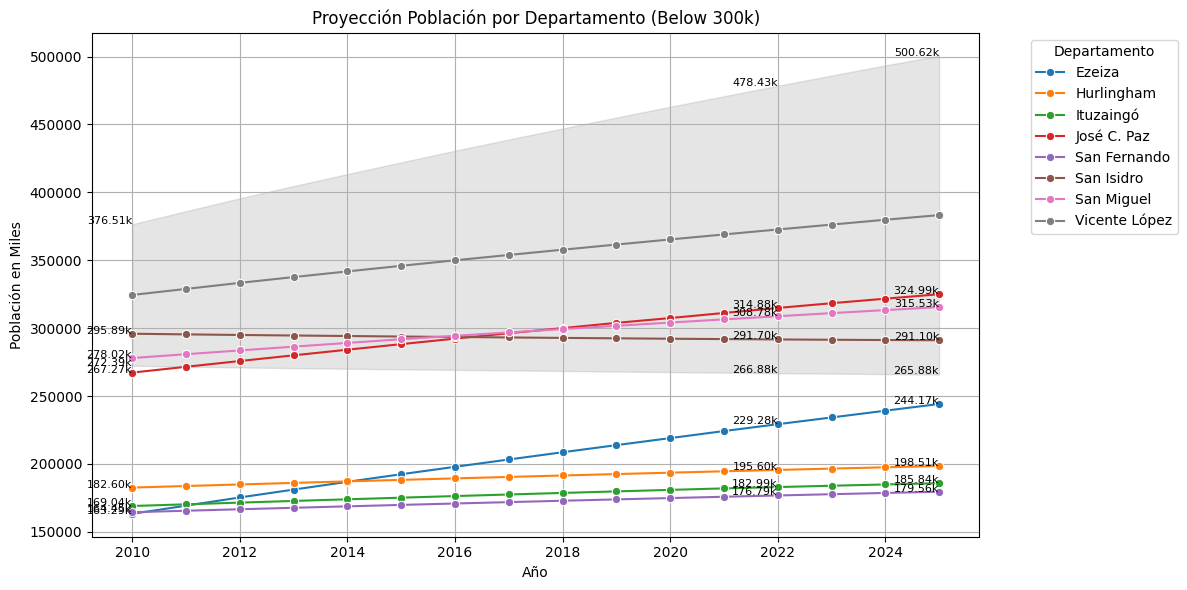
\includegraphics[width=0.8\textwidth]{{C:/Users/Fer/ITBA_TFI/code/latex/img/ProyLineas300k.png}}
  \caption{Población por departamento 2010-2025.INDEC}
  \label{fig:proy300k}
\end{figure}

\begin{figure}[htbp]
  \centering
  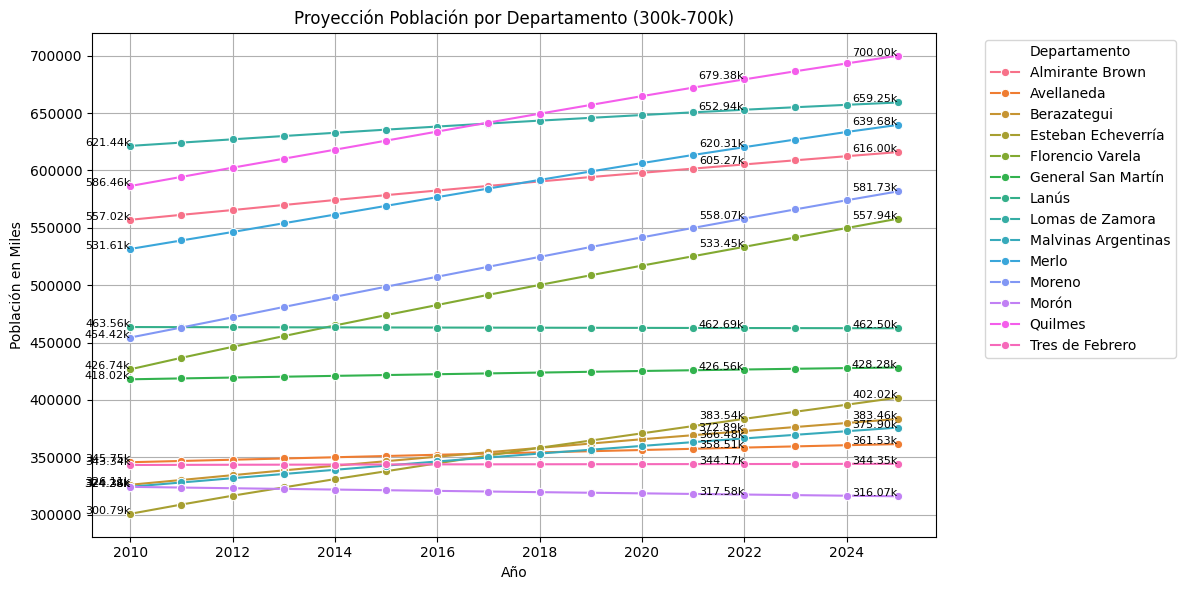
\includegraphics[width=0.8\textwidth]{{C:/Users/Fer/ITBA_TFI/code/latex/img/ProyLineas700k.png}}
  \caption{Población por departamento 2010-2025.INDEC}
  \label{fig:proy700k}
\end{figure}
\begin{figure}[htbp]
  \centering
  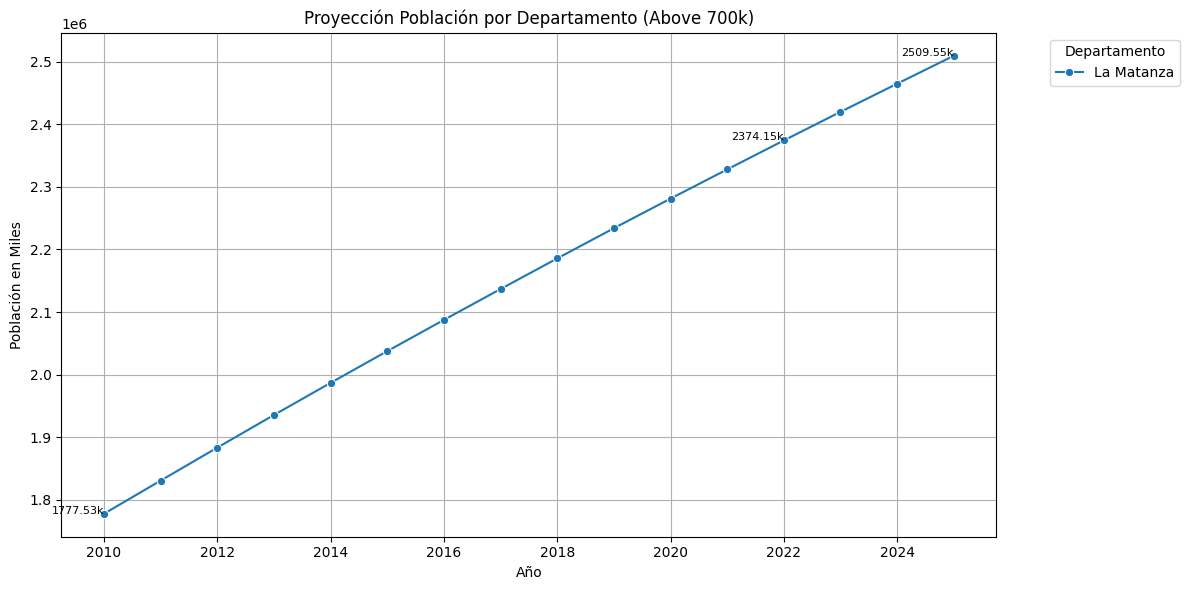
\includegraphics[width=0.8\textwidth]{{C:/Users/Fer/ITBA_TFI/code/latex/img/ProyLineas1.300k.png}}
  \caption{Población por departamento 2010-2025.INDEC}
  \label{fig:proyMayor700k}
\end{figure}

\subsection{Componente geográfico }
Con el objetivo de enriquecer el dataset se incorpora una tabla con los polígonos geográficos de cada departamento.
 La misma se obtiene del Instituto Geográfico Nacional (IGM) [10], de donde se obtiene la capa SIG para 
 todos los departamentos de la República Argentina. Luego se cruza con el listado de departamentos del AMBA , generando un dataset con las caracteristicas geográficas 
 sumadas a  los datos censales recopilados desde 1991 a 2022.

\begin{table}[htbp]
    \centering
    \caption{Descripción de Variables Geográficas}
    \begin{tabular}{|l|l|p{8cm}|}
        \hline
        \textbf{Variable} & \textbf{Nombre} & \textbf{Descripción} \\
        \hline
        geom & geometry & Polígono WKT con los límites del departamento \\
        fna & Nombre geográfico & Nombre completo que se utiliza para designar un objeto en un mapa o carta. Está formado por el término genérico y el término específico. Ejemplo: río Mendoza. \\
        gna & Término genérico & Parte del nombre geográfico que indica el tipo de objeto que identifica. Ejemplo: río, monte, glaciar, establecimiento. \\
        nam & Término específico & Parte de un nombre geográfico que acompaña al término genérico y que identifica e individualiza un objeto geográfico determinado. Ejemplo: Paraná en río Paraná; Upsala en glaciar Upsala; Las Marías en establecimiento Las Marías; Esperanza en el caso de bahía Esperanza. \\
        in1 & Código INDEC & Código único de vías de circulación asignado por el Instituto Nacional de Estadística y Censos de la República Argentina. \\
        fdc & Fuente de captura & Identificación del nombre y tipo de fuente utilizada para capturar la información. Puede incluir fecha y otros datos adicionales. \\
        sag & Autoridad de fuente & Nombre de la autoridad responsable de la información utilizada. \\
        \hline
    \end{tabular}
    \label{tab:geo.depto}
\end{table}



%%%%%%%%%%%%%%%%%%%%%%%%%%%%%%%%

\subsection{Población}

Con sustento en la base de datos "AMBA" ( POSTGRES/POSTGIS) se analizarán los distintos datos recopilados según nivel de agregación.
En primera instancia se  generó un dataset con todos los departamentos del AMBA, sus caracteristicas georgráficas así como los valores
de las variables correspondientes a los censos 1991-2001-2010-2022.\ref{fig:lineasPob}
 
En el cuadro \ref{tab:censos_amba} se puede observar el esquema del dataset .
\begin{table}[htb]
  \centering
  \footnotesize
  \begin{tabular}{|c|c|c|c|c|c|c|c|c|c|c|}
  \hline
    \textbf{\cellcolor[rgb]{0,0.231,0.427}\textcolor{white}{nam}} &
   \textbf{\cellcolor[rgb]{0,0.231,0.427}\textcolor{white}{$cod_depto$}} 
   & \textbf{\cellcolor[rgb]{0,0.231,0.427}\textcolor{white}{anio}} &
   \textbf{\cellcolor[rgb]{0,0.231,0.427}\textcolor{white}{pob}} & 
   \textbf{\cellcolor[rgb]{0,0.231,0.427}\textcolor{white}{var}} & 
   \textbf{\cellcolor[rgb]{0,0.231,0.427}\textcolor{white}{muj}} &
    \textbf{\cellcolor[rgb]{0,0.231,0.427}\textcolor{white}{vivpart}} & 
    \textbf{\cellcolor[rgb]{0,0.231,0.427}\textcolor{white}{vivtotal}} &
     \textbf{\cellcolor[rgb]{0,0.231,0.427}\textcolor{white}{sup}} &
      \textbf{\cellcolor[rgb]{0,0.231,0.427}\textcolor{white}{$ind_masc$}} &
       \textbf{\cellcolor[rgb]{0,0.231,0.427}\textcolor{white}{$dens_pob$}} \\
  \hline
  Almirante Brown & 06028 & 1991 & 450698.0 & 222042.0 & 228656.0 & nan & nan & 157.87 & 97.1 & 2854.87 \\
  Almirante Brown & 06028 & 2010 & 552902.0 & 270247.0 & 282655.0 & 156218.0 & 78.0 & 157.87 & 95.6 & 3502.26 \\
  Almirante Brown & 06028 & 2022 & 585852.0 & 281842.0 & 301779.0 & 184403.0 & 60.0 & 157.87 & 93.4 & 3710.98 \\
  Almirante Brown & 06028 & 2001 & 515556.0 & 252454.0 & 263102.0 & 143543.0 & 88.0 & 157.87 & 96.0 & 3265.70 \\
  Avellaneda & 06035 & 2001 & 328980.0 & 155450.0 & 173530.0 & 117200.0 & 59.0 & 68.54 & 89.6 & 4799.82 \\
  Avellaneda & 06035 & 1991 & 344991.0 & 164243.0 & 180748.0 & nan & nan & 68.54 & 90.9 & 5033.43 \\
  Avellaneda & 06035 & 2010 & 342677.0 & 162264.0 & 180413.0 & 121307.0 & 68.0 & 68.54 & 89.9 & 4999.66 \\
  Avellaneda & 06035 & 2022 & 370939.0 & 174572.0 & 194911.0 & 144988.0 & 64.0 & 68.54 & 89.6 & 5412.01 \\
  Berazategui & 06091 & 2010 & 324244.0 & 158608.0 & 165636.0 & 96029.0 & 37.0 & 268.91 & 95.8 & 1205.77 \\
  Berazategui & 06091 & 2022 & 360582.0 & 173892.0 & 186255.0 & 117699.0 & 37.0 & 268.91 & 93.4 & 1340.90 \\
  ...... &  &  &  &  &  & &  &  &  &  \\ \hline
  \end{tabular}
  \caption{Dataset Censos AMBA}
  \label{tab:censos_amba}
  \end{table}
  
  Se observa en el cuadro \ref{tab:summaryCensos} que existen valores nulos para el valor poblaciones, que se corresponden,
   con los casos de municipios de desaparecen en la reorganización administrativa desde 1991 a 2001.\newline
    A saber : Esteban Echeverría' ,'Ezeiza', 'Florencio Varela' ,'Hurlingham' 'Ituzaingó'
    'José C. Paz', 'Malvinas Argentinas', 'Morón' ,'San Miguel' y     'General Sarmiento'.
   \newline Se destaca también que    para el censo 1991 no se detalla el total de viviendas particules y colectivas .

\begin{table}[htbp]
    \centering
    \caption{Summary de columnas de Censos AMBA}
    \label{tab:summaryCensos}
    \begin{tabular}{llll}
        \toprule
        \textbf{Column} & \textbf{Non-Null Count} & \textbf{Dtype} \\
        \midrule
        nam & 96 & object \\
        cod\_depto & 96 & object \\
        anio & 96 & object \\
        pob & 90 & float64 \\
        var & 90 & float64 \\
        muj & 90 & float64 \\
        vivpart & 72 & float64 \\
        vivtotal & 72 & float64 \\
        sup & 96 & object \\
        ind\_masc & 90 & object \\
        dens\_pob & 90 & object \\
        \bottomrule
    \end{tabular}
\end{table}


\begin{figure}[htbp]
  \centering
  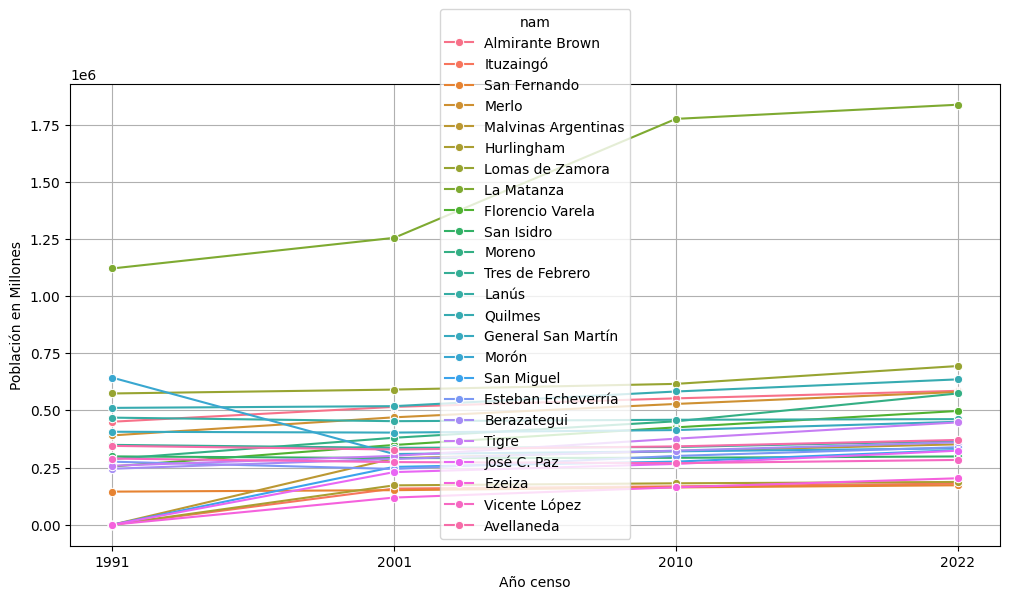
\includegraphics[width=0.8\textwidth]{{C:/Users/Fer/ITBA_TFI/code/latex/img/Pob19912022All.png}}
  \caption{Población por departamento 1991-2022}
  \label{fig:lineasPob}
\end{figure}

Asismismo se analiza la evolución de la densisdad de población [hab/\textup{km\textsuperscript{2}}], la misma puede obsersevarse
en la figura \ref{fig:lineasDensAll}. Las mismas consideraciones aplican en el caso de densidad respecto a los departamentos que sufren
modificaciones administrativas entre 1991  y 2001, donde los valores de densidad se ven fuertemente afectados y no pueden asociarse
al fenómeno poblacional.

\begin{figure}[htbp]
  \centering
  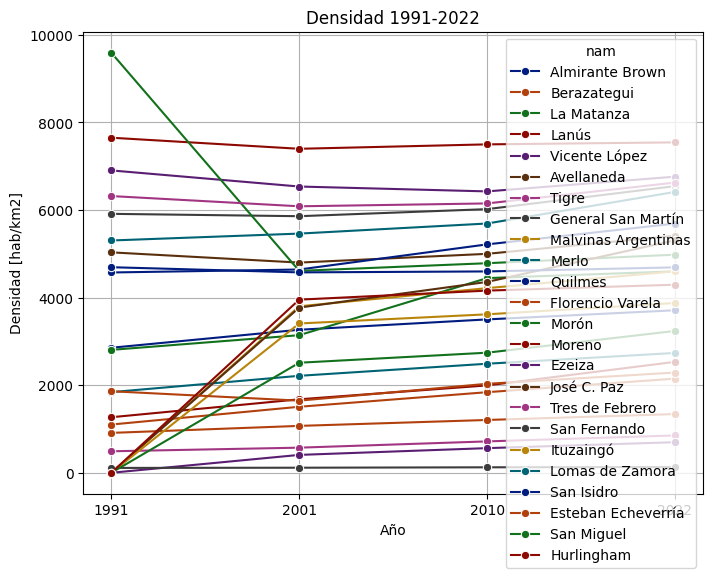
\includegraphics[width=0.8\textwidth]{{C:/Users/Fer/ITBA_TFI/code/latex/img/Dens199122All.png}}
  \caption{Densidad de Población por departamento 1991-2022}
  \label{fig:lineasDensAll}
\end{figure}


\subsubsection{Población.Vista geográfica}

En este caso se busca una visualización geográfica del dataset. Utilizando el sofware QGIS conectado directamente a la base de 
datos AMBA (POSTGRES) se pudo disponer la información de cada Departamento con su geolocalización.
 Se detalla en la figura \ref{fig:AllPob} la poblacion total para cada departamento (Censos 1991 -2022).Se observa claramente que el distrito más poblado 
 es La Matanza.

%%% QGIS GRAPHICS
\begin{landscape}
\begin{figure}[p] % Use 'p' to force the figures to be placed on a separate page
  \centering
  \begin{subfigure}[b]{0.48\textwidth}
      \centering
      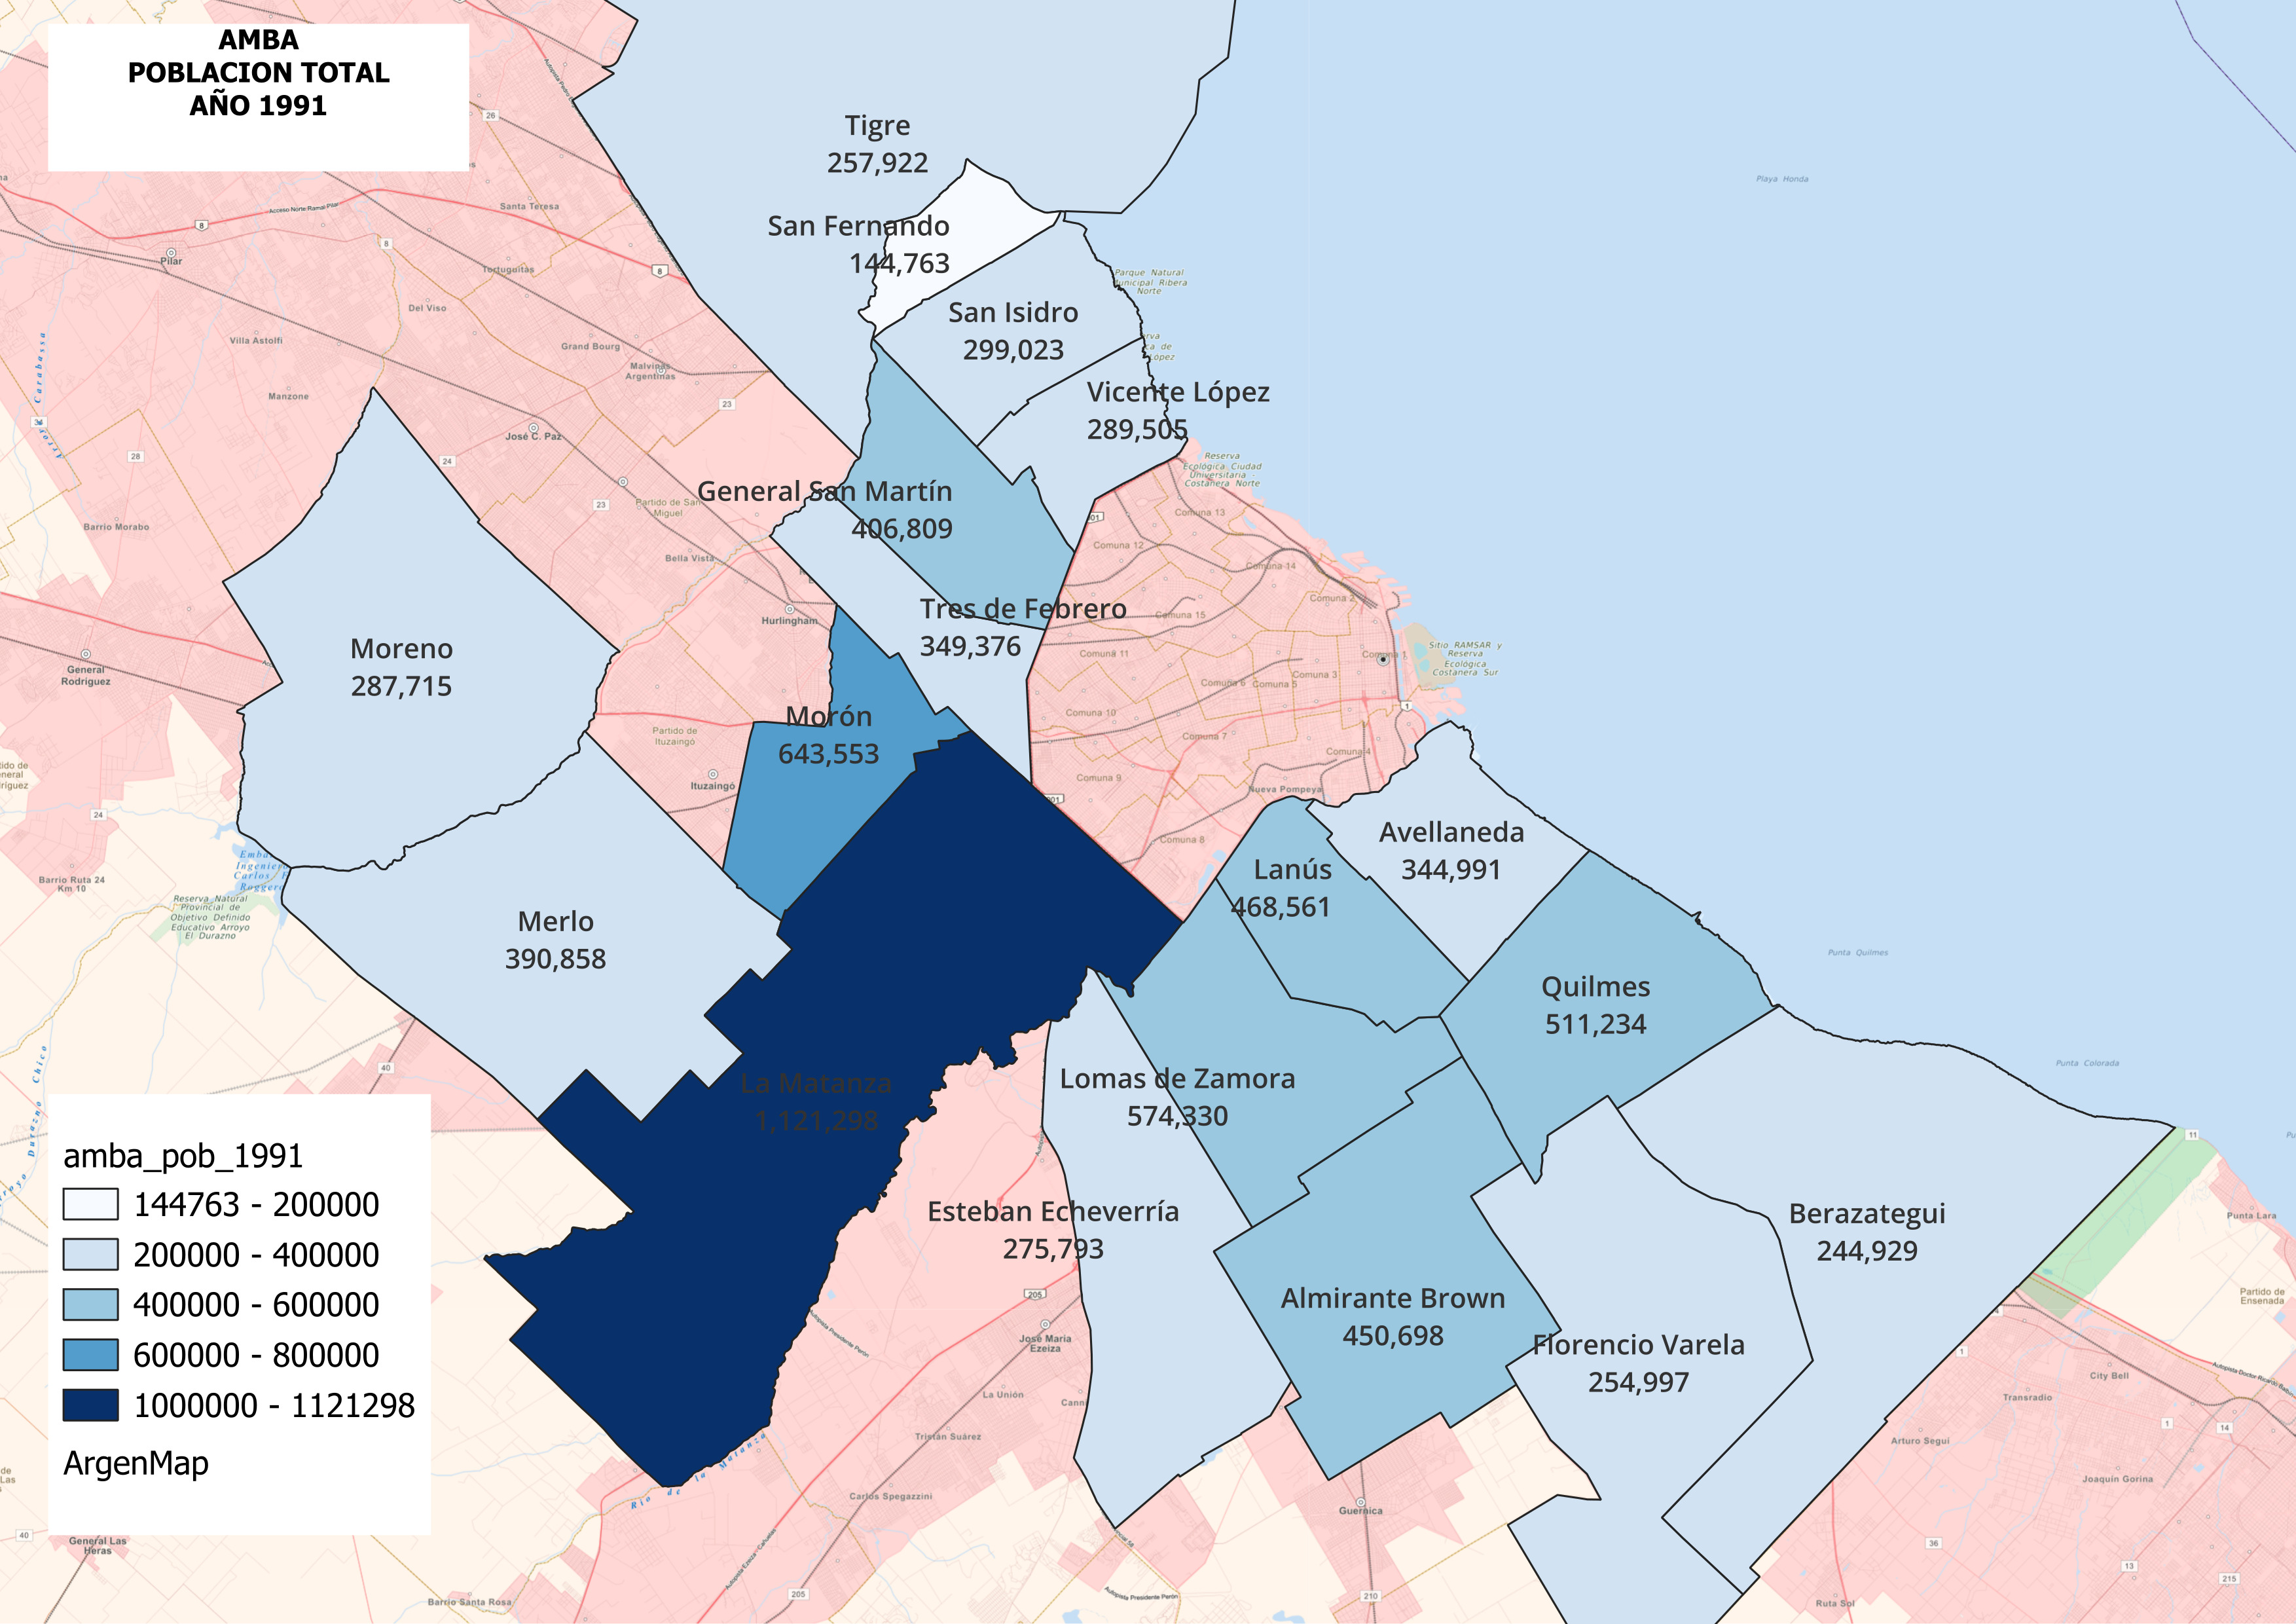
\includegraphics[width=\textwidth]{{C:/Users/Fer/ITBA_TFI/QGIS/img/AmbaPob1991.jpg}}
      \caption{AMBA- Población total Censo 1991}
      \label{fig:pob1991}
  \end{subfigure}
  \quad % Add some horizontal space between subfigures
  \begin{subfigure}[b]{0.48\textwidth}
      \centering
      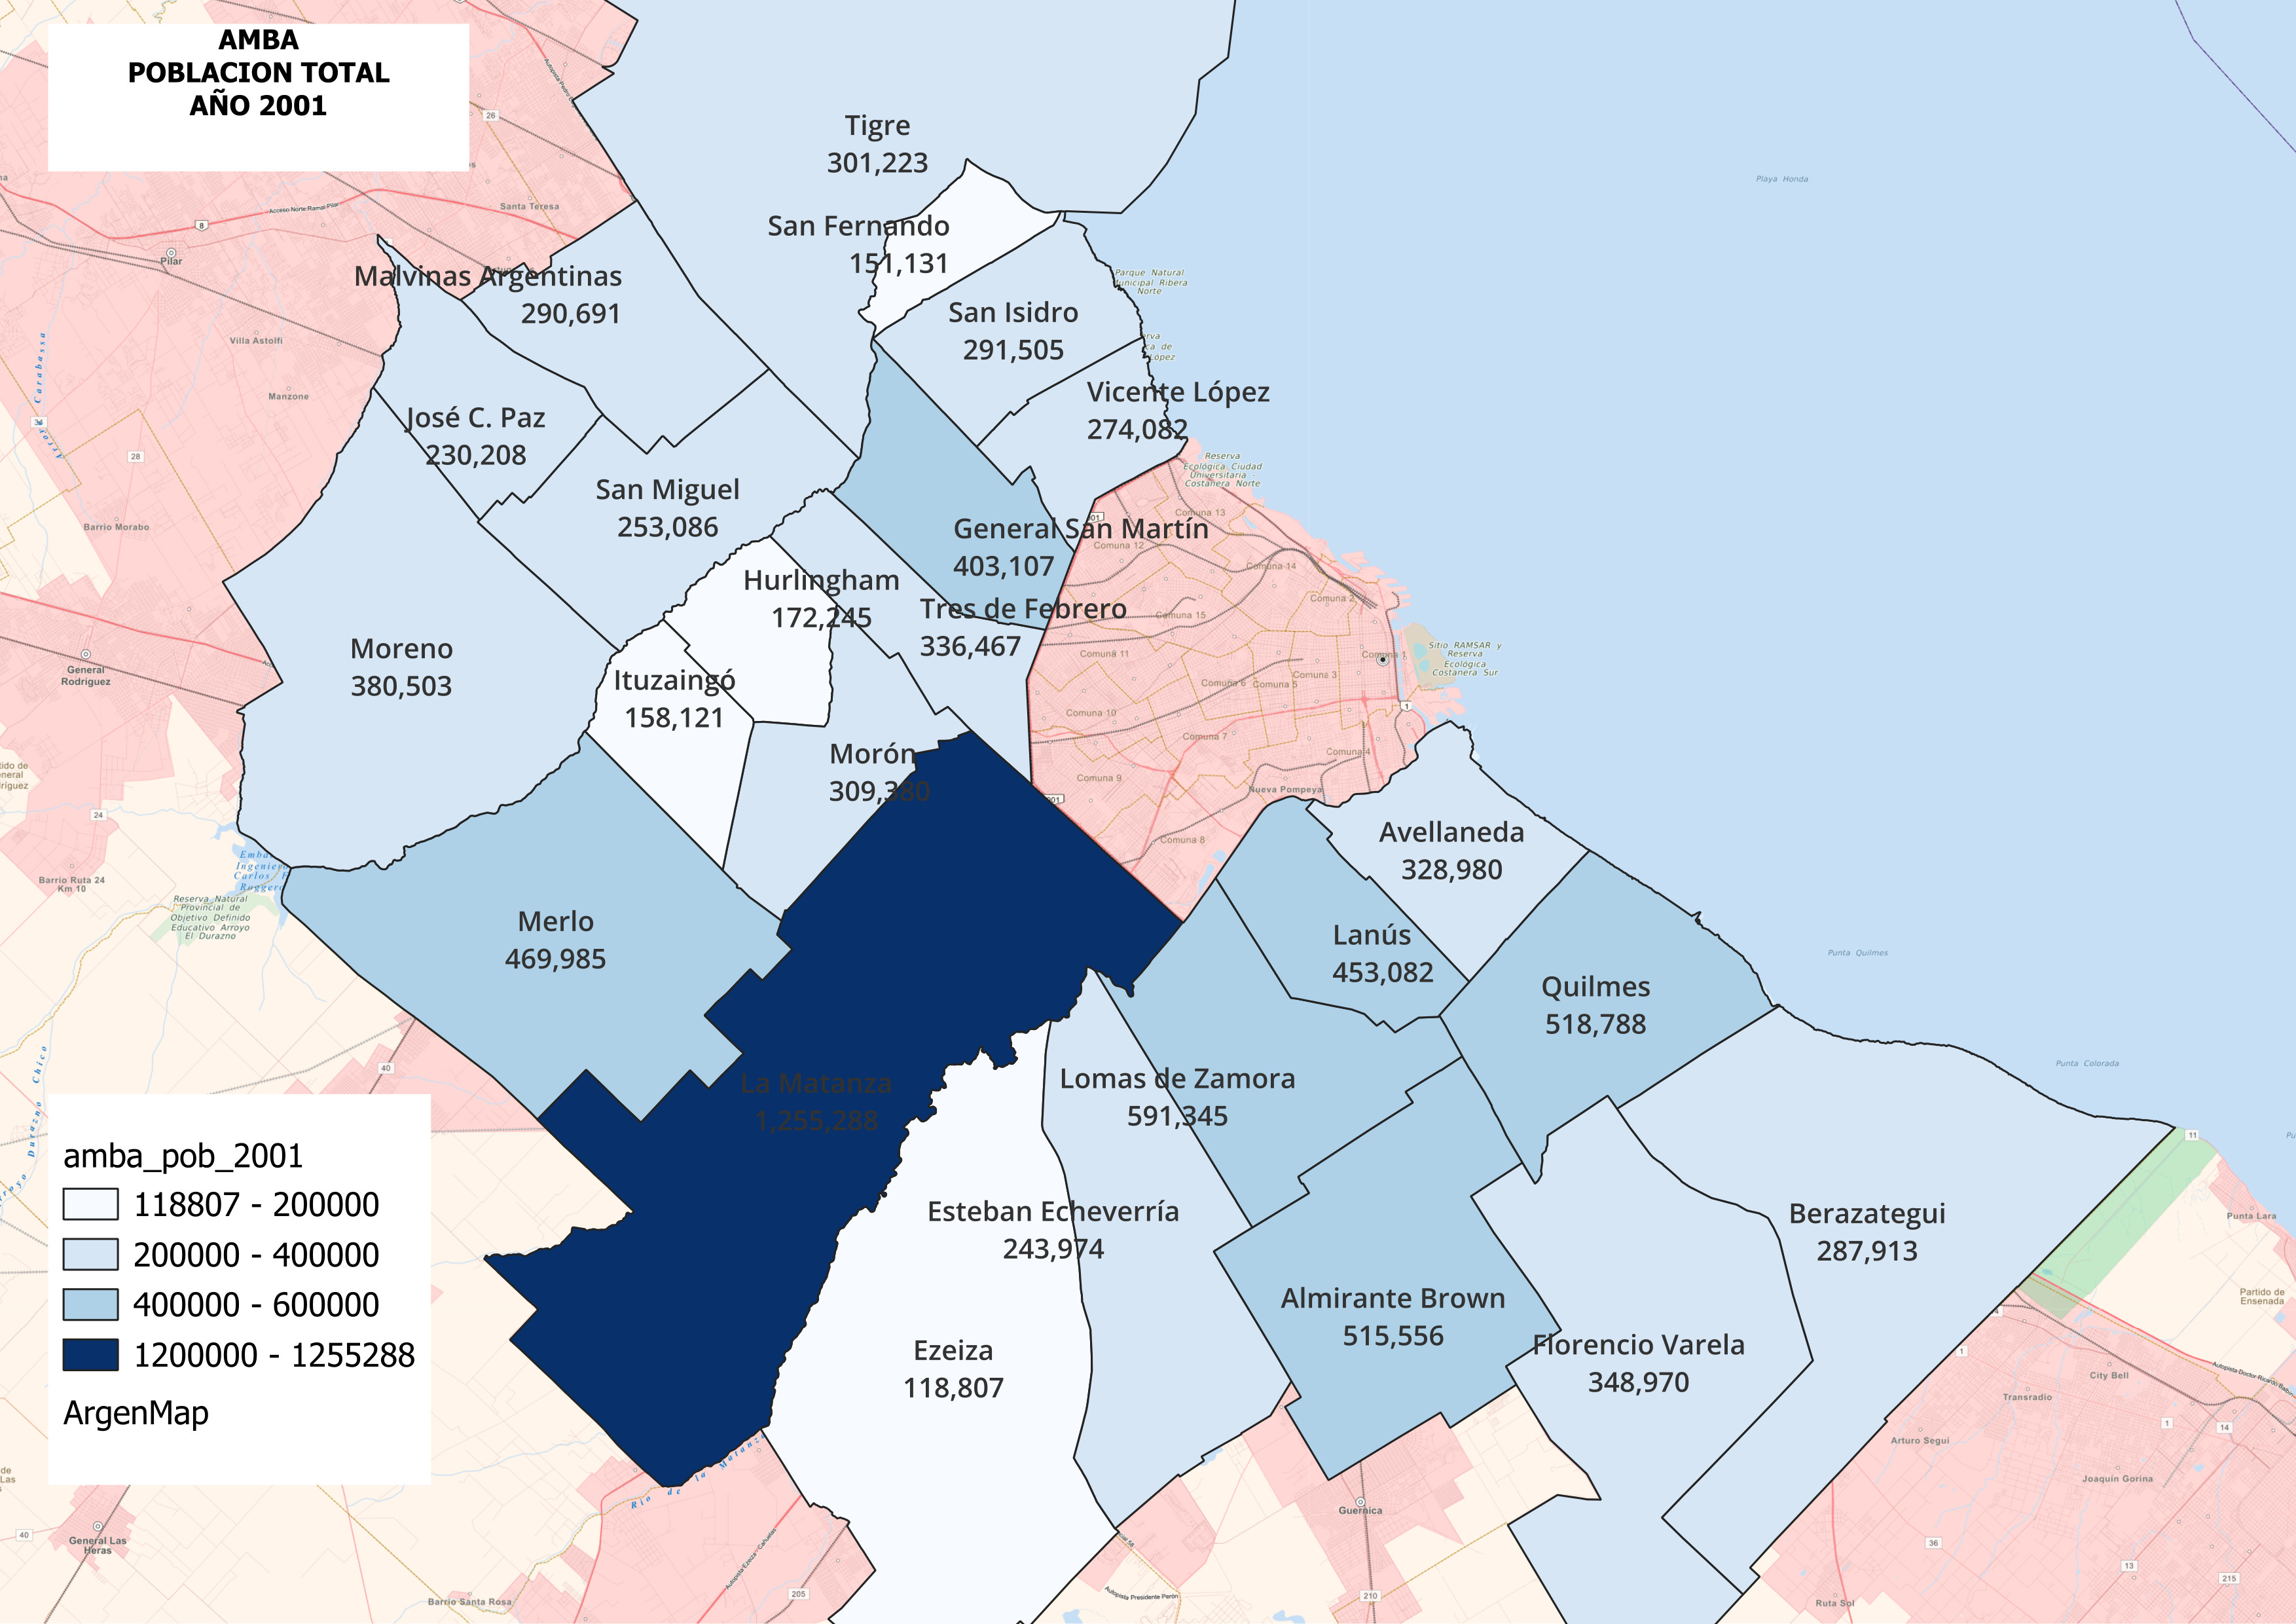
\includegraphics[width=\textwidth]{{C:/Users/Fer/ITBA_TFI/QGIS/img/AmbaPob2001.jpg}}
      \caption{AMBA- Población total Censo  2001}
      \label{fig:pob2001}
  \end{subfigure}
  
  \begin{subfigure}[b]{0.48\textwidth}
      \centering
      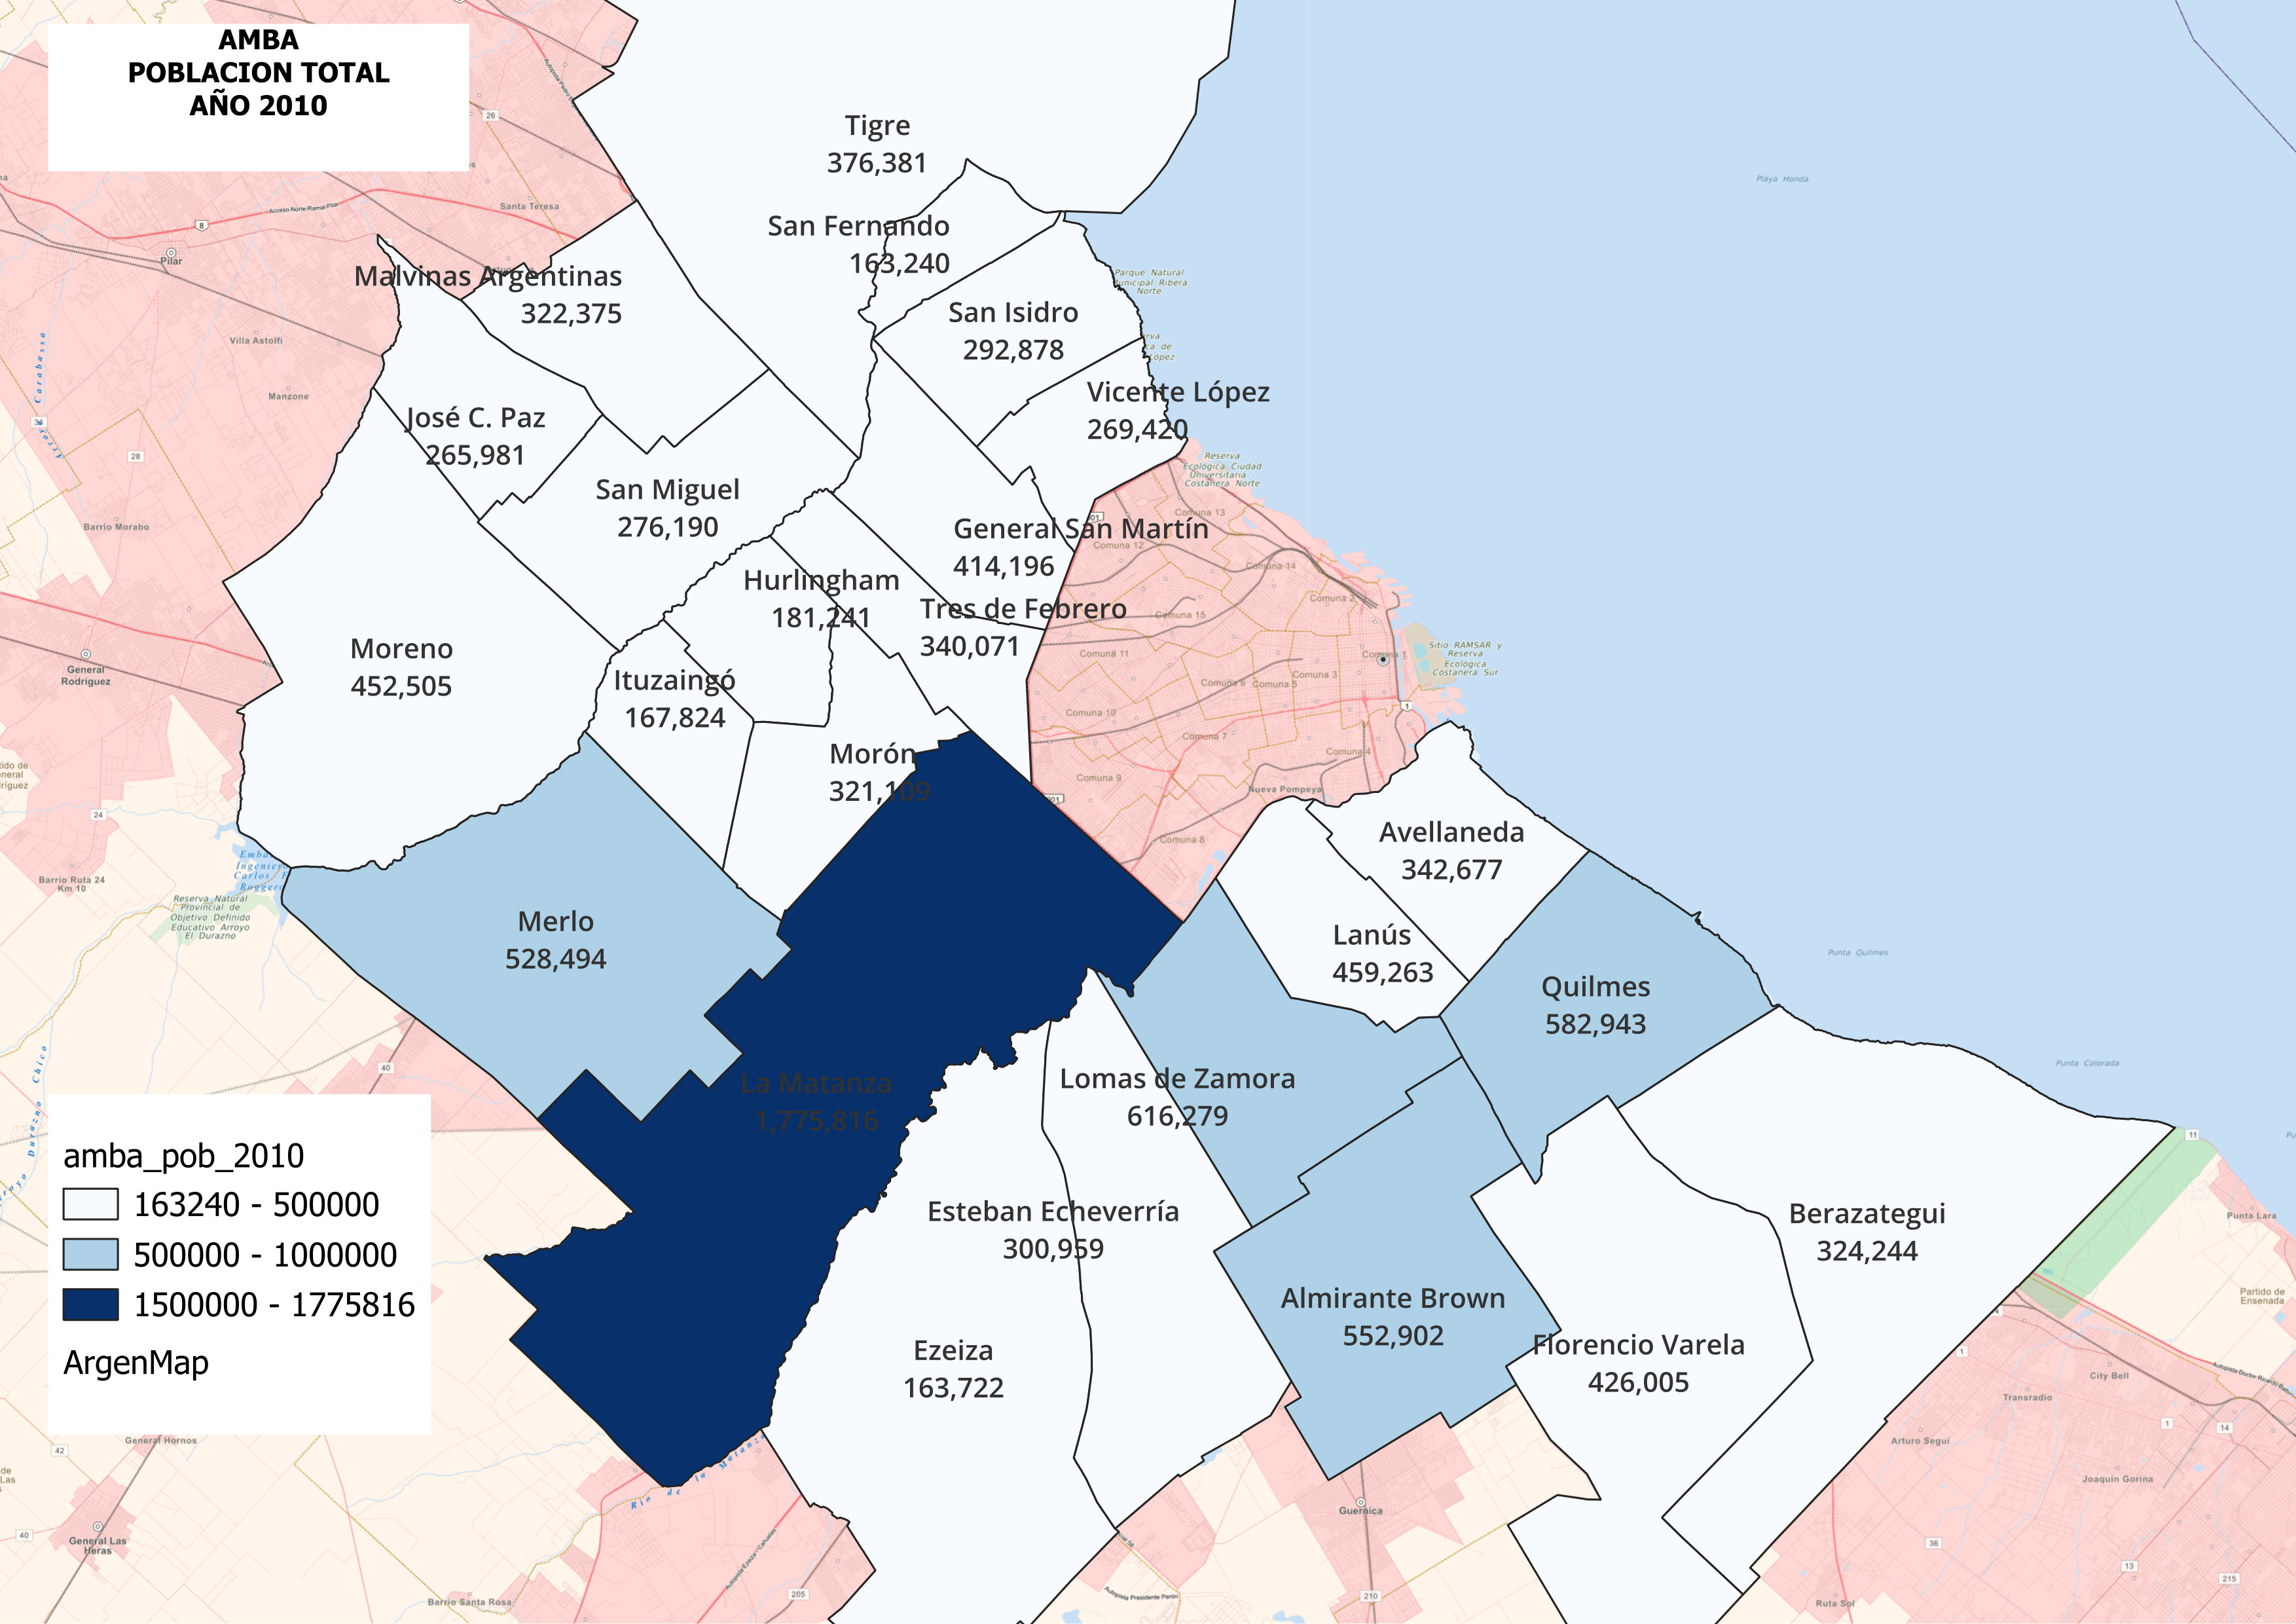
\includegraphics[width=\textwidth]{{C:/Users/Fer/ITBA_TFI/QGIS/img/AmbaPob2010.jpg}}
      \caption{AMBA- Población total Censo 2010}
      \label{fig:pob2010}
  \end{subfigure}
  \quad % Add some horizontal space between subfigures
  \begin{subfigure}[b]{0.48\textwidth}
      \centering
      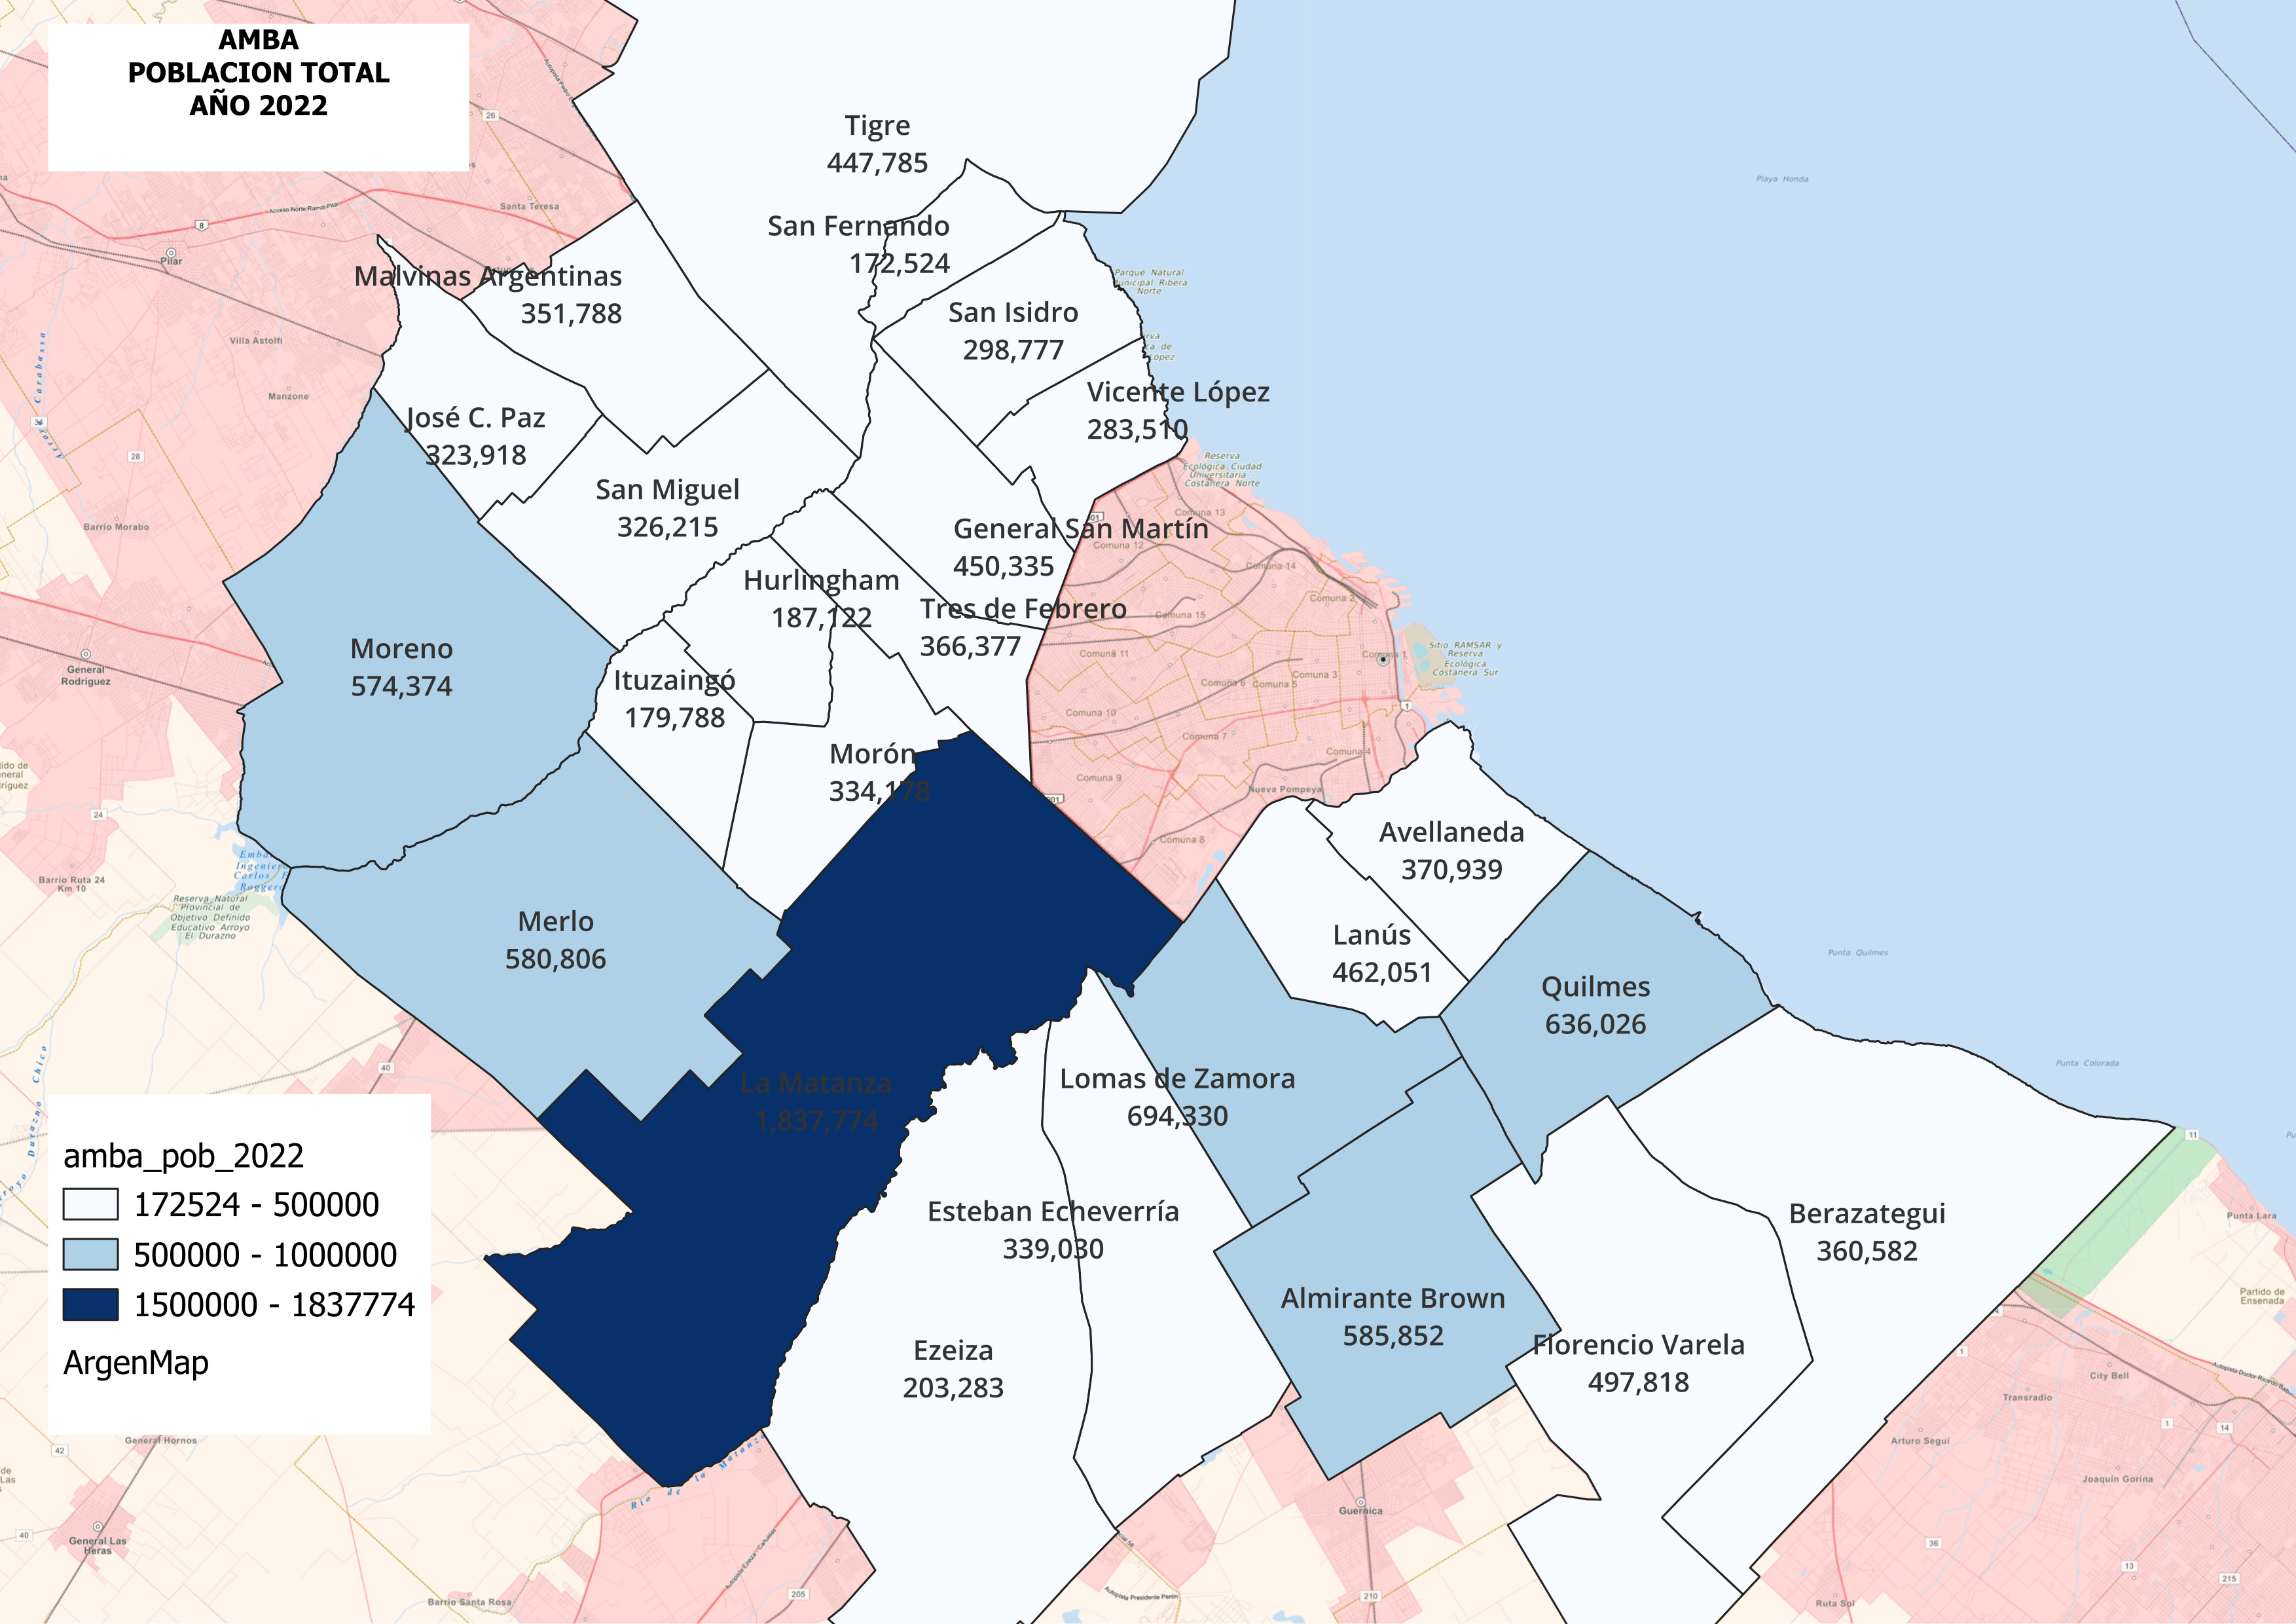
\includegraphics[width=\textwidth]{{C:/Users/Fer/ITBA_TFI/QGIS/img/AmbaPob2022.jpg}}
      \caption{AMBA- Población total Censo 2022}
  \label{fig:pob2022}
  \end{subfigure}
  \caption{Población Total Censos 1991 2022}
\label{fig:AllPob}
\end{figure}
\end{landscape}


 \subsubsection{Población - Ratios de crecimento}
  En este caso se determinaron los ratios de crecimento entre censos consecutivos para cada departamento.
  Para este análisis se trata de manera difrenciada aquellos municipios que han sufrido modificaciones administrativas
  desde 1991  a 2001, donde se  que al  desmembrarse en varios partidos, resignando superficie, algunas tasas o ratios de crecimiento 
  se muestran negativos. Asimismo partidos que ha visto incrementada su superfice presentan  tasas de crecimiento no representativas del 
  fenómeno demográfico.\newline
  Por otra parte partidos que desaparecen o se crean en el año  2001 no se consideran el valor del ratio para el intervalo 1991-2001.\newline
    En el cuadro \ref{tab:RatiosAll} se puede observar los valores obtenidos. Para el año en cuestion la tasa surge de dividir el valor poblacional
  del censo de este año sobre el valor poblacional del censo anterior,expresado en porcentaje.\newline
  Es decir: \newline
  \begin{equation}
    \underset{\text{\footnotesize(Año $X$)}}{\text{Growth Ratio}} = 
    \left( \frac{\underset{\text{\footnotesize(Censo $X$)}}{\text{Población}}}{\underset{\text{\footnotesize(Censo $X-1$)}}{\text{Población}}} - 1 \right) \times 100
  \end{equation}
  \newline

  \begin{table}[htb]
    \centering
    \begin{tabular}{|c|c|c|c|}
    \hline
    \textbf{\cellcolor[rgb]{0,0.231,0.427}\textcolor{white}{nam}} &
     \textbf{\cellcolor[rgb]{0,0.231,0.427}\textcolor{white}{anio}}
      & \textbf{\cellcolor[rgb]{0,0.231,0.427}\textcolor{white}{pob}}
       & \textbf{\cellcolor[rgb]{0,0.231,0.427}\textcolor{white}{$growth_ratio$}} \\ \hline
    Almirante Brown & 2001 & 515556.0 & 14.39 \\
    Almirante Brown & 2022 & 585852.0 & 5.96 \\
    Almirante Brown & 2010 & 552902.0 & 7.24 \\
    Avellaneda & 2001 & 328980.0 & -4.64 \\
    Avellaneda & 2010 & 342677.0 & 4.16 \\
    Avellaneda & 2022 & 370939.0 & 8.25 \\
    Berazategui & 2022 & 360582.0 & 11.21 \\
    Berazategui & 2001 & 287913.0 & 17.55 \\
    Berazategui & 2010 & 324244.0 & 12.62 \\
    Esteban Echeverría & 2001 & 243974.0 & -11.54 \\
    Esteban Echeverría & 2010 & 300959.0 & 23.36 \\
    Esteban Echeverría & 2022 & 339030.0 & 12.65 \\
    Ezeiza & 2022 & 203283.0 & 24.16 \\
    Ezeiza & 2010 & 163722.0 & 37.81 \\
    ....& & & \\
  
    \hline
    \end{tabular}
    \caption{Extracto. Tasa de crecimiento Intercensal}
  \label{tab:RatiosAll}
    \end{table}
  

  A partir de  análisis estadísitico simple sobre estas tasas se observa una gran disparidad en los valores, siendo que se trata de un sector
  geográfico de similares características demográficas. Cuadro \ref{tab:summary_growth_ratio}
\begin{table}[htbp]
    \centering
    \begin{tabular}{lr}
        \hline
        \textbf{Estadístico} & \textbf{Valor} \\
        \hline
        Count & 66.000000 \\
        Mean & 9.286961 \\
        Standard Deviation & 13.111467 \\
        Minimum & -51.926259 \\
        25\% Percentile & 3.033150 \\
        50\% Percentile & 8.129835 \\
        75\% Percentile & 16.476163 \\
        Maximum & 41.466819 \\
        \hline
    \end{tabular}
    \caption{Summary Statistics for Growth Ratio}
    \label{tab:summary_growth_ratio}
\end{table}
\newline
A partir de la elaboración de un gráfico boxplot se determinaron los \textbf{Outliers} para estas tasas de crecimiento.

\begin{figure}[htbp]
  \centering
  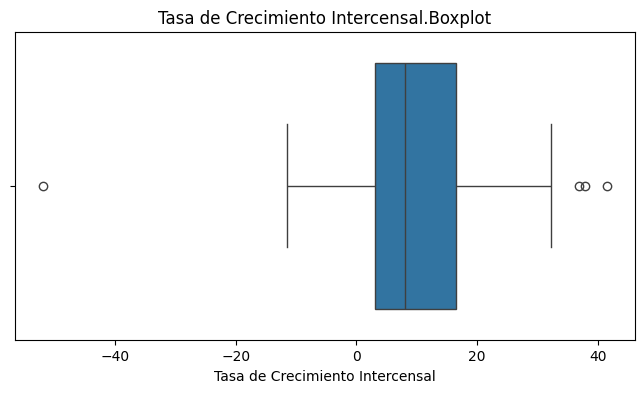
\includegraphics[width=0.8\textwidth]{{C:/Users/Fer/ITBA_TFI/code/latex/img/GrowthRatioBoxplot.png}}
  \caption{Box plot Tasas de crecmiento intercensa 1991-2022}
  \label{fig:boxplotRatios}
\end{figure}
 En este caso en el cuadro \ref{fig:boxplotRatios} se observan 4 outliers , tanto en valores positivos como negativos. Como se comentó anteriormente no se analizarán
 los casos con modificaciones admitrativas desde 1991 a 2001.Cuadro \ref{tab:DimDepto} .Se desestima el caso de Morón para el período 1991-2001 donde la tasa 
 es negativa de 51.9, debido a la cesión de tierras para la creación de distintos partidos.\newline

\begin{table}[htbp]
  \centering
  \begin{tabular}{|c|c|c|c|r|r|}
      \hline
      \textbf{id} & \textbf{nam} & \textbf{codDepto} & \textbf{anio} & \textbf{pob} & \textbf{growthRatio} \\
      \hline
      54 & Morón & 06568 & 2001 & 309380.0 & -51.92 \\
      78 & Florencio Varela & 06274 & 2001 & 348970.0 & 36.85 \\
      13 & La Matanza & 06427 & 2010 & 1775816.0 & 41.47\\
      29 & Ezeiza & 06270 & 2010 & 163722.0 & 37.80 \\
      \hline
  \end{tabular}
  \caption{Outliers para Tasas de crecmiento intercensal}
\label{tab:RatiosOutliers}
\end{table}

Se  grafica a continación (Figura \ref{fig:OutlierlineasPob}) la curva población de los 3 outiliers destacados :Florencio Varela ,La Matanza y Ezeiza.


\begin{figure}[htbp]
  \centering
  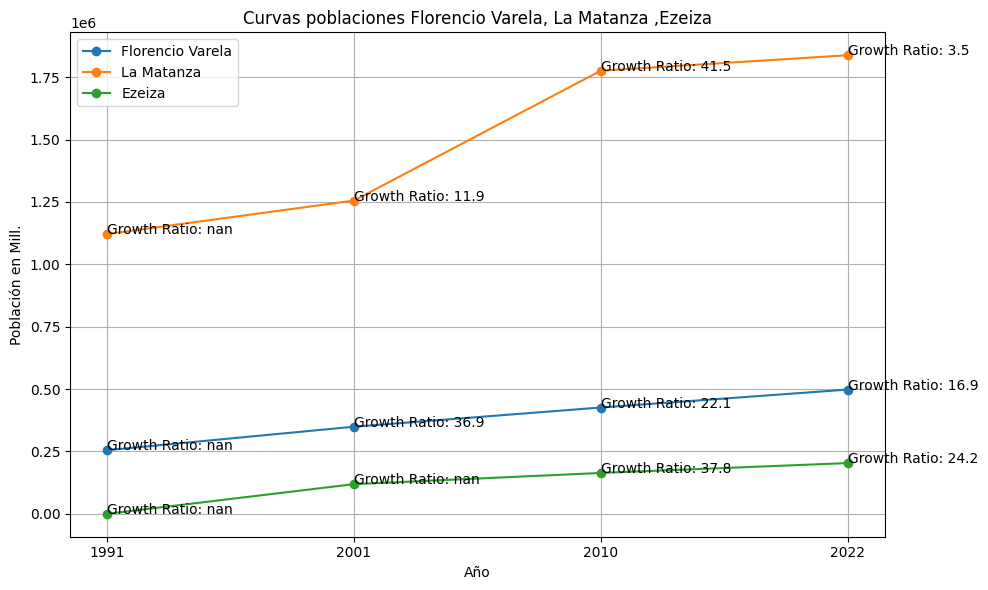
\includegraphics[width=0.8\textwidth]{{C:/Users/Fer/ITBA_TFI/code/latex/img/CurvasOutliersRatios.png}}
  \caption{Curvas de Población por departamento 1991-2022}
    \label{fig:OutlierlineasPob}
\end{figure}


\subsubsection{ Tasas de crecimento intercensal.Coeficiente de Variación}
 Con el objetivo de profundizar el análsis de las tasas de crecimiento
 se procedió a calcular luego la desviación estandar y el coeficiente de variación por Departamento.\newline
En primera instancia se agrupa por departamento para determinar la media y la desviación estándar de cada subset de datos.
Se define  el coeficiente de variación (CV) como:

\begin{equation}
  \underset{\text{\footnotesize(Departametno)}}{\text{CV}} = 
  \left( \frac{\underset{\text{\footnotesize(Departamento)}}{\text{Std.Dev}}}{\underset{\text{\footnotesize(Departamento)}}{\text{Mean}}} \right) \times 100
\end{equation}

El coeficiente de variación es una medidad de la dispersión alrededor de la media de la población. En este caso sería curvas poblacionales
con gran dispersión en su tasas de crecimento para los censos del periodo analizado año 1991 -2022.-
\newline
En la figura \ref{fig:CVOutliersPoblacion} se observa el resultado .Se destaca en particular los valores extremos
tanto negativos como positivos.A saber : Vincente López, Morón, Tres de Febrero, Avellaneda ,La Matanza ,
Esteban Echeverría, General San Martín.  
\newline 
Cabe recordar en este instancia que los partidos de Esteban Echeverría,
 Florencio Varela y Morón sufrieron modificaciones administrativa en el período 1991-2001.
 En la figura \ref{fig:CVoutCurvasMedia} así como en la figura\ref{fig:CVoutCurvasAlta} puede observarse la curvas poblacionales
 de los departamentos destacados.\newline
En estos casos se prestará particular atención a las predicciones hechas por el INDEC así como las metodologías que se implementen 
para la estimación de la curva poblacional, es esperable una mayor error de prediccion en estos casos cuyas curvas prensetan singularidades respecto a
los municipios inmediatamente aledaños.


\begin{figure}[htbp]
  \centering
  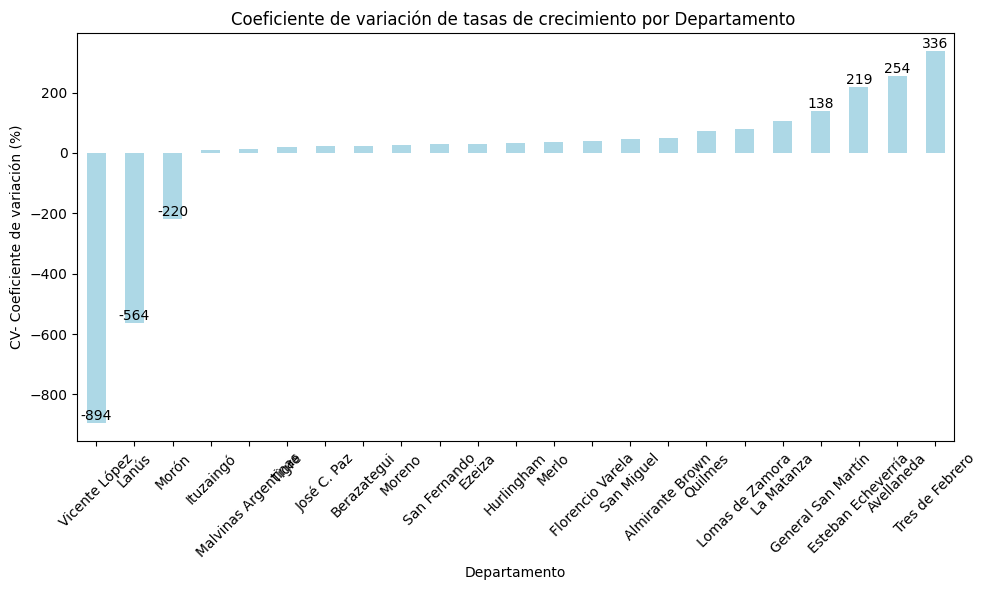
\includegraphics[width=0.8\textwidth]{{C:/Users/Fer/ITBA_TFI/code/latex/img/CVGrowthRatioAll.png}}
  \caption{CV.Coeficiente de variación por departamento -1991-2022}
\label{fig:CVOutliersPoblacion}
\end{figure}

 
\begin{figure}[htbp]
  \centering
  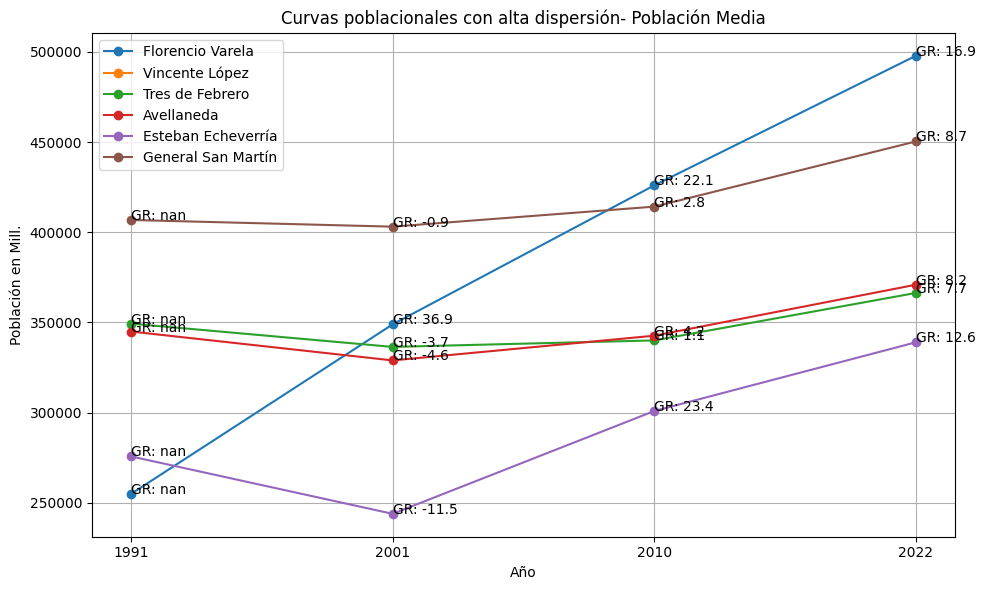
\includegraphics[width=0.45\textwidth]{{C:/Users/Fer/ITBA_TFI/code/latex/img/CurvasCVOutliersPobMedia.png}}
  \caption{Curvas poblacionales de alta dispersión - Población Media}
  \label{fig:CVoutCurvasMedia}
\end{figure}

\begin{figure}[htbp]
  \centering
  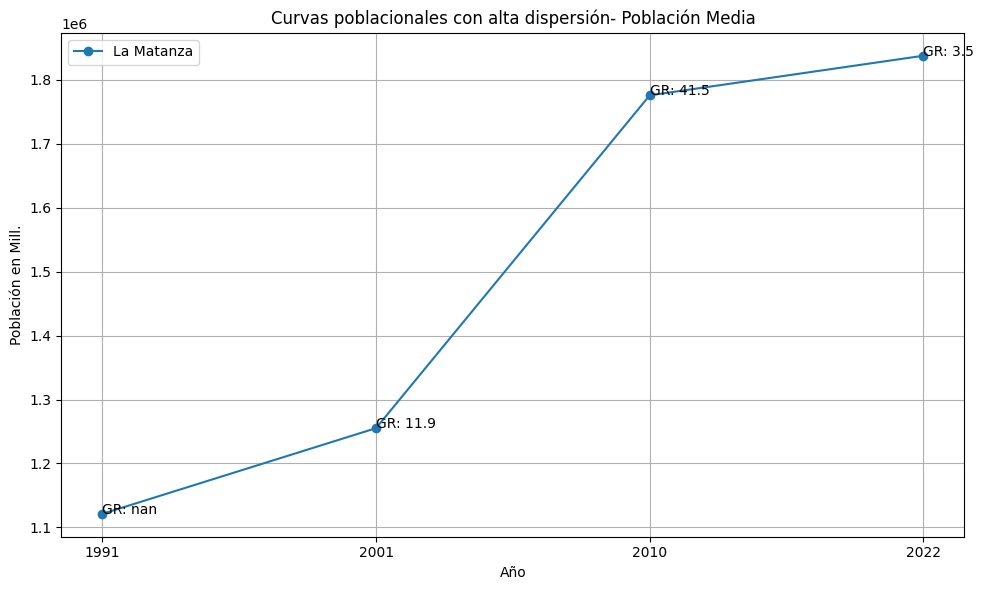
\includegraphics[width=0.45\textwidth]{{C:/Users/Fer/ITBA_TFI/code/latex/img/CurvasCVOutliersPobAlta.png}}
  \caption{Curvas poblacionales de alta dispersión - Población Alta}
\label{fig:CVoutCurvasAlta}
\end{figure}


\subsection{Densidad de Población}

En el dataset se incorpora la densidad de población en habitantes/\textup{km\textsuperscript{2}}, lógicamente estos valores 
se ven notablemente afectados por la reorganización político administrativa desde 1991 a 2001.\newline
Si analizamos la distribución de los valores de densidad para cada censo, puede observarse distribuciones homogeneas simétricas, 
con un incremento en al mediana de cada población censal desde 2001 a 2022.  El análisis univariado de esta variable puede observarse 
en la figura\ref{fig:DensPoblBoxplot}  y la figura\ref{fig:DensPoblLineas}.

\begin{figure}[htbp]
  \centering
  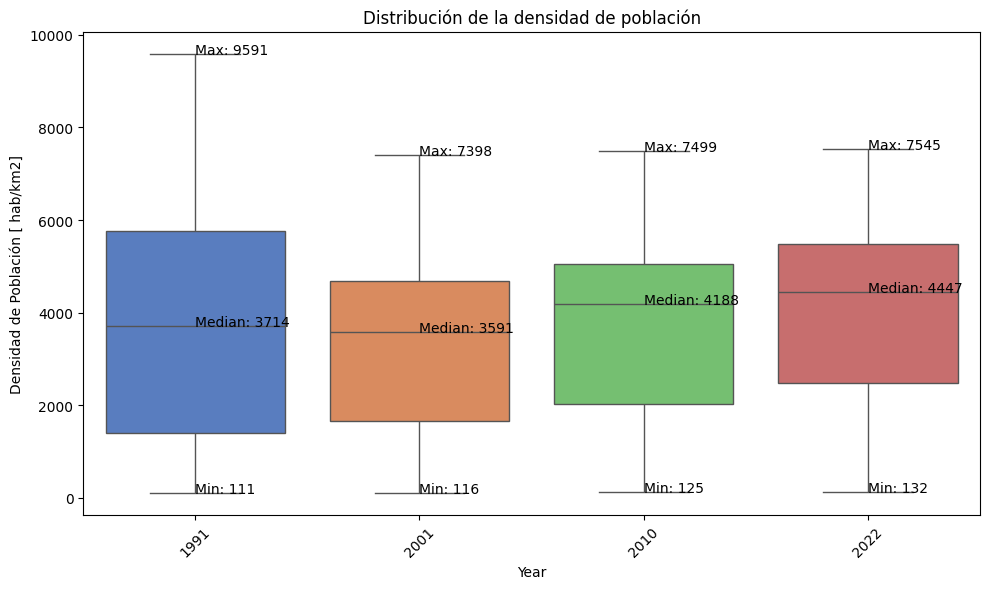
\includegraphics[width=0.45\textwidth]{{C:/Users/Fer/ITBA_TFI/code/latex/img/DensPobBoxplotxAnio.png}}
  \caption{Densidad de Población.Análisis Univariado}
  \label{fig:DensPoblBoxplot}
\end{figure}

\begin{figure}[htbp]
  \centering
  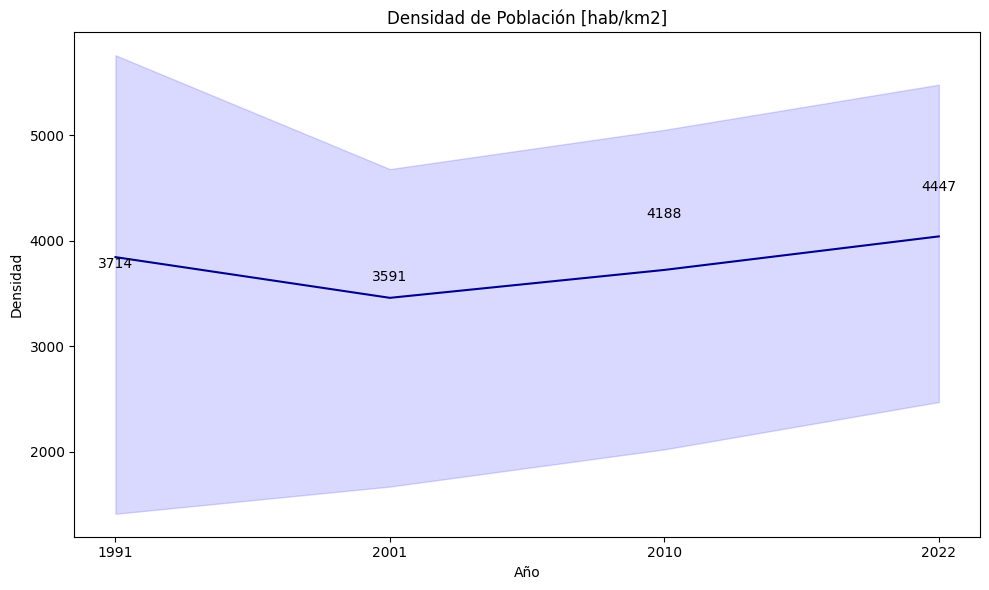
\includegraphics[width=0.45\textwidth]{{C:/Users/Fer/ITBA_TFI/code/latex/img/DensPobTendenciaLinea.png}}
  \caption{Densidad de Población.Análisis Univariado}
  \label{fig:DensPoblLineas}
\end{figure}


\subsubsection{Densidad de Población. Vista geográfica}
Utilizando el sofware QGIS conectado directamente a la base de 
datos AMBA (POSTGRES) se pudo disponer la información de cada Departamento con su geolocalización.
Si bien el distrito más poblado  es La Matanza,bebido su extensión no es el departamento con mayor densidad poblacional en [hab/\textup{km\textsuperscript{2}}] figura \ref{fig:DensidadAll} ,
 los distritos más densamente poblados son Lanús y Vicente López. 


\begin{landscape}
  \begin{figure}[p] % Use 'p' to force the figures to be placed on a separate page
    \centering
    \begin{subfigure}[b]{0.48\textwidth}
        \centering
        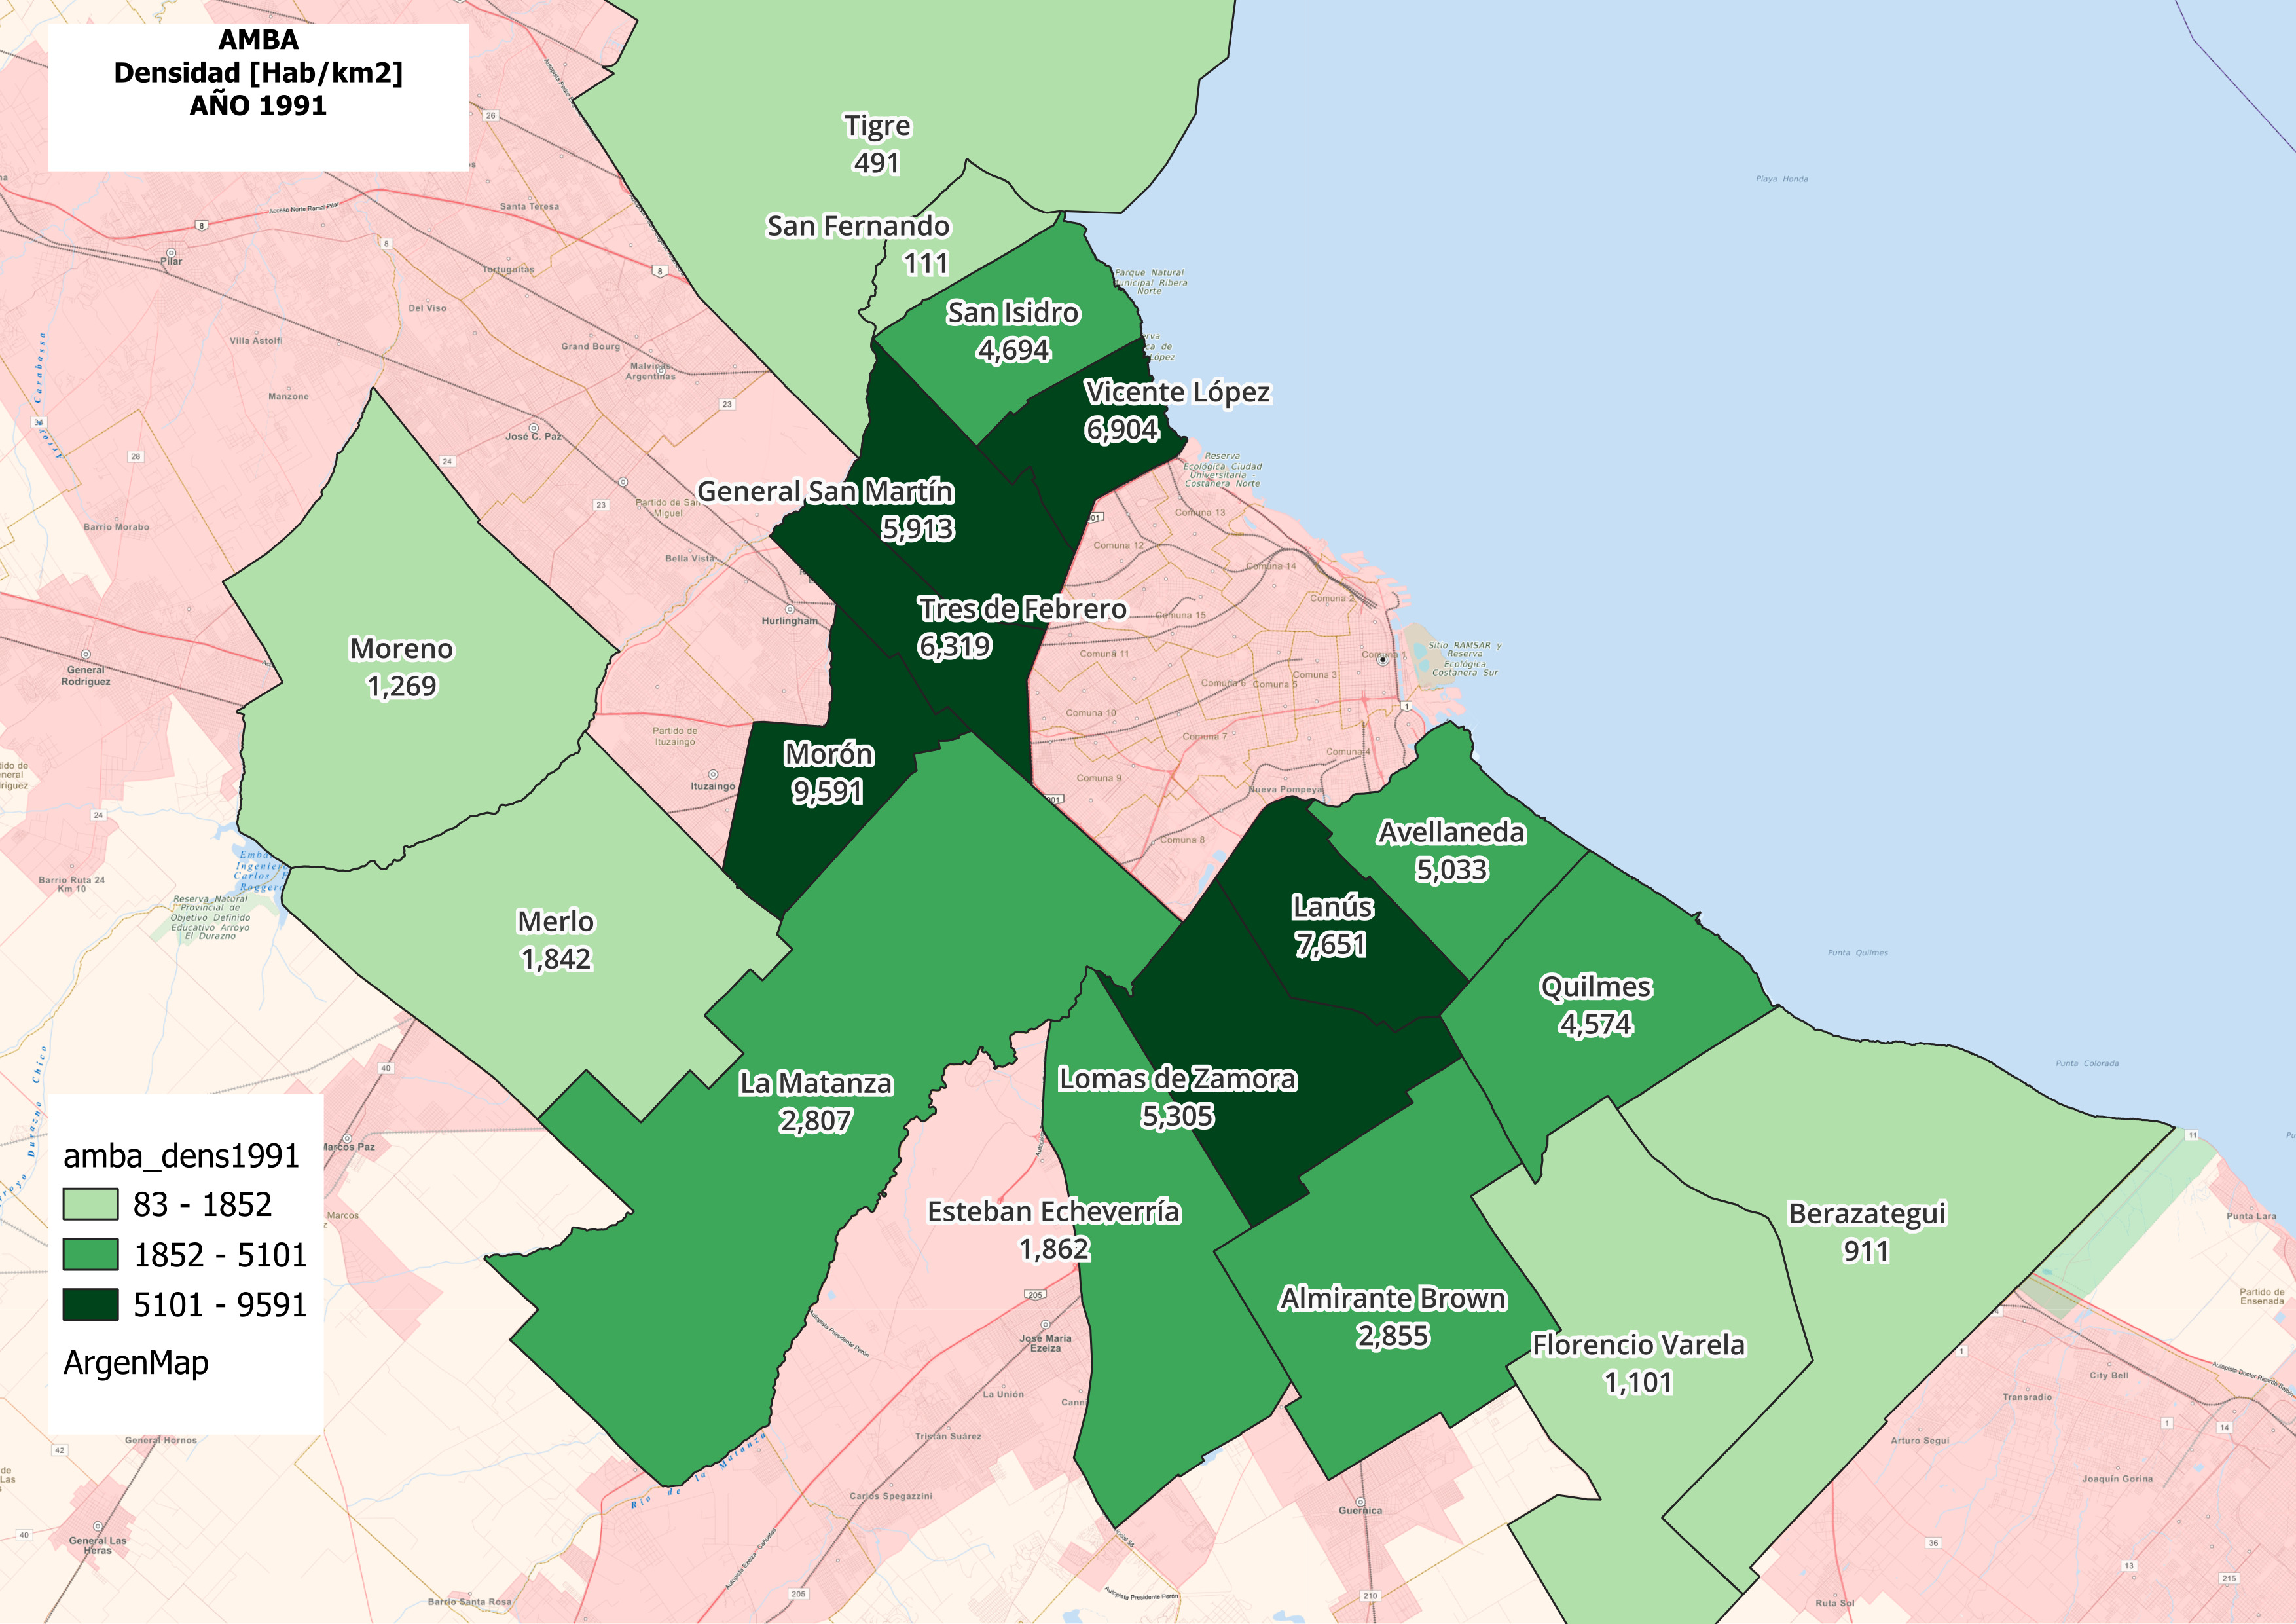
\includegraphics[width=\textwidth]{{C:/Users/Fer/ITBA_TFI/QGIS/img/AmbaDens1991.jpg}}
        \caption{AMBA- Población total Censo 1991}
    \label{fig:dens1991}
    \end{subfigure}
    \quad % Add some horizontal space between subfigures
    \begin{subfigure}[b]{0.48\textwidth}
        \centering
        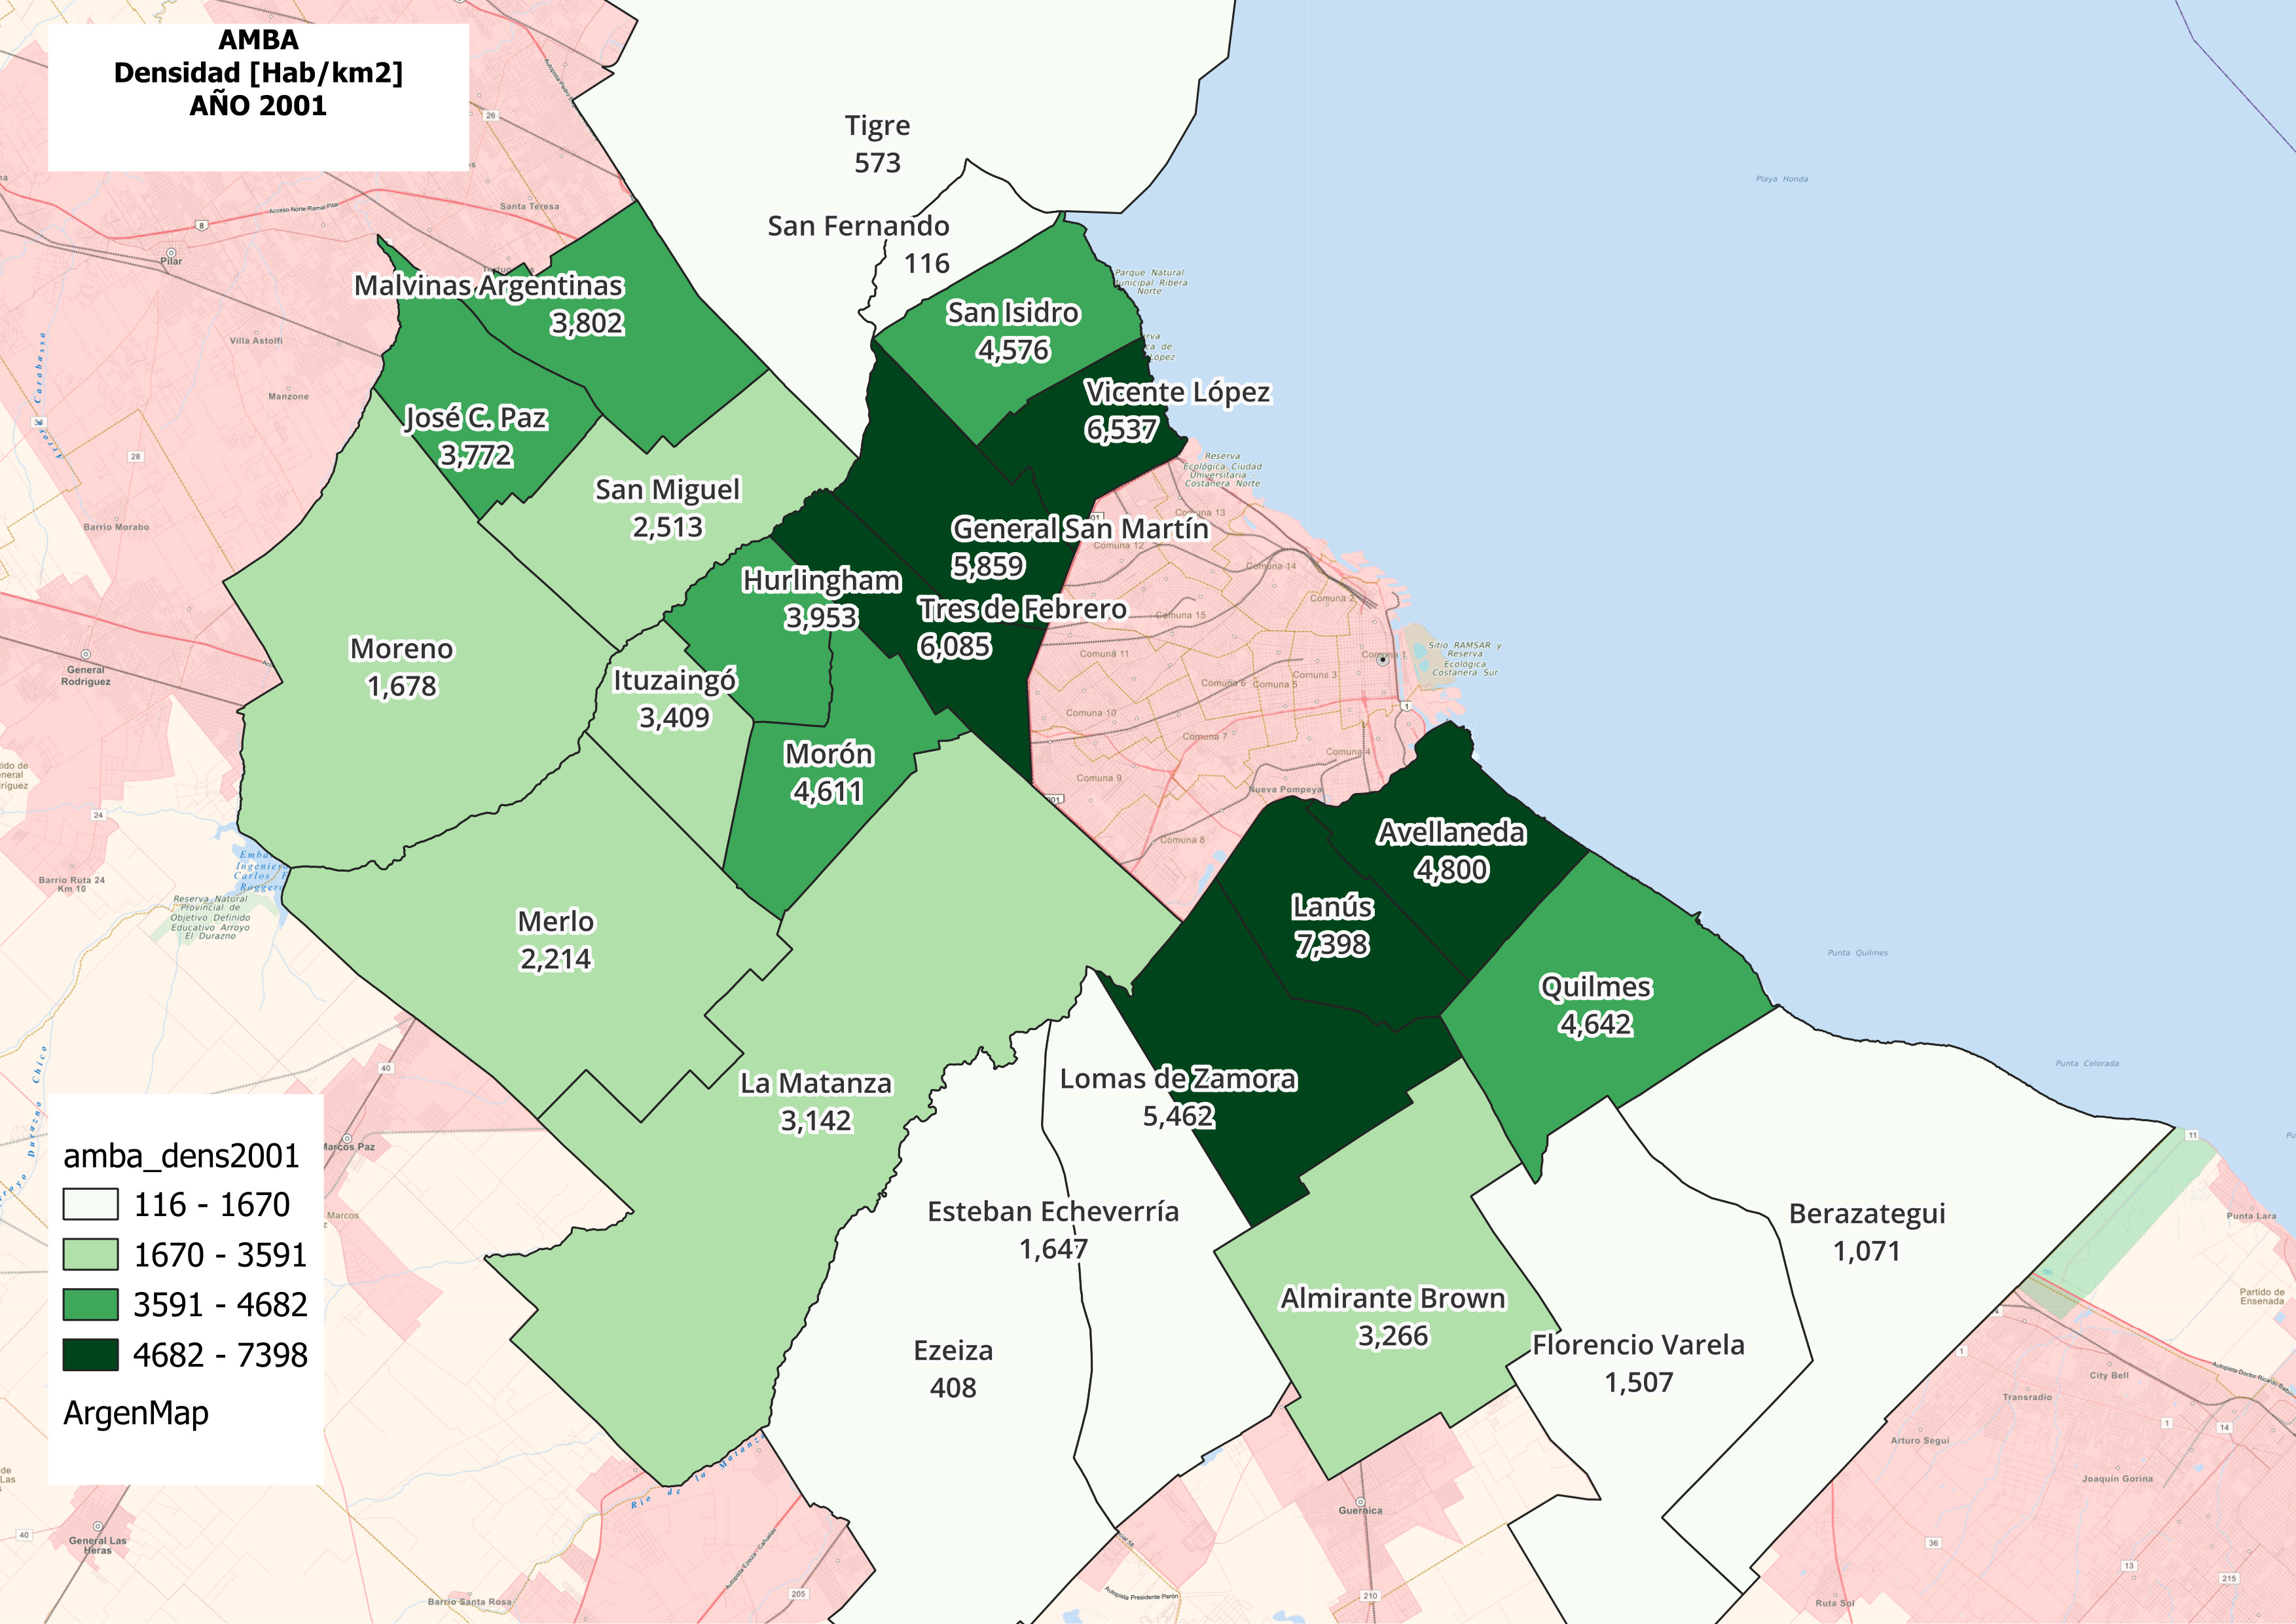
\includegraphics[width=\textwidth]{{C:/Users/Fer/ITBA_TFI/QGIS/img/AmbaDens2001.jpg}}
        \caption{AMBA- Densidad [hab/km2] Censo  2001}
      \label{fig:dens2001}
    \end{subfigure}
    
    \begin{subfigure}[b]{0.48\textwidth}
        \centering
        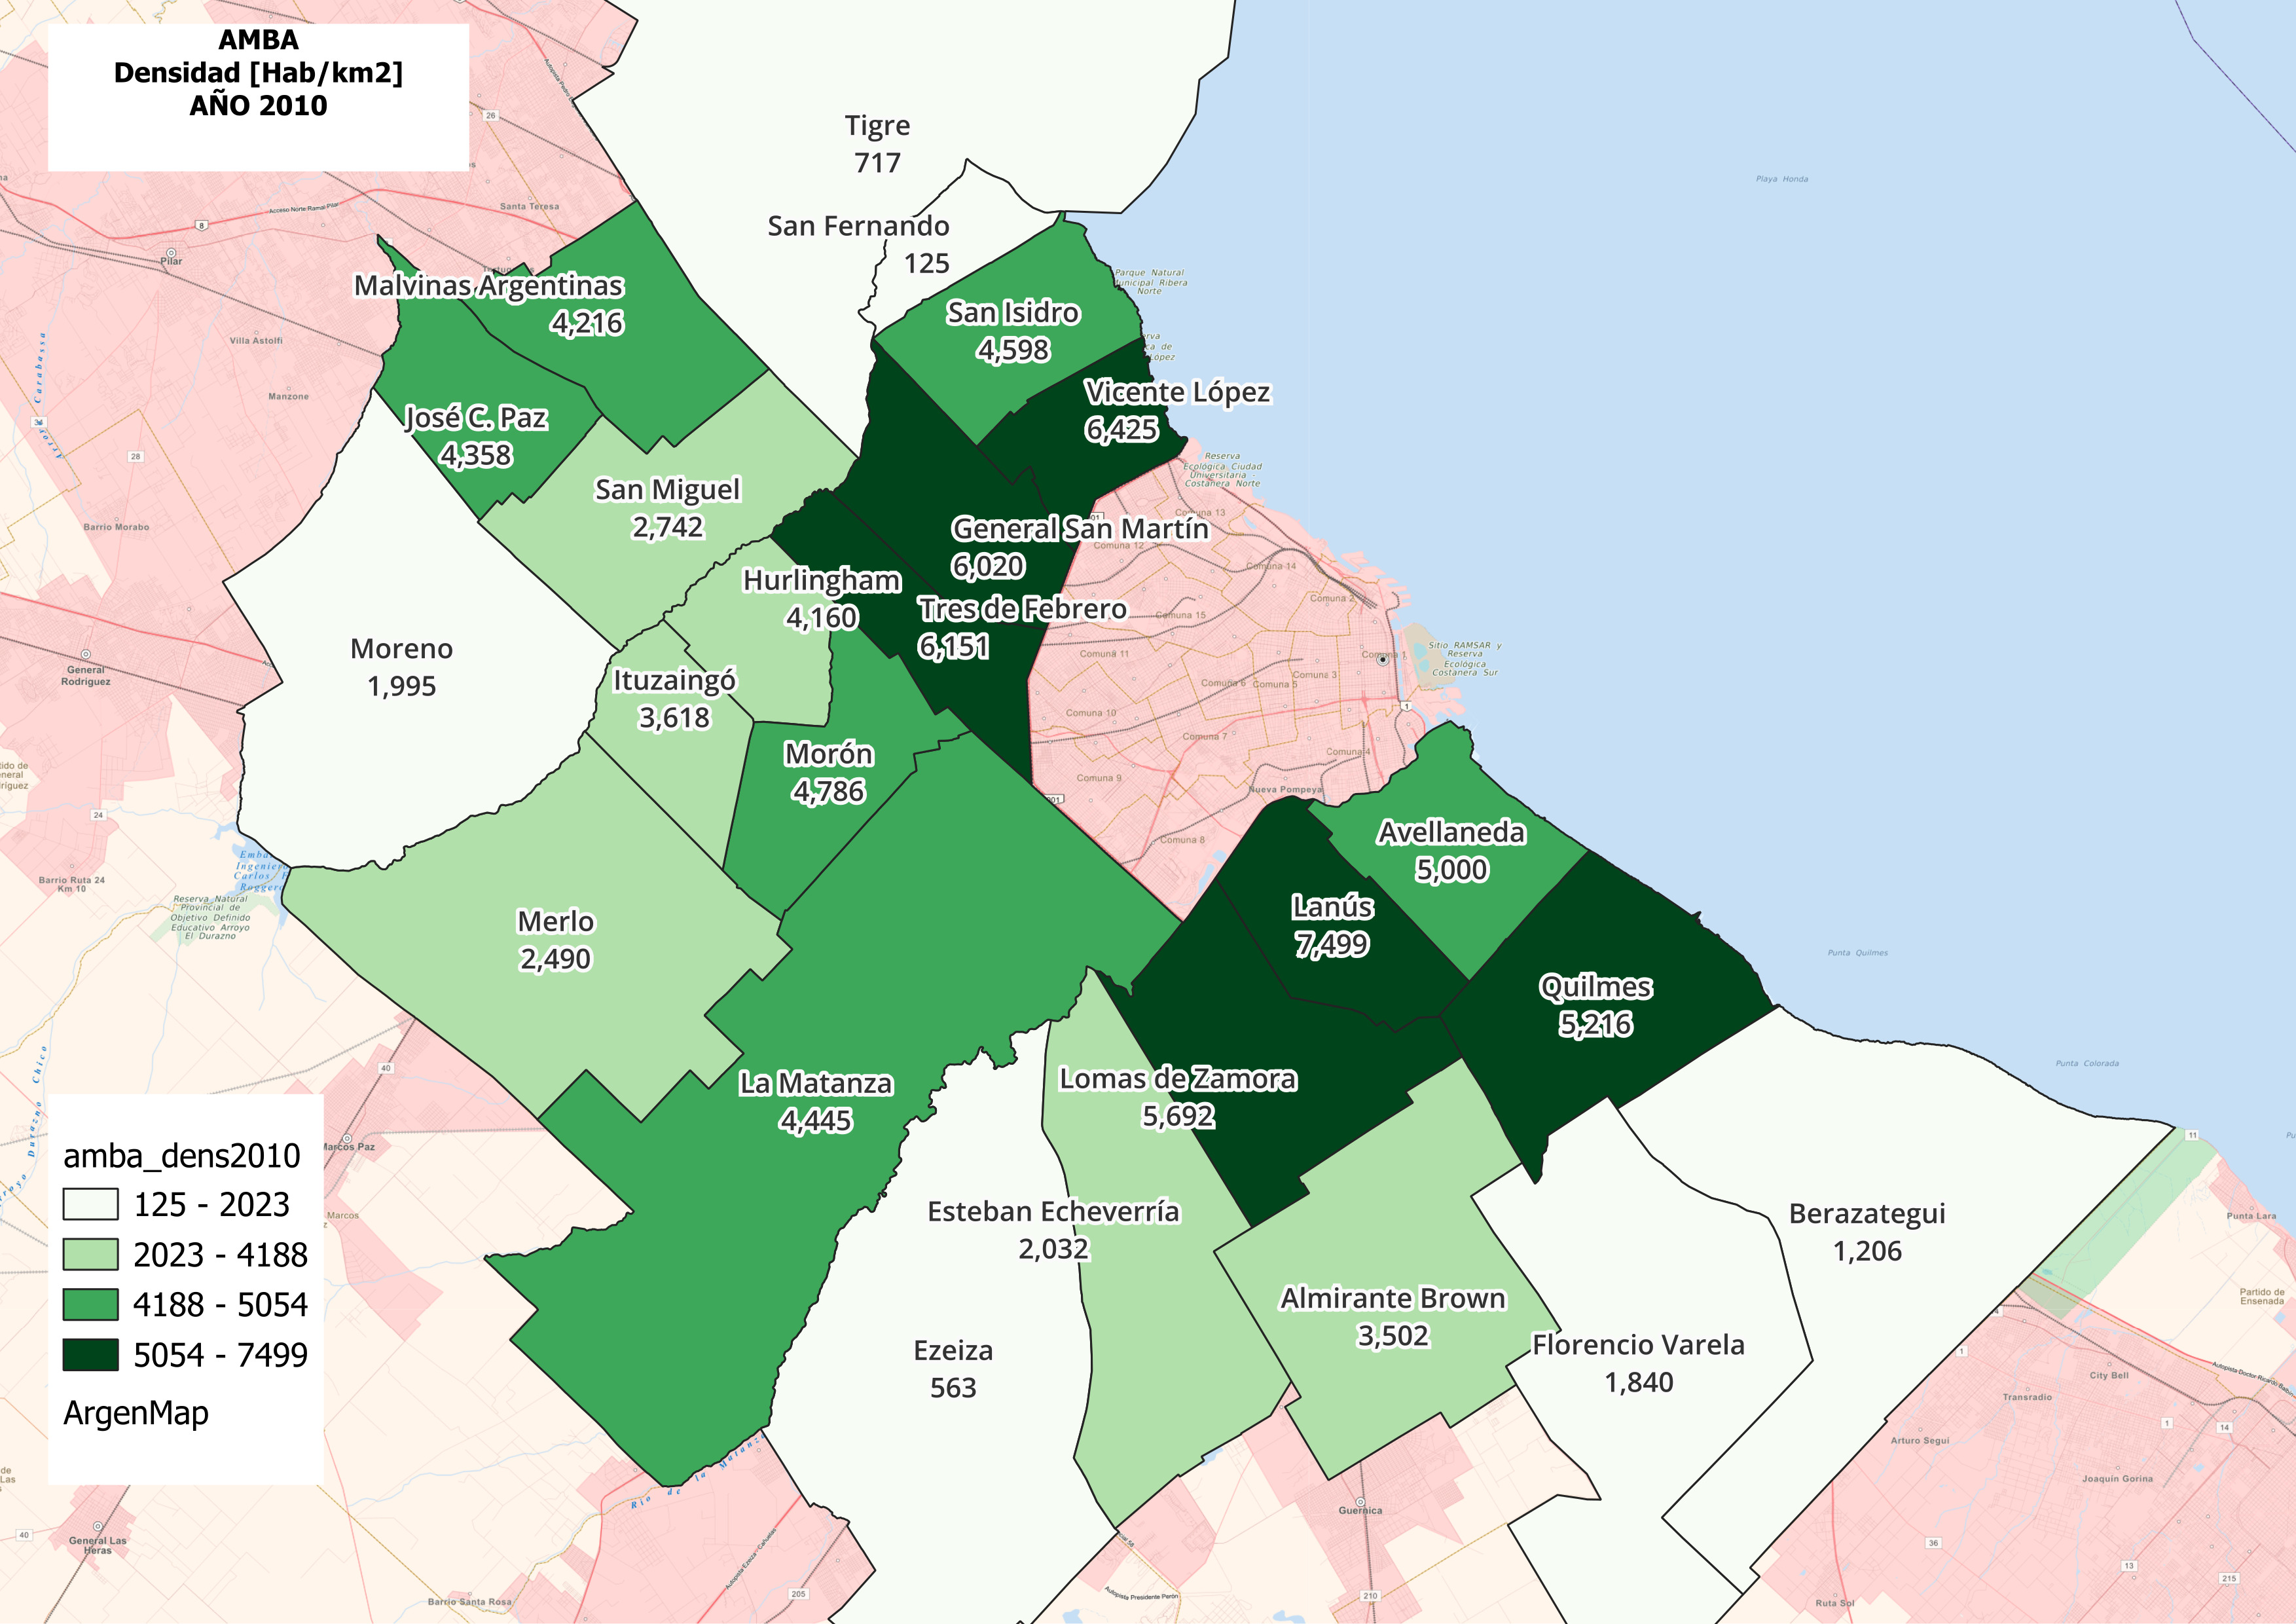
\includegraphics[width=\textwidth]{{C:/Users/Fer/ITBA_TFI/QGIS/img/AmbaDens2010.jpg}}
        \caption{AMBA- Densidad [hab/km2] Censo 2010}
      \label{fig:dens2010}
    \end{subfigure}
    \quad % Add some horizontal space between subfigures
    \begin{subfigure}[b]{0.48\textwidth}
        \centering
        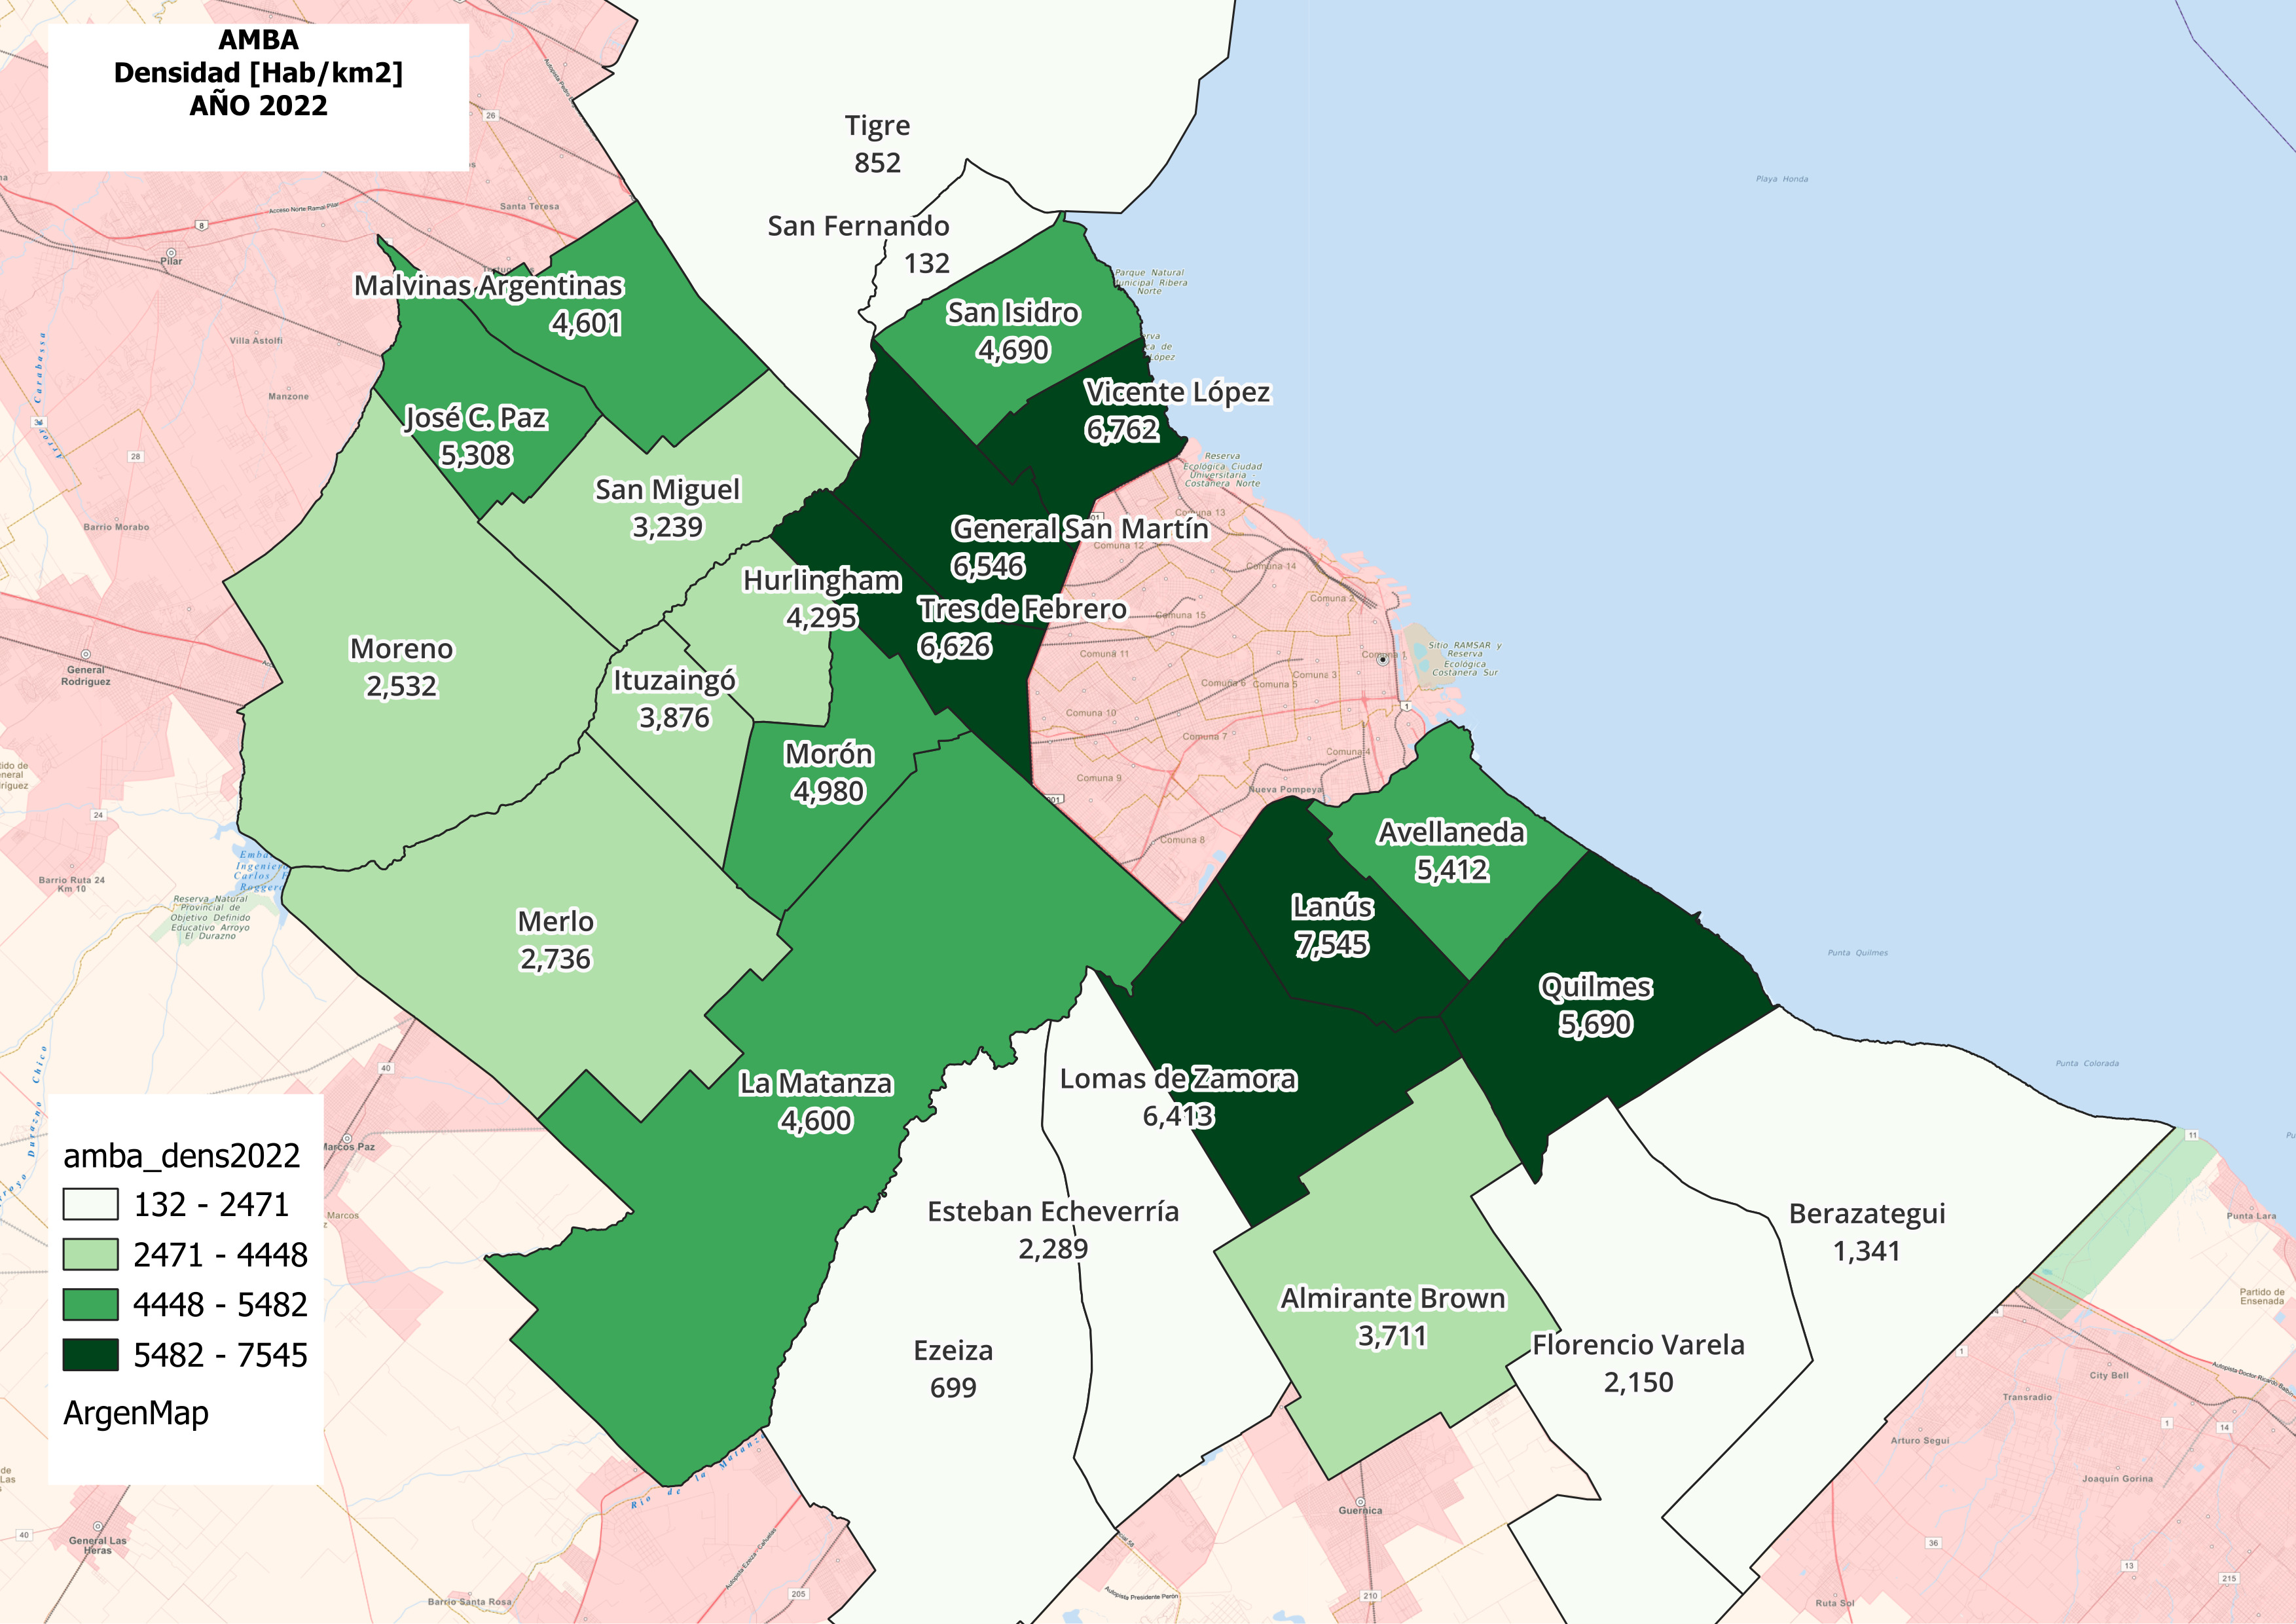
\includegraphics[width=\textwidth]{{C:/Users/Fer/ITBA_TFI/QGIS/img/AmbaDens2022.jpg}}
        \caption{AMBA- Densidad [hab/km2] Censo 2022}
      \label{fig:dens2022}
    \end{subfigure}
    \caption{AMBA- Densidad [hab/km2] Censos 1991 2022}
  \label{fig:DensidadAll}
  \end{figure}
  
  \end{landscape}

\subsection{Tipo de Vivienda}
A partir del censo 2001 se incorpora como atributo descriptivo en cada censo la composición  o tipo de la vivienda, ya sea de tipo particular o colectiva.
Se detalla en cada caso la cantidad de viviendas partciulares('vivpart') en determinado departamento, así como la cantidad de viviendas
colectivas presentes. Se presenta entonces la posibilidad de realizar un analisis univarido del porcentaje de viviendas particulares
respecto al total de viviendas para un determinado departamento y año censal.\newline
Se agrega al dataset una nueva columna definida como:
\begin{equation}
  {\text{VivPart\%}} = 
 \frac{\text{VivPart}}{\text{VivPart} +\text{VivColTot}} \times 100
\end{equation}
Surge de inmediato que mayoría de la población vive en viviendas particulaes (mayor a 99.9\%).Al analizar el comportamiento de este indicador se observa un leve incremento sostenido en el tiempo desde 1991 hasta 2022. 
Es decir que se observan cada vez más peso de las viviendas particulares. El análisis univarido de este indicador puede
observarse en la figura\ref{fig:VivpartBoxplot} así como en la figura\ref{fig:VivpartLines} 
\begin{figure}[htbp]
  \centering
  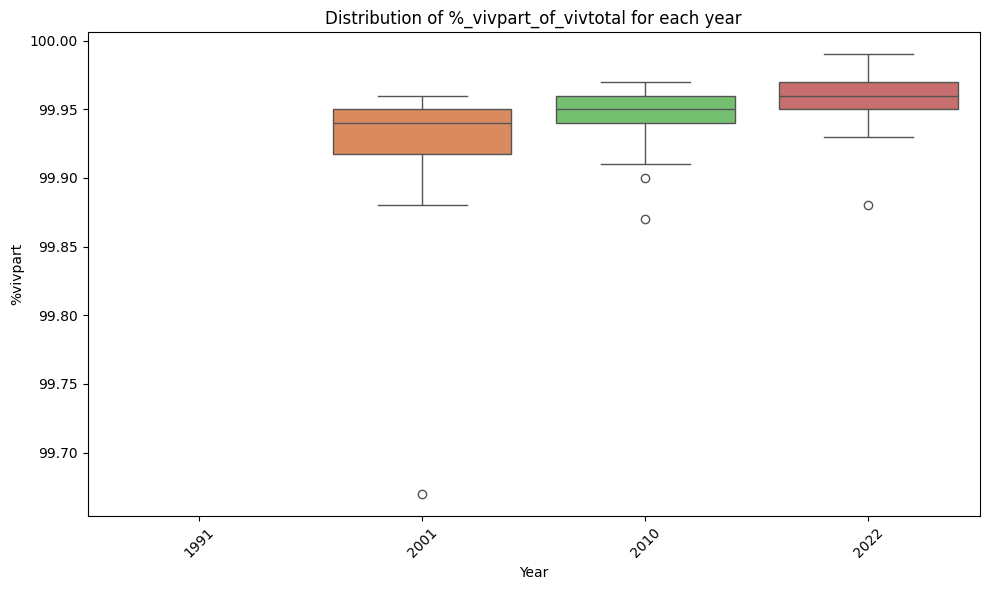
\includegraphics[width=0.45\textwidth]{{C:/Users/Fer/ITBA_TFI/code/latex/img/VivPartxanioBoxplot.png}}
  \caption{Composición de viviendas.Análisis Univariado}
  \label{fig:VivpartBoxplot}
\end{figure}

\begin{figure}[htbp]
  \centering
  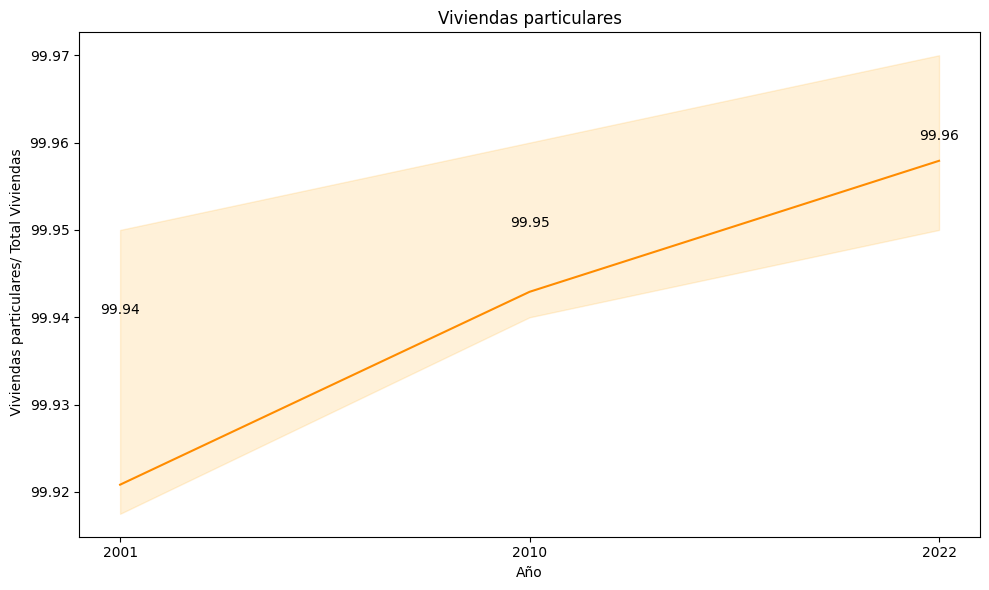
\includegraphics[width=0.45\textwidth]{{C:/Users/Fer/ITBA_TFI/code/latex/img/VivPartTendenciaLinea.png}}
  \caption{Composición de viviendas.Análisis Univariado}
  \label{fig:VivpartLines}
\end{figure}



\subsection{Índice de Masculinidad}
Un indicador habitual de las muestras poblacionales es el índice de masculinidad.
Resultado de dividir el número de hombres entre el número de mujeres de una unidad geográfica o administrativa, 
generalmente multiplicado por 100 expresado como el número de hombres por cada 100 mujeres.
\newline 
Es decir: 
\begin{equation}
  {\text{IndMasc}} = 
 \frac{\text{Varones}}{\text{Mujeres} } \times 100
\end{equation}

Al analizar el comportamiento del ínidice a lo largo del tiempo se observa un descenso sostenido del mismo desde 1991 hasta 2022.
Particularmente el máximo de la muestra presenta un descenso de 5 puntos porcenturales para el año 2022, así como 2 puntos porcentuales la mediana.\newline
 Esto puede observarse en la figura\ref{fig:IndMascBox} así como en la figura\ref{fig:IndMAsvLinea}



\begin{figure}[htbp]
  \centering
  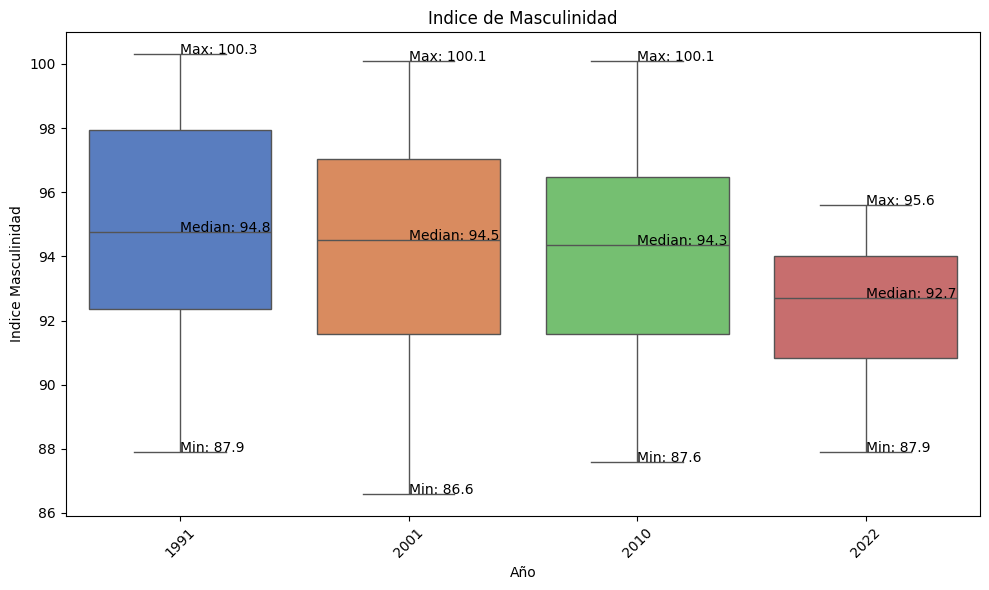
\includegraphics[width=0.45\textwidth]{{C:/Users/Fer/ITBA_TFI/code/latex/img/indMascxAnioBoxplot.png}}
  \caption{Índice de Masculinidad.Análisis Univariado}
\label{fig:IndMascBox}
\end{figure}

\begin{figure}[htbp]
  \centering
  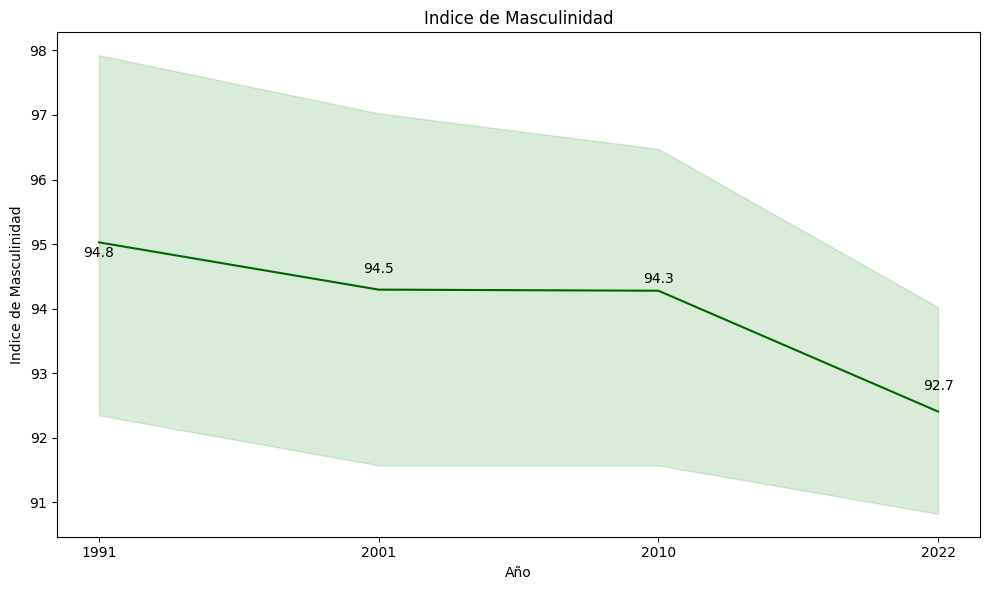
\includegraphics[width=0.45\textwidth]{{C:/Users/Fer/ITBA_TFI/code/latex/img/indMascTendenciaLinea.png}}
  \caption{Índice de Masculinidad.Análisis Univariado}
\label{fig:IndMAsvLinea}
\end{figure}

\section{ Compartiva de los Modelos de Predicción}
 El enfoque en este caso fue el de tomar los censos 1991,2001 y 2010 sumado a las variables sintomáticas antes descriptas
 para  ajustar y entrenar los modelos y luego predecir la población total de cada departmento del AMBA para el Año 2022.
 Al comparar con los resultados publicados por INDEC para el censo 2022 [7**] se determinó la precisión de cada métodología aplicada.\newline 
 Muchas de estas herramientas tiene problemas con los valores nulos o faltantes. Es por esto que los departamentos que no existían en 1991, demandaron 
un tratamiento  especial.
\subsection{Variables Censales}
Respecto a las variables censales podemos decir que presentan una correlación lineal directa muy imporante y
 no aporta variabilidad.Por este motivo no son atributos sginificativos para los modelos propuestos. 
 Para su análisis se utlizó la matriz de correlación, la misma puede verse en la figura\ref{fig:MatCorr} \newline 
 \begin{figure}[htbp]
  \centering
  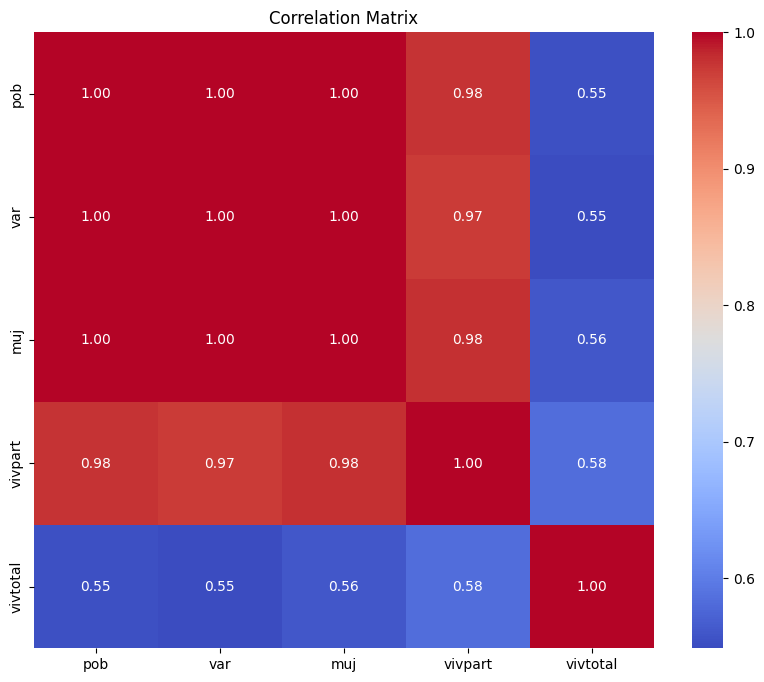
\includegraphics[width=0.8\textwidth]{{C:/Users/Fer/ITBA_TFI/code/latex/img/CorrMatrx.png}}
  \caption{Matriz de correlación . Variables Censales}
  \label{fig:MatCorr}
\end{figure}

\subsection{Errores típicos}
 Para la determinar la precisión y realizar la comparativa entre los modelos aplicados se recurrió a los siguientes errores típicos.\newline
El Error Cuadrático Medio (Mean Squared Error, MSE) es una medida de la calidad de un estimador.
Se calcula promediando el cuadrado de los errores (diferencias entre los valores predichos y los valores reales).\newline

  \[
    \text{MSE} = \frac{1}{n} \sum_{i=1}^{n} (y_i - \hat{y}_i)^2
  \]


 Se calculó también la Raíz del Error Cuadrático Medio (Root Mean Squared Error, RMSE) es la raíz cuadrada del MSE. 
Proporciona una medida de la magnitud promedio del error en las mismas unidades que los valores predichos.\newline   
\[
\text{RMSE} = \sqrt{\frac{1}{n} \sum_{i=1}^{n} (y_i - \hat{y}_i)^2}
\]
 
Asimismo se determinó el Error Porcentual Absoluto Medio (Mean Absolute Percentage Error, MAPE) es 
una medida de precisión que expresa el error como un porcentaje. 
Se calcula promediando el valor absoluto de los errores porcentuales.
\[
\text{MAPE} = \frac{100\%}{n} \sum_{i=1}^{n} \left| \frac{y_i - \hat{y}_i}{y_i} \right|
\]

\subsection{Subset de Datos para Entrenamiento}
 Como se mencionó anteriormente se trabajó con los los censos de los años 1991 , 2001 y 2010. A este conjunto se le agregó el valor
 de las variables sintomáticas para la Jurisdicción provincial- Provincia de Buenos Aires para dichos años.
 Se toma un enfoque planteado por Alvarez en División de Población (2001)\cite{alvarez2001},
entendinedo que el  comportamiento de estas variables puede ayudar a explicar fenómenos a nivel departamental.\newline
 Un esquema del dataset utlizado como input de los modelos puede verse en el cuadro\ref{tab:baseModelos}.


 % Place the table on a landscape page
\afterpage{
  
    \begin{landscape} 
     \begin{table}[htb]
     \centering
      \footnotesize
      \begin{tabular}{|c|c|c|c|c|c|c|c|c|c|c|c|c|c|c|c|c|}
        \hline
        \textbf{\cellcolor[rgb]{0,0.231,0.427}\textcolor{white}{Departamento}} & \textbf{\cellcolor[rgb]{0,0.231,0.427}\textcolor{white}{$cod_depto$}} & \textbf{\cellcolor[rgb]{0,0.231,0.427}\textcolor{white}{ano}} & \textbf{\cellcolor[rgb]{0,0.231,0.427}\textcolor{white}{pob}} & \textbf{\cellcolor[rgb]{0,0.231,0.427}\textcolor{white}{var}} & \textbf{\cellcolor[rgb]{0,0.231,0.427}\textcolor{white}{muj}} & \textbf{\cellcolor[rgb]{0,0.231,0.427}\textcolor{white}{vivpart}} & \textbf{\cellcolor[rgb]{0,0.231,0.427}\textcolor{white}{vivtotal}} & \textbf{\cellcolor[rgb]{0,0.231,0.427}\textcolor{white}{sup}} & \textbf{\cellcolor[rgb]{0,0.231,0.427}\textcolor{white}{$ind_masc$}} & \textbf{\cellcolor[rgb]{0,0.231,0.427}\textcolor{white}{$dens_pob$}} & \textbf{\cellcolor[rgb]{0,0.231,0.427}\textcolor{white}{TMI}} & \textbf{\cellcolor[rgb]{0,0.231,0.427}\textcolor{white}{TGF}} & \textbf{\cellcolor[rgb]{0,0.231,0.427}\textcolor{white}{TBN}} & \textbf{\cellcolor[rgb]{0,0.231,0.427}\textcolor{white}{TBM}} & \textbf{\cellcolor[rgb]{0,0.231,0.427}\textcolor{white}{TCV}} & \textbf{\cellcolor[rgb]{0,0.231,0.427}\textcolor{white}{Mat1ria}} \\ \hline
        Almirante Brown & 6028 & 1991 & 450698.0 & 222042.0 & 228656.0 & nan & nan & 157.87 & 97.1 & 2854.87 & 24.2 & 2.6 & 18.4 & 7.9 & 10.5 & 1752994.0 \\
        Almirante Brown & 6028 & 2001 & 515556.0 & 252454.0 & 263102.0 & 143543.0 & 88.0 & 157.87 & 96.0 & 3265.7 & 15.0 & 2.3 & 16.9 & 8.2 & 8.7 & 1658221.0 \\
        Almirante Brown & 6028 & 2010 & 552902.0 & 270247.0 & 282655.0 & 156218.0 & 78.0 & 157.87 & 95.6 & 3502.26 & 12.0 & 2.5 & 18.9 & 8.4 & 10.5 & 1667278.0 \\
        Avellaneda & 6035 & 1991 & 344991.0 & 164243.0 & 180748.0 & nan & nan & 68.54 & 90.9 & 5033.43 & 24.2 & 2.6 & 18.4 & 7.9 & 10.5 & 1752994.0 \\
        Avellaneda & 6035 & 2001 & 328980.0 & 155450.0 & 173530.0 & 117200.0 & 59.0 & 68.54 & 89.6 & 4799.82 & 15.0 & 2.3 & 16.9 & 8.2 & 8.7 & 1658221.0 \\
        Avellaneda & 6035 & 2010 & 342677.0 & 162264.0 & 180413.0 & 121307.0 & 68.0 & 68.54 & 89.9 & 4999.66 & 12.0 & 2.5 & 18.9 & 8.4 & 10.5 & 1667278.0 \\
        Berazategui & 6091 & 1991 & 244929.0 & 120870.0 & 124059.0 & nan & nan & 268.91 & 97.4 & 910.82 & 24.2 & 2.6 & 18.4 & 7.9 & 10.5 & 1752994.0 \\
        Berazategui & 6091 & 2001 & 287913.0 & 141163.0 & 146750.0 & 81511.0 & 38.0 & 268.91 & 96.2 & 1070.67 & 15.0 & 2.3 & 16.9 & 8.2 & 8.7 & 1658221.0 \\
        Berazategui & 6091 & 2010 & 324244.0 & 158608.0 & 165636.0 & 96029.0 & 37.0 & 268.91 & 95.8 & 1205.77 & 12.0 & 2.5 & 18.9 & 8.4 & 10.5 & 1667278.0 \\
        Esteban Echeverría & 6260 & 1991 & 275793.0 & 136784.0 & 139009.0 & nan & nan & 148.12 & 98.4 & 1861.96 & 24.2 & 2.6 & 18.4 & 7.9 & 10.5 & 1752994.0 \\
        Esteban Echeverría & 6260 & 2001 & 243974.0 & 120110.0 & 123864.0 & 70535.0 & 26.0 & 148.12 & 97.0 & 1647.14 & 15.0 & 2.3 & 16.9 & 8.2 & 8.7 & 1658221.0 \\
        Esteban Echeverría & 6260 & 2010 & 300959.0 & 147980.0 & 152979.0 & 88164.0 & 26.0 & 148.12 & 96.7 & 2031.86 & 12.0 & 2.5 & 18.9 & 8.4 & 10.5 & 1667278.0 \\
        \hline
      \end{tabular}
      \caption{Subset de datos input.Primeras 15 filas. Censos 1991, 2001, 2010 enriquecidos con las variables sintomáticas}
    \label{tab:baseModelos}
    \end{table}
    \end{landscape}
    
 }

 \subsection{Predicciones Población año 2022}
  
 En base al subset de datos predefinido, se entrenoaron los distintos modelos para luego predecir el valor de población total en cada
 departamento para el año 2022. Las predicciones realizadas corresponde a  Regresión Lineal, árbol de decisión (CART), Random Forest , LightGMB
 y también se analizan las estimaciones realizadas por el INDEC en el año 2010. Para cada estimación se obtuvieron los errores 
 típicos. Particularmente para la comparativa de las los modelos se trabaja con el 
 Error Porcentual Absoluto Medio (Mean Absolute Percentage Error, MAPE).\newline

Los resultados obtenidos implican las metodologías tradicionales aproximan mejor este tipo de datos dispersos ''sparse'' poblacionales.Tanto la regresión Lineal ,
como las proyecciones realizadas por el INDEC presentan mejor precisión- menor error- y una menor desviación estándar. Este compartamiento se puede
obsersar en el la figura\ref{fig:BoxPlotModelos}, 
así como el detalle de los estadísticos correspondientes se muestra en el cuadro\ref{tab:EstadModelo}. Las algoritmos de data mining presenta dificultades debido a 
las características particulares de la información censal, el hecho de estar trabajando sólo con la información de 3(tres) Censos Nacionales.Esto sumado al hecho de la granularidad
analizada en este caso, nivel departamental, lo que hace dificil enriquecer el dataset con variables sintomáticas a este nivel y se debe recurrurir a información agregada
a nivel Provincial. Estos modelos presentan valores de error notablemente mayores y una amplia dispesión de resultados.\newline

\begin{figure}[htbp]
  \centering
  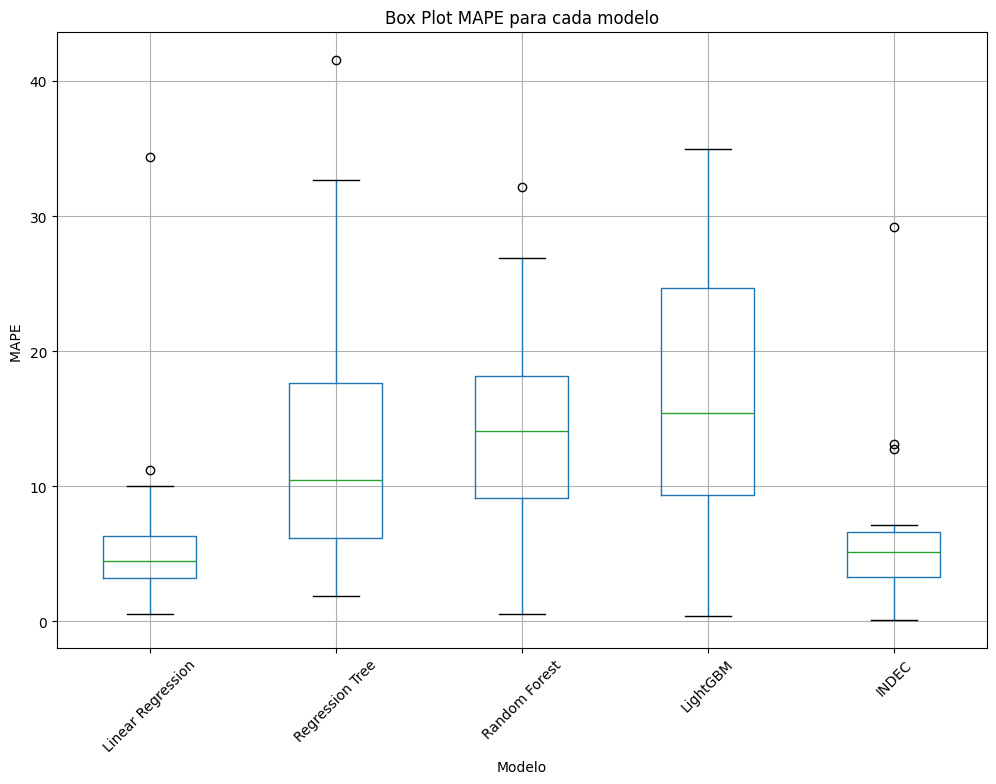
\includegraphics[width=0.8\textwidth]{{C:/Users/Fer/ITBA_TFI/code/latex/img/BoxPlotModels.png}}
  \caption{Box plot del Error Porcentual Absoluto Medio para cada modelo, sobre la predicción población año 2022}
  \label{fig:BoxPlotModelos}
\end{figure}

\begin{table}[htb]
  \centering
  \begin{tabular}{|c|c|c|c|c|c|c|}
  \hline
  \textbf{\cellcolor[rgb]{0,0.231,0.427}\textcolor{white}{Method}} & \textbf{\cellcolor[rgb]{0,0.231,0.427}\textcolor{white}{Q1}} & \textbf{\cellcolor[rgb]{0,0.231,0.427}\textcolor{white}{Median}} & \textbf{\cellcolor[rgb]{0,0.231,0.427}\textcolor{white}{Q3}} & \textbf{\cellcolor[rgb]{0,0.231,0.427}\textcolor{white}{IQR}} & \textbf{\cellcolor[rgb]{0,0.231,0.427}\textcolor{white}{Lower Bound}} & \textbf{\cellcolor[rgb]{0,0.231,0.427}\textcolor{white}{Upper Bound}} \\ \hline
  Linear Regression & 3.2 & 4.5 & 6.3 & 3.1 & -1.4 & 11.0 \\
  Regression Tree & 6.2 & 10.5 & 17.6 & 11.5 & -11.1 & 34.9 \\
  Random Forest & 9.1 & 14.1 & 18.2 & 9.1 & -4.5 & 31.8 \\
  LightGBM & 9.4 & 15.5 & 24.7 & 15.3 & -13.5 & 47.6 \\
  INDEC & 3.3 & 5.1 & 6.6 & 3.3 & -1.6 & 11.6 \\
  \hline
  \end{tabular}
  \caption{Estadísticos MAPE por Modelo}
  \label{tab:EstadModelo}
  \end{table}
  

Los outliers para estos modelos se resumen en el cuadro\ref{tab:DeptOutliers}. Si se analizan los modelos con mejor precisión, en Regresión Lineal tanto
Esteban Echeverría(MAPE:11.2\%) como la Matanza(MAPE:41.6\%) son outliers, donde la predicción estuvo muy alejada del valor
poblacional del CENSO 2022. Para el caso de las proyecciones según INDEC, aparecen también Esteban Echeverría (MAPE:13.1\%) 
y la Matanza (MAPE:29.2\%) como outiliers.  El caso de Esteban Echeverría tiene que ver con la cesión de territorio y cambios administrativos
desde el año 1991 al 2001. Esto implicó que su población descienda entre 1991  y 2001 un -11,5\% mientras que
 entre 2001 y 2010 creció un 23.3\%.
La Matanza presenta entonces singularidades y se comporta distinto de los departamentos aledaños.\newline


\begin{table}[htb]
  \centering
  \begin{tabular}{|c|c|c|c|c|c|}
  \hline
  \textbf{\cellcolor[rgb]{0,0.231,0.427}\textcolor{white}{Departamento}} & \textbf{\cellcolor[rgb]{0,0.231,0.427}\textcolor{white}{$MAPE_LR$}} & \textbf{\cellcolor[rgb]{0,0.231,0.427}\textcolor{white}{$MAPE_RT$}} & \textbf{\cellcolor[rgb]{0,0.231,0.427}\textcolor{white}{$MAPE_RF$}} & \textbf{\cellcolor[rgb]{0,0.231,0.427}\textcolor{white}{$MAPE_LGB$}} & \textbf{\cellcolor[rgb]{0,0.231,0.427}\textcolor{white}{$MAPE_Pred_INDEC$}} \\ \hline
  Esteban Echeverría & \textbf{11.2} & 28.0 & 17.8 & 19.3 & \textbf{13.1} \\
  Ezeiza & 10.0 & \textbf{41.6} &   &   & \textbf{12.8} \\
  La Matanza & \textbf{34.4} & 3.4 & 21.7 & 24.6 & \textbf{29.2} \\
  Moreno & 4.5 & 21.2 & \textbf{32.2} & 35.0 & 2.8 \\
  \hline
  \end{tabular}
  \caption{Outliers por modelo. MAPE .Proyecciones Población 2022}
  \label{tab:DeptOutliers}
\end{table}
  
\subsection{Análisis de Sigularidades. Curva Poblacional La Matanza}

Al analizar la curva poblacional, figura\ref{fig:LMFinalChart} de La Matanza se obervan cambios significativos en el ratio de crecimiento intercensal, a lo largo de los distintos censos.
Si se observa el año 2001 , el ratio intercensal es de 11.9\% que se ubica un 75\% por encima del crecimento(6.8\%) promedio para los municipios del AMBA.
En el año 2010 se observa un ratio de 41.5\% que reprensenta un 250\% por encima del crecimiento promedio( 11.8\%).Esto representa un salto imporante, siendo el municipio que más crecimento
en este periodo. Mientras que para el año 2022 se observa un ratio muy menor del orden de 3.5\% , un 70\% por debajo del crecimiento promedio (10.6\%).\newline
Esto implica que La Matanza es un de los departamento con mayor desviación estandar y coeficiente de variación en
 ratios de creciemiento por departamento,  tal como se describió en apartados anteriores. El creciemiento promedio de los departamentos del AMBA
 para el periodo 1991 a 2010 es de 9,9\% , mientras que La Matanza en el mismo periodo creció un 26,7\% siendo uno de los municipios con mayor crecimiento pobalciona.
 Obviamente el promedio cae al incorporar el año 2022, dando lugar a que La Matanza en toda la serie se acerca al crecimiento promedio de otros municipios.
Seguramente estas sigulardidades hayan dificultado la predicción del valor poblacional para el deparamento con todas la metodologías aplicadas,
 incluyendo aquellas que pudieron resultar mayormente efectivas en la vasta mayoría de los casos.

\begin{figure}[htbp]
  \centering
  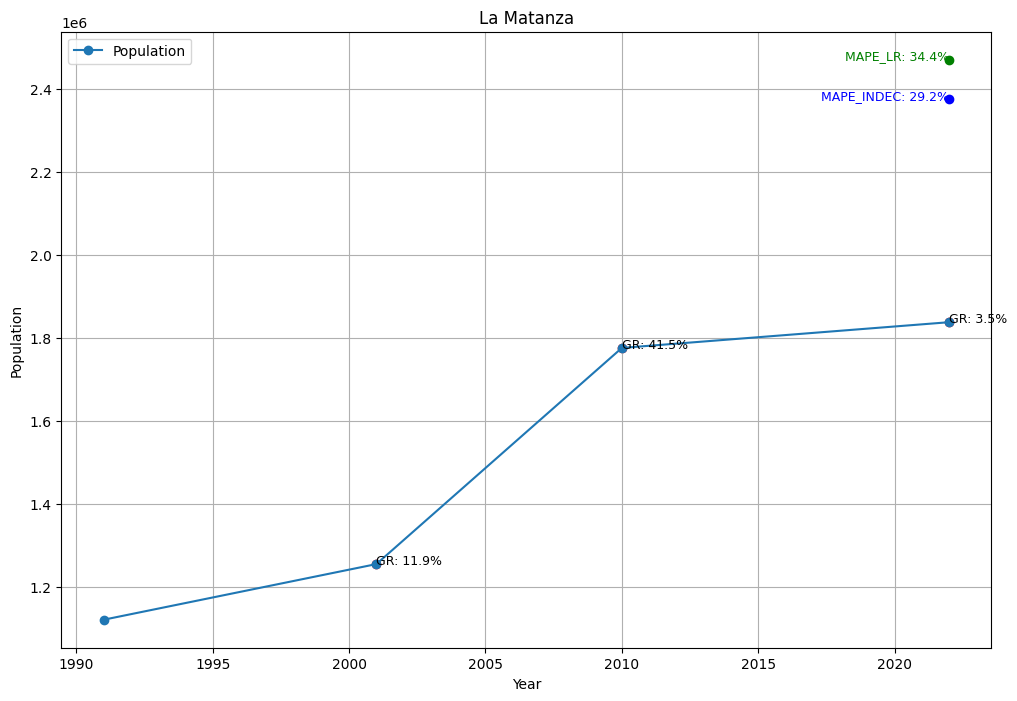
\includegraphics[width=0.8\textwidth]{{C:/Users/Fer/ITBA_TFI/code/latex/img/LMFinalChart.png}}
  \caption{Curva Poblacional La Matanza.}
  \label{fig:LMFinalChart}
\end{figure} 


 \section{Conclusión} 
En resumen, se indica que para la predicción de valores de población a nivel departamentales
 se destacan las metodologías tradicionales, como regresión lineal o bien metodologías que se apoyan en el crecimiento intercensal que comprende la evolución en conjunto
 de las tres variables básicas del análisis demográfico: la fecundidad, la mortalidad y la migración.\newline
  Sin embargo debe
  considerarse que la elaboración de proyecciones de población de áreas menores resulta compleja debido a la imposibilidad de aplicar un método estrictamente demográfico, tal como el método de los componentes, que requiere la estimación y proyección independiente de cada una de las variables del crecimiento
 de la población (fecundidad, mortalidad y migraciones). A este nivel de desagregación, los hechos vitales
 presentan fluctuaciones anuales más acentuadas cuanto menor es el número de población y consecuentemente 
 de nacimientos y defunciones, que pueden afectar las estimaciones de la fecundidad y la mortalidad. Por otra parte estos datos suelen difundirse al público en un nivel de Provicia y no existen datos por Departamento.
 Asimismo, se hace casi imposible la determinación de la migración interna, que suele ser un
 elemento muy importante del crecimiento de dichas áreas. Esto se debe a la dificultad de obtener estimaciones 
 de saldos migratorios consistentes a nivel departamental y a la complejidad para su proyección futura,
 por tratarse de un factor estrechamente asociado a las condiciones económicas y sociales del momento.\newline
Por otro lado puede decirse que las metodologías de data mining no han producido en este caso resultados precisos.
 Prensentan dificultades debido a las características particulares de la información censal,
 el hecho de estar trabajando sólo con la información de 3(tres) Censos Nacionales.Esto sumado al hecho de la granularidad
analizada en este caso, nivel departamental, lo que hace dificil enriquecer el dataset con variables sintomáticas a este nivel y se debe recurrurir a información agregada
a nivel Provincial. Estos modelos presentan valores de error notablemente mayores y una amplia dispesión de resultados.\newline

Ciertamente si bien en la generalidad de los casos es posible estimar un valor población futuro con un grado de confianza aceptable,
 algunos departamentos presentan comportamiento singulares en sus curvas poblacionales que hace imposible su predicción. Las razones de estas singularidades
 escapan al alcance del presente trabajo , bien pueden deberse a causales del  complejo fenómeno demográfico así
  como también errores censales que pudiesen ocurrir.



\section{Referencias bibliográficas}

\begin{enumerate}
  \item  Instituto Nacional de Estadística y Censos \- INDEC.\(2013\). Proyecciones provinciales de población por sexo y grupo de edad 2010-2014. - Instituto Nacional de Estadística y Censos - INDEC, 2013. E-Book. (Vol. 1a ed.).
  %\item Alvarez, G., United Nations. Economic Commission for Latin America and the Caribbean., & CELADE (Organization).
  % División de Población. (2001). Estimación de población en áreas menores mediante variables sintomáticas : una aplicación para los
  % departamentos de la República Argentina (1991 y 1996). Naciones Unidas, CEPAL/ECLAC.
  \item  Instituto Nacional de Estadística y Censos - INDEC. (2015). Estimaciones de población por sexo, departamento y año calendario 2010-2025. (1a. ed.).
  \item Gupta, Arindam , Gupta, Arindam , Gupta, Arindam  (2012).Exploring New Models for Population Prediction in Detecting Demographic Phase Change for Sparse Census Data
  \item  Hoque, Nazrul(2012). Evaluation of small area population estimates produced by Housing Unit, Ratio-correlation, and Component Method II compared to 2000 Census counts. Canadian Studies in Population 39, No. 1–2,  pg. 91-108.
  \item Chawda, Manan, Rane, Rutuja, Giri, Skrinanth(2018) 2nd International Conference on Inventive Communication and Computational Technologies (ICICCT) .Demographic Progress Analysis of Census Data Using Data Mining , pg 1894-1897
  % \item \textbackslash{}.h{INDEC CENSO 2022- $[$Archivo de datos$]$ Recuperado de https://www.censo.gob.ar/index.php/datos_provisionales}
  % \item \textbackslash{https://redatam.org/es}
  % \item \textbackslash{https://redatam.indec.gob.ar/argbin/RpWebEngine.exe/PortalAction?BASE=CPV2010A}
  % \item \textbackslash{https://redatam.indec.gob.ar/argbin/RpWebEngine.exe/PortalAction?BASE=CPV2001ARG}
  % \item  \textbackslash{IGM  Capas SIG - Departamento $[Archivo de datos]$ Recuperado de /https://www.ign.gob.ar/NuestrasActividades/InformacionGeoespacial/CapasSIG}
 %% FUENTES
  \item []Fuente: INDEC. Programa de Análisis Demográfico. Selección de datos tomada de www.indec.gob.ar., Recurso WEB Fecha: 2024-03-29
  %REFERENCIAS ADCICIONALES
  \item []https://data.educacion.gob.ar/reporte-matricula.php
\end{enumerate}


%%%%%%%%%%%%%%%%%%% ANEEEEXOOOOOOOOOOOOOOOOOOOOOOOO%%%%%%%%%%%%%%%%%%%%%%%%%%5

\section{ANEXO}
 \subsection{Diccionario de Departamentos } 
Debido a las inconsistencias y falta de normalización de los archivos CSV que provee el INDEC,
 fue necesaria la creación de un diccionario de departamento asociando las distintas acepciones del nombre de
  departamento con su correspondiente código para que el proceso de ETL pudiese utilizar los códigos de departamento 
  como clave foránea común a todos los Censos Nacionales.
  Se encontraron casos donde el mismo departamento figura nombrado con o sín  tílde,con espacios o abreviaturas en el campo. \newline
De esta forma en la ingesta (ETL) se buscaba el código de departamento correspondiente, que funciona como clave única.
 El formato del diccionario puede verse en el siguiente cuadro\ref{tab:diccionario}.
\begin{table}[htb]
  \centering
  \begin{tabular}{|c|c|}
  \hline
  \textbf{\cellcolor[rgb]{0,0.231,0.427}\textcolor{white}{CodigoDpto}} & \textbf{\cellcolor[rgb]{0,0.231,0.427}\textcolor{white}{Departamento}} \\ \hline
  6005 & General Sarmiento \\
  6005 & General Sarmiento (4) \\
  6260 & Esteban Echeverría (1) \\
  6260 & Esteban Echeverria \\
  6260 & Esteban Echeverría \\
  6270 & Ezeiza \\
  6270 & Ezeiza (2) \\
  6274 & Florencio Varela (3)  \\
  6274 & Florencio Varela \\
  6274 & Florencio Varela (3)  \\
  \hline
  \end{tabular}
  \caption{Diccionario.Primeras 10 filas}
  \label{tab:diccionario}
  \end{table}

 \subsection{Diagrama de entidad relación }
  A modo descrptivo se indica el diagrama de entidad realación de la base de datos confeccionada
  para este trabajo. Figura \ref{fig:DER}.
\begin{figure}[htbp]
    \centering
    \includegraphics[width=0.8\textwidth]{img/DER.jpg}
    \caption{Diagrama de Entidad Relación}
    \label{fig:DER}
\end{figure}

\subsubsection{Script Creación Tablas} 
  \begin{lstlisting}[caption={CreateTables.sql},label={lst:sql_CreateTables}]
    --##POBLACION
        CREATE TABLE IF NOT EXISTS public.poblacion (
        Id SERIAL PRIMARY KEY,
        "AnoCenso" VARCHAR(50),
        "CodigoDpto" VARCHAR(50),
        "Departamento" VARCHAR(150),
        "Poblacion" INT,
        "Varones" INT,
        "Mujeres" INT,
        "VivPartTot" INT,
        "VivColectTot" INT,
        "IndMasc" FLOAT,
      "Superficie" INT,
      "DensPob" FLOAT 
    );
    
    TRUNCATE TABLE public.poblacion;
    
    --## DIM Departamento
    CREATE TABLE IF NOT EXISTS public.DimDepto (
        Id SERIAL PRIMARY KEY,
        "CodigoDpto" VARCHAR(50),
        "Departamento" VARCHAR(150),
        "PartidoFrom" VARCHAR(150),
        "CodigoFrom" VARCHAR(50),
        "Sup1991" INT,
        "Sup2001" INT,
      "IsAMBA" BOOLEAN,
        "Comentarios" VARCHAR(550)
    
    );
    
    TRUNCATE TABLE public.DimDepto;
    
    --##DICCIONARIO DATOS PARTIDO CODIGO
    CREATE TABLE IF NOT EXISTS public.diccionario (
        "CodigoDpto" VARCHAR(50),
        "Departamento" VARCHAR(150)
    );
    
    TRUNCATE TABLE public.diccionario;
    
    --##PROYECCIONES
    CREATE TABLE IF NOT EXISTS public.proyecciones (
        Id SERIAL PRIMARY KEY,
        "CodigoDpto" VARCHAR(50),
        "ano" INT,
        "Departamento" VARCHAR(150),
        "Poblacion" INT,
        "Varones" INT,
        "Mujeres" INT
    );
    
    TRUNCATE TABLE public.proyecciones;
    
    
    ----- GEOMETRY TABLES---
    --1) departamento created from QGIS
    --2) amba+censos
    
    
    ---Now weed need to alter to add  COlumns  para data de los censos
    
    CREATE TABLE  IF NOT EXISTS geo.amba_pob AS
    SELECT *
    FROM geo."vAMBOgeom"
    ALTER TABLE geo.amba_pob 
    ADD COLUMN pob1991 INT,
    ADD COLUMN pob2001 INT,
    ADD COLUMN pob2010 INT,
    ADD COLUMN pob2022 INT;
   ##############
    ALTER TABLE geo.amba_pob 
    ADD COLUMN dens1991 INT,
    ADD COLUMN dens2001 INT,
    ADD COLUMN dens2010 INT,
    ADD COLUMN dens2022 INT;
    
    UPDATE geo.amba_pob AS am
    SET pob1991 = c.pob
    FROM  public.v_censos_amba c
    WHERE am.cod_depto = c.cod_depto AND anio='1991';
    --- Update Poblacion de los censos
    UPDATE geo.amba_pob AS am
    SET pob2001 = c.pob
    FROM  public.v_censos_amba c
    WHERE am.cod_depto = c.cod_depto AND anio='2001';
    
    UPDATE geo.amba_pob AS am
    SET pob2010 = c.pob
    FROM  public.v_censos_amba c
    WHERE am.cod_depto = c.cod_depto AND anio='2010';
    UPDATE geo.amba_pob AS am
    SET pob2022 = c.pob
    FROM  public.v_censos_amba c
    WHERE am.cod_depto = c.cod_depto AND anio='2022';
    
    --- Update DENSIDAD de los censos
    UPDATE geo.amba_pob AS am
    SET dens1991 = c.dens_pob
    FROM  public.v_censos_amba c
    WHERE am.cod_depto = c.cod_depto AND anio='1991';
    UPDATE geo.amba_pob AS am
    SET dens2001 = c.dens_pob
    FROM  public.v_censos_amba c
    WHERE am.cod_depto = c.cod_depto AND anio='2001';
    
    UPDATE geo.amba_pob AS am
    SET dens2010 = c.dens_pob
    FROM  public.v_censos_amba c
    WHERE am.cod_depto = c.cod_depto AND anio='2010';
    UPDATE geo.amba_pob AS am
    SET dens2022 = c.dens_pob
    FROM  public.v_censos_amba c
    WHERE am.cod_depto = c.cod_depto AND anio='2022';
    
  \end{lstlisting}
\subsubsection{Scrip PopulateTables.sql} 
    \begin{lstlisting}[caption={PopulateTables.sql},label={lst:sql_Populate}]
      -- Step 1: Insert data from CSV file without the primary key column
      --- POBLACION START---
      COPY public.poblacion ("AnoCenso", "CodigoDpto", "Departamento", "Poblacion", "Varones", "Mujeres", "VivPartTot", "VivColectTot", "IndMasc","Superficie","DensPob") 
      FROM 'C:/Temp/1991_A~1.CSV' 	
      WITH (FORMAT csv, HEADER true, DELIMITER ';', QUOTE '"', ESCAPE '''', ENCODING 'UTF8');
      
      
      COPY public.poblacion ("AnoCenso", "CodigoDpto", "Departamento", "Poblacion", "Varones", "Mujeres", "VivPartTot", "VivColectTot", "IndMasc","Superficie","DensPob") 
      FROM 'C:/Temp/1991_Resto.CSV' 	
      WITH (FORMAT csv, HEADER true, DELIMITER ';', QUOTE '"', ESCAPE '''', ENCODING 'UTF8');
      
      
      
      COPY public.poblacion ("AnoCenso", "CodigoDpto", "Departamento", "Poblacion", "Varones", "Mujeres", "VivPartTot", "VivColectTot", "IndMasc","Superficie","DensPob") 
      FROM 'C:/Temp/2001.CSV' 	
      WITH (FORMAT csv, HEADER true, DELIMITER ';', QUOTE '"', ESCAPE '''', ENCODING 'UTF8');
      
      
      COPY public.poblacion ("AnoCenso", "CodigoDpto", "Departamento", "Poblacion", "Varones", "Mujeres", "VivPartTot", "VivColectTot", "IndMasc","Superficie","DensPob") 
      FROM 'C:/Temp/2010.CSV'
      WITH (FORMAT csv, HEADER true, DELIMITER ';', QUOTE '"', ESCAPE '''', ENCODING 'UTF8');
      
      
      COPY public.poblacion ("AnoCenso", "CodigoDpto", "Departamento", "Poblacion", "Varones", "Mujeres", "VivPartTot", "VivColectTot", "IndMasc","Superficie","DensPob") 
      FROM 'C:/Temp/2022.CSV'
      WITH (FORMAT csv, HEADER true, DELIMITER ';', QUOTE '"', ESCAPE '''', ENCODING 'UTF8');
      
      -- POBLACION END------
      ---- DICCIONARIO----
      COPY public.diccionario ("CodigoDpto", "Departamento") 
      FROM 'C:/Temp/DiccionarioPartidosCodigo.CSV'
      WITH (FORMAT csv, HEADER true, DELIMITER ';', QUOTE '"', ESCAPE '''', ENCODING 'UTF8');
      
      
      ---	DIMDepto----
      COPY public.dimdepto (
      "CodigoDpto",
      "Departamento",
      "PartidoFrom",
      "CodigoFrom",
      "Sup1991",
      "Sup2001",
      "IsAMBA",
      "Comentarios") 
      FROM 'C:/Temp/DIM Departamento.CSV'
      WITH (FORMAT csv, HEADER true, DELIMITER ';', QUOTE '"', ESCAPE '''', ENCODING 'UTF8');
      
      
      ---	Proyeccion 2025----
      COPY public.proyecciones (
      "CodigoDpto",
      "ano",
      "Departamento",
      "Poblacion",
      "Varones",
      "Mujeres") 
      FROM 'C:/Temp/proy_1025.CSV'
      WITH (FORMAT csv, HEADER true, DELIMITER ';', QUOTE '"', ESCAPE '''', ENCODING 'UTF8');
    \end{lstlisting}


% %% DEFINICIONES
%     La Esperanza de Vida al Nacer es el promedio de años que se espera que viva un recién nacido de 
%     acuerdo con la
%      probabilidad de sobrevivencia prevaleciente en el período del nacimiento.

% %%%%
% La Tasa Bruta de Natalidad es el cociente entre el número de nacimientos ocurridos durante un período determinado, 
% generalmente un año calendario, 
% y la población media del período.
% La Tasa Bruta de Mortalidad es el cociente entre el número de defunciones ocurridas durante un período determinado, 
% generalmente un año calendario, y la población media del período.
% La Tasa de Crecimiento Vegetativo es la diferencia entre entre la Tasa Bruta de Natalidad 
% y la Tasa Bruta de Mortalidad de un período determinado, generalmente un año calendario



%      %%
%      La Tasa Global de Fecundidad es el número de hijos que en promedio tendría una mujer de
%       una cohorte hipotética de mujeres que durante su vida fértil tuvieran sus hijos de acuerdo 
%             a las tasas de fecundidad por edad del período en estudio y no estuvieran expuestas al
%       riesgo de mortalidad desde el nacimiento hasta el término de su período fértil.
% %%%
% La Tasa de Mortalidad Infantil expresa el cociente entre el número de muertes de menores de un año acaecidas 
% en la población de un área geográfica durante un período determinado, 
% generalmente un año calendario, y los nacidos vivos en esa área durante el mismo período.

% %%%
% Índice de envejecimiento de la población: es el cociente entre la población 65 años y más y la población 
% de menores de 15 años de edad.

% %%%
% El porcentaje de población extranjera es el cociente entre la cantidad de 
% habitantes nacidos en el extranjero y el total de la población multiplicado por 100.

\end{document}